\chapter{Groups}
\label{ch:groups}


%\section{Now it starts}
The identity type is not just any type:  in the previous sections we have seen that the identity type $a=_Aa$ reflects the ``symmetries'' of an element $a$ in a type $A$.\footnote{%
  Since the symmetries $p : a=_A a$ are paths that start and end
  at the point $a:A$, we also call them \emph{loops} at $a$.\par
  \begin{tikzpicture}
    \draw plot [smooth cycle] coordinates {(0,0) (2.3,0) (2,1.9) (0,2.1)};
    \node[dot,label=left:$a$] (a) at (0.5,0.3) {};
    \node (A) at (2.5,2.1) {$A$};
    \draw[->] (a) .. controls ++(-10:3) and ++(100:2.5) .. node[auto,swap] {$p$} (a);
  \end{tikzpicture}}
Symmetries have special properties; for instance you can rotate a square by $90\mathdegree$, and you can rotate it by $-90\mathdegree$, undoing the first rotation.
Symmetries can also be composed, and this composition respects certain rules that holds in all examples.  One way to study the concept of ``symmetries'', would be to isolate the common rules for all our examples, but also show, conversely, that anything satisfying these rules actually \emph{is} an example. 



%As an instance of a property that holds in \emph{some} examples but not in others, we have seen that sometimes the order in which we use our symmetries matters, and sometimes it does not, see \cref{ch:intro}.  Hence, the concept of a group should not have a rule allowing you to change the order arbitrarily.

With inspiration of geometric and algebraic origins, it became clear to mathematicians at the end of the 19\textsuperscript{th} century that the properties of such symmetries could be codified by saying that they form an abstract \emph{group}.
In \cref{sec:identity-types} we saw that the identity type was ``reflexive, symmetric and transitive'' -- and an abstract group is just a set with such operations satisfying certain rules.

%This is the purpose of the mathematical term ``group''.

We attack the issue more concretely;
instead of focusing on the abstract properties,
we promote the type exhibiting the symmetries,
and the axioms for an abstract group follow from the rules for identity types
without needing us to worry about them.
However, we \emph{will} show that the two approaches give the same end result.

In this chapter we lay the foundations and provide some basic examples of groups.  

\subsection{Brief overview of the chapter}
In \cref{sec:typegroup} we give the formal definition of a group along with some basic examples.  
In \cref{sec:identity-type-as-abstract} we spell out the details, expanding on the properties of the identity type of a group and comparing these properties with those of an abstract group.  We then return in \cref {sec:identity-type-as-abstract} to groups more generally, explaining how these map to each other through ``homomorphisms'' (which to us are simply pointed maps) and what this entails for the identity types: all the abstract group properties are preserved.  

In most of our exposition we make the blanket assumption that the identity type in question is a set, but in \cref{sec:inftygps} we briefly discuss $\infty$-groups where this assumption is dropped.

Classically, groups have appeared because they ``act'' on a set (or more general objects), that is to say, they collect some of the symmetries of the set.  This is a point of view that we will return to many times and we give the basic theory in \cref{sec:gsets}.  
This section should remind the reader very much of what happened in \cref{cha:circle}, where we did much of the same considerations for the special case of the integers.  
More generally, connected \coverings now reappear in the guise of ``transitive $G$-sets'', laying the groundwork for our later discussion of the set of subgroups.  

Another important thing which is discussed in \cref{sec:gsets} is the type of ``$G$-torsors'', which at first glance can appear frightening.  
However, a $G$-torsor corresponds to \emph{a} universal \covering and the important step is to consider the \emph{type} of these:
This idea is used in \cref{sec:Gsetforabstract} to build the equivalence between our definition of a group and the abstract version taught in most algebra classes.  This is followed up for homomorphisms in \cref{sec:homabsisconcr} and for $G$-sets in \cref{sec:Gsetsabstrconcr}.

With all this in place, the structure of the type of groups is in the large in many aspects similar to the universe in the sense that many of the constructions we're used to from the universe have their analog for groups.
The functions are replaced by the homomorphisms.
Products stay ``the same,'' as we will see in \cref{ex:productofgroups}.
(And more generally, product types over sets ``stay the same.'').
The sum of two groups is simple enough:
It is the sum of the underlying types with the base points identified, as defined more precisely in \cref{def:wedge}.
In the usual treatment this is a somewhat more difficult subject involving ``words'' taken from the two groups.
This reappears in our setting when we show that homomorphisms
from a sum to another group
correspond to pairs of homomorphisms
(just as for sums of types and functions between types).

\footnote{((THEN SUBGROUPS TAKE CENTRAL STAGE, BUT I POSTPONE DISCUSSING THESE IN CASE THIS CHAPTER IS ALREADY OVERLY LONG AND WE WANT TO PUT THEM IN A SEPARATE CHAPTER))}

   


\section{The type of groups}
\label{sec:typegroup}

\begin{definition}
  Given a pointed type $X\jdeq(A,a)$, we define its type of \emph{loops}
  by $\loops X \jdeq (a =_A a)$.
\end{definition}
\begin{example}\label{ex:base=base}
  We defined the circle $\Sc$ in \cref{def:circle} by declaring
  that it has a point $\base$ and an identification (``symmetry'')
  $\Sloop:(\base=\base) \jdeq \loops\Sc$,
  and we proved in \cref{cor:S1groupoid} that $\loops\Sc$ is equivalent
  to the set $\zet$ (of integers),
  where $n\in\zet$ corresponds to the $n$-fold composition of $\Sloop$ with itself
  (which works for both positive and negative $n$).
  We can think of this as describing the symmetries of $\base$:
  we have one ``generating symmetry'' $\Sloop$,
  and this can be applied any number of times,
  giving a new symmetry for each new number.
  Here, composition of loops corresponds to usual addition of integers.

Hence, the circle is a very cheap packaging of the ``{group}'' of integers, the declaration of $\base$ and $\Sloop$ not only gives the \emph{set} $\zet$ of integers, but at the same time the addition.
\end{example}
\begin{example}
  Recall the finite set $\bn{2}:\fin_2$ from \cref{def:finiteset}, containing two elements.   
  According to \cref{xca:C2}, $\bn{2} =\bn{2} $ has exactly two distinct elements,
  $\refl{\bn{2}}$ and $\twist$,
  and doing $\twist$ twice gives you back $\refl{\bn{2}}$.
  We see that this is exactly all the symmetries
  you'd expect to have of a two point set:
  You can let everything stay in place ($\refl{\bn{2}}$),
  or you can swap the two elements ($\twist$);
  and if you swap twice, everything is let be.
  The pointed type $\fin_2$ (of ``finite sets with two elements''),
  with $\bn{2}$ as the base point,
  is our embodiment of these symmetries,\ie $\loops\fin_2$.

  Observe that (by the definition of $\Sc$)
  there is an interesting function $\Sc\to\fin_2$,
  sending $\base:\Sc$ to $\bn{2} :\fin_2$ and $\Sloop$ to $\twist$.
\end{example}

The examples Klein and Lie were interested in were of a type making it admissible to
say that a group is the type of loops $\loops(A,a) \jdeq (a=_Aa)$
for \emph{some} type $A$ and \emph{some} element $a:A$.
However, in elementary texts it is customary to restrict the notion of a group to the case when $a=_Aa$ is a \emph{set}, as we will do, starting in \cref{sec:identity-type-as-abstract}.
This makes some proofs easier, since if are we given two elements $g,h:a=_Aa$, then the identity type $g=h$ is a proposition, \ie $g$ can be equal to $h$ in at most one way.  Hence questions relating to uniqueness will never be a problem.


See \cref{sec:grouphistory} for a brief summary of the early history of groups.
\begin{remark}
  The reader may wonder about the status of the identity type $a=_Aa'$ where $a,a':A$ are different elements.
  One problem is of course that if $p,q:a=_Aa'$,
  there is no obvious way of composing $p$ and $q$
  to get another element in $a=_A a'$,
  and another is that $a=_Aa'$ does not have a distinguished element,
  such as $\refl{a}:a=_Aa$.\footnote{%
    The type $a=_A a'$ does have an interesting \emph{ternary}
    composition, mapping $p,q,r$ to $p\inv{q}r$.
    A set with this kind of operation is called a \emph{heap},
    and we'll return to heaps in \cref{sec:heaps}.}
Given $f:a=_Aa'$ we can use transport along $f$ to compare $a=_Aa'$ with $a=_Aa$ (much as affine planes can be compared with the standard plane or a finite dimensional real vector space is isomorphic to some Euclidean space), but absent the existence and choice of such an $f$ the identity types $a=_Aa'$ and $a=_Aa$ are different animals.  
We will return to this example when we've defined torsors.
\end{remark}


\begin{remark}
  \label{rem:whypointedconngpoid}
% In \cref{xca:component-same-loops} you were asked to show that if $A$ is a type and $a:A$, then 
  As a consequence of \cref{lem:subtype-eq-=},\marginnote{%
    \begin{tikzpicture}
      \draw plot [smooth cycle] coordinates {(0,0) (2.8,0) (2.5,1.9) (0,2.1)};
      \draw[dashed] plot [smooth cycle] coordinates
      {(.1,.1) (1.2,.1) (1,1.5) (.1,1.7)};
      \node[dot,label=left:$a$] (a) at (0.5,.3) {};
      \node[dot,label=right:$b$] (b) at (1.8,.3) {};
      \node (cdots) at (1.8,1.4) {$\cdots$};
      \node (A) at (2.6,2.1) {$A$};
      \node (Aa) at (.7,1.9) {$A_{(a)}$};
      \draw[->] (a) .. controls ++(-10:1) and ++(110:1.6) .. node[auto,swap] {$p$} (a);
      \draw[dashed] plot [smooth cycle] coordinates
      {(1.5,.1) (2.5,.2) (2.6,.8) (1.5,.9)};
      \draw[dashed] plot [smooth cycle] coordinates
      {(1.5,1.1) (2.5,1.2) (2.4,1.8) (1.2,2)};
    \end{tikzpicture}}
  the inclusion of the component $\conncomp A a \defequi \sum_{x:A}\Trunc{a=x}$ into $A$
  (\ie the first projection)
  induces an equivalence of identity types
  from $(a,!)=_{A_{(a)}}(a,!)$ to $a=_Aa$,
  and thus from $\loops(A_{(a)},(a,!))$ to $\loops(A,a)$.
  This means that, when considering the loop type $\loops(A,a)$,
  ``only the elements $x:A$ with $x$ merely equal to $a$ are relevant'',
  and to avoid artificial extra components,
  we should consider only \emph{connected} types $A$ (\cf \cref{def:connected}).

  Also, our preference for $\loops(A,a)$ to be a \emph{set}
  indicates that we should consider only the connected types $A$
  that are \emph{groupoids}.
\end{remark}

\begin{definition}\label{def:pt-conn-groupoid}
  The type of \emph{pointed, connected groupoids} is the type\marginnote{%
    The meaning of the superscript ``${=1}$'' can be explained as follows:
    We also define
    \begin{align*}
      \UU^{\le1}&\defeq\Groupoid\\
      &\defeq
        \sum_{A:\UU}\prod_{x,y:A}\isset(x=_Ay),
    \end{align*}
    to emphasize that groupoids are $1$-types;
    the type of connected types is denoted
    \[
      \UU^{>0} \defeq \sum_{A:\UU}\Bigl(\Trunc{A}\times
    \prod_{x,y:A}\Trunc{x=_ay}\Bigr).\]
    Similar notations with a subscript ``$*$'' indicate pointed types.}
  \[
    \UUscone \defeq \sum_{A:\UU}\sum_{a:A} \Bigl(\isset(a=_Aa)
    \times \prod_{x:A}\Trunc{a=_Ax}\Bigr).
  \]
\end{definition}
The following exercise reconciles the words of the above definition with the type.
\begin{xca}\label{xca:defgroup}
  Show that $A$ is indeed a groupoid for $(A,a,p,q):\UUscone$.
\end{xca}
\begin{remark}
  We shall refer to a pointed connected groupoid $(A,a,p,q)$ simply
  by the pointed type $X \defeq (A,a)$.
  There is no essential ambiguity in this:
  Being a connected groupoid is asserted (for a pointed type) by
  \[
    \isset(a=_Aa)\times\prod_{x:A}\Trunc{a=_Ax},
  \]
  which is a proposition (\cref{lem:prop-utils} and \cref{lem:isX-is-prop}),
  and so the witness $(p,q)$ is unique.

  We also write $\pt_X \defeq a$ for the \emph{base point} of the pointed type.
\end{remark}

We are now ready to define the type of groups:

\begin{definition}\label{def:typegroup}
  The \emph{type of groups} is a wrapped copy (see \cref{sec:unary-sum-types})
  of the type of pointed connected groupoids $\UUscone$,
  \[
    \typegroup \defequi \Copy_{\mkgroup}(\UUscone),
  \]
  with constructor $\mkgroup : \UUscone \to \Group$.
  A \emph{group} is an element of $\typegroup$.
\end{definition}

\begin{definition}\label{def:classifying-type}
  We write $\B : \typegroup \to \UUscone$ for the
  destructor associated with $\Copy_{\mkgroup}(\UUscone)$.
  For $G : \typegroup$,
  we call $\BG$ the \emph{classifying type} of $G$.\footnote{%
    As a notational convention we always write the ``$\B$''
    so that it sits next to and matches the shape
    of its operand.
    You see immediately the typographical reason behind this convention:
    The italic letters $B$,$G$ get along nicely,
    while the roman $\B$ would clash with its italic friend $G$
    if we wrote $\B G$ instead.} % only place \B G is allowed
  Morever, the elements of $\BG$ will be referred to as the \emph{shapes of $G$},
  and we define the \emph{designated shape of $G$} by setting
  $\sh_G\defequi \pt_{\BG}$,
  \ie the designated shape of $G$ is the base point of its
  classifying type.
\end{definition}

\begin{definition}\label{def:group-symmetries}% or elements
  Let $G$ be a group.
  We regard every group as a group of symmetries,
  and thus we refer to the elements of $\loops \BG$ as the
  \emph{symmetries in $G$};
  they are the symmetries of the designated shape $\sh_G$ of $G$.
  (Notice the careful distinction between the phrases
  ``\emph{symmetries in}'' and ``\emph{symmetries of}''.)
  We adopt the notation $\USym G$ for the type $\loops \BG$ of symmetries in $G$;
  it is a set.\footnote{%
    Taking the symmetries in a group
    thus defines a map
    $\USym : \Group \to \Set$,
    with $\mkgroup X \mapsto \loops X$.}
\end{definition}

\begin{remark}\label{rem:aut}
  We are emphasizing that the essential feature of a group
  is the symmetries of its designated shape.
  That is why we defined $\Group$ to be a copy of $\UUscone$,
  and not $\UUscone$ itself;\marginnote{%
    Recall also the example of the negated natural numbers $\NNN$
    from \cref{sec:unary-sum-types}:
    Its elements are $-n$ for $n:\NN$ to remind us how to think about them.
    And the same applies to $\Group$:
    Its elements are $\mkgroup X$ for $X : \UUscone$
    to remind us how to think about them.}
  the type $\USym G$ is at least as important as $\BG$
  --- the copying forces us to use the notation $\BG$,
  preventing a glib identification of $G$ with its classifying type.
  As noted in \cref{sec:unary-sum-types},
  the constructor and destructor pair forms an equivalence $\Group \weq \UUscone$.
  The type $\UUscone$ is a subtype of $\UUp$, so 
  once you know that a pointed type $X$ is a connected groupoid,
  you know also that $X$ is the classifying type for a group,
  namely $G\defeq\mkgroup X$.

  Note that the equivalence also entails
  that identifications $G=H$ of groups are equivalent
  to identifications $\BG = \BH$ of pointed types.
\end{remark}

\begin{remark}\label{rem:BG-convention}
  To define a function $f : \prod_{G:\Group}T(G)$,
  where $T(G)$ is a type family indexed by $G:\Group$,
  it suffices to consider the case $G\jdeq\mkgroup X$,
  where $X$ is a pointed connected groupoid,
  namely the classifying type $\BG$.\footnote{%
    If you are bothered by the convention
    to write the classifying type of $G$ in \emph{italic} like a variable,
    you can either think of $\BG$ as a locally defined
    variable denoting the classifying type that is
    defined whenever a variable $G$ of type $\Group$ is introduced,
    or you can imagine that whenever such a $G$ is introduced
    (with the goal of making a construction or proving a proposition),
    we silently apply the induction principle to
    reveal a wrapped variable $\BG:\UUscone$.}
\end{remark}

It is not infrequent that we want to consider the symmetries $\loops(A,a)$
of some element $a$ in some groupoid $A$.
\begin{definition}\label{def:automorphism-group}
  % Previously, this allowed for A to not necessarily be a groupoid,
  % as long as the component of A is. That seems like unnecessary generality?!
  For a groupoid $A$ with a specified point $a$,
  we define the \emph{automorphism group} of $a:A$ by
  \[
    \Aut_A(a) \defeq \mkgroup (A_{(a)},(a,!)),
  \]
  \ie $\Aut_A(a)$ is the group with classifying type
  $\BAut_A(a) \jdeq (A_{(a)},(a,!))$,
  the connected component of $A$ containing $a$, pointed at $a$.
\end{definition}
\begin{remark}
  \label{rem:symmetriesofnonconnectedgroupoids}
  For any $G \jdeq \mkgroup(A,a) : \Group$, we have an identification
  $G = \Aut_A(a)$,
  because we have an identification of pointed types $(A_{(a)},(a,!)) = (A,a)$,
  since $A$ is connected.

  In other words, for any $G \jdeq \mkgroup\BG$, we have
  an identification $G = \Aut_{\BG}(\sh_G)$, of $G$ with the automorphism
  group of the designated shape $\sh_G : \BG$.
\end{remark}

\subsection{First examples}
\label{sec:firstgroupexamples}
   \begin{example}\label{excirclegroup}
   The circle $S^1$, which we defined in \cref{def:circle}, is a connected groupoid (\cref{lem:circleisconnected}, \cref{cor:S1groupoid}) and is pointed at $\base$. The identity type $\base=_{S^1}\base$ is equivalent to to the set of integers $\zet$ and composition corresponds to addition.  This justifies our definition of the \emph{group of integers} as 
$$\ZZ \defeq \aut_{S^1}(\base).$$
It is noteworthy that along the way we gave several versions of the circle, each of which has its own merits, the version in \cref{def:S1toC}
$$C=(\sum_{X:\UU}\sum_{f:X=X}\Trunc{(\zet,s)=(X,f)}, (\zet,s))$$
being a very convenient one.
 \end{example}

\begin{example}\label{ex:groups}
  % Since any pointed connected groupoid is a group, there is no shortage of examples, but perhaps i
  Apart from the circle, there are some important groups that come almost for free: namely the symmetries in the type of sets.
%It is worthwhile to consider some specially designed examples.
  \begin{enumerate}
  \item Recall that the set $\bn{1} =\true$ has the single element which we can call $*$. Then $\aut_{\bn{1} }(*)$ is a group called the \emph{trivial group}.
  \item If $n:\NN$, then the \emph{permutation group of $n$ letters} is 
$$\Sigma_n\defequi\aut_{\fin_n}(\bn{n} ),$$ 
where $\fin_n$ is the groupoid of sets of cardinality $n$ (\cf \ref{def:finiteset}).  
The classifying type is thus $B\Sigma_n\defequi (\fin_n,\bn{n})$.
With our convention of \cref{rem:symmetriesofnonconnectedgroupoids} we can tolerate $\aut_{\fin}(\bn n)$, $\aut_{\Set}(\bn n)$ or even $\aut_{\UU}(\bn n)$ as synonyms for the group $\Sigma_n$ (where $\fin$ and $\Set$ are the subtypes of $\UU$ of finite sets and sets).  

If the reader starts worrying about size issues, that is quite legitimate; see \cref{rem:groupsarebig}.
% DELETE Note that even though the sets $\bn{n} =_{\fin}\bn{n} $ and $\bn{n} =_{\fin_n}\bn{n} $ are equal, we must use the component $\fin_n$ rather than the entire groupoid $\fin$ of finite sets to keep the underlying pointed groupoid $B\Sigma_n=(\fin_n,\bn{n} )$ connected.
  \item More generally, if $S$ is a set, is there a pointed connected groupoid $(A,a)$ so that $a=_Aa$ models all the ``permutations'' $S=_{\Set}S$ of $S$?  Again, the only thing wrong with the groupoid $\Set$ of set (apart from $\Set$ being large) is that $\Set$ is not connected. 
%}!\footnote{it's so simple -- so very simple -- that only a child can do it!}  To be precise, the component of $S$ is
%$$A\defequi\sum_{X\in\Set}\Trunc{S=X}.$$  
%The connected groupoid $\sum_{X\in\Set}\Trunc{S=X}$ is pointed at $S$ (and the fact that $S=S$ is nonempty since $\refl S:S=S$).    
% Then 
% $$(S=_AS)=(S=_{\Set}S)$$ 
% (in the identity type of a $\Sigma$-type both the first and the second projections must be equal, but for $A\oldequiv\sum_{X:\Set}\Trunc{S=X}$ the second projection is a proposition).  
%
 The \emph{group of permutations of $S$} is defined to be 
$$\Sigma_{S}\defequi\aut_{\Set}(S),$$  
with classifying type $B\Sigma_S\defequi(\conncomp \Set S,S)$.
% DELETE SINCE WERE NOT TALKING ABT INFTYGPS Likewise, if $X$ is any type, the \emph{group of automorphism} or \emph{permutations} of $X$ is defined to be 
% $$\Sigma_X=\aut_{\UU_{(X)}}X,$$
%  where $U_{(X)}$ is the component of $\UU$ containing $X$.
  \end{enumerate}
\end{example}

\begin{remark}
  \label{rem:groupsarebig}
  This is only for those who worry about size issues - a theme we systematically ignore in our exposition.  If we start with a base universe $\UU_0$, the groupoid of sets of cardinality $n$, $\fin_n$ is a $\Sigma$-type $\sum_{A:\UU_0}\Trunc{A=\bn{n}}$ over $\UU_0$ and so without any massage will lie in a bigger universe $\UU_1$.  In order to accommodate for the finite permutation groups, the universe ``$\UU$'' appearing as a subscript for the first $\Sigma$ in the definition of groups needs to be at least as big as $\UU_1$.  If so, the type $\typegroup$ will not be in $\UU_1$, but in some bigger universe $\UU_2$, so if I choose some group $G$ and look at \emph{its} group of automorphisms, this will will be a group only if the universe is at least as big as $\UU_2$.  Luckily, our convention is that the universes are nested, and so at any point we'll just be somewhere big enough for our purposes, see \cref{sec:univax}.  This is not to say that these questions are trivial or unimportant; they are nontrivial and important, but not what this text is about.
\end{remark}

\begin{example}\label{ex:cyclicgroups}
In \cref{thm:coveringsofS1} we studied the symmetries of the ``$m$-fold \covering'' 
of the circle for $m$ a positive integer, and showed that there were $m$ different
such symmetries. Moreover we showed that these symmetries were the powers $f^n$ (for $n=0,1,\dots,m-1$)
of one (non-unique) symmetry $f$ and that $f^{m+k}=f^k$ for any integer $k$.
This very important phenomenon pops up in many situations, 
and is called the \emph{cyclic group of order $m$}.
In other words, the cyclic group of order $m$ is the (pointed) component of the type $\SetBundle(\Sc)$ of \coverings of the circle containing the $m$-fold \covering.
We analyzed this in \cref{thm:coveringsofS1} and found that this (pointed) component was equivalent to the connected groupoid
$$B\ZZ/m_\div\defequi\conncomp{(\sum_{X:\Set}X=X)}{\zet/m}$$
pointed in $\zet/m = (\bn{m},s_n),$
where 
$$s_n :\bn{m}=\bn{m}$$ is (the identity corresponding to the equivalence given by) 
the cyclic permutation of $\bn{m}$, sending $m-1$ to $0$ and, 
for $0\leq i<m-1$, sending $i:\bn m$ to $i+1$ (strictly speaking, $\zet/m$ when first presented in Definition~\ref{def:Zetmodm} represented a symmetry of $\bn m\times\bn 1$, but we trust we'll be forgiven for retaining the names of the symmetry under identification provided by univalence and the projection from $\bn m\times \bn1$ to $\bn m$). The role
the successor function plays in $C$ is played by the successor modulo $m$ in $\ZZ/m$. 

It is this modular behavior which inspires the ``$\ZZ/m$'' in the expression above: we are talking about the ``integers modulo $m$''.
We make this our (first) definition of the cyclic group of order $m$:
\end{example}
\begin{definition}\label{def:Z/mgroup}
  If $m$ is a positive integer, the cyclic group of order $m$ is the group
  $$\ZZ/m\defequi\aut_{B\ZZ/m}(\zet/m).$$
\end{definition}


\begin{example}

There are other (beside the symmetries of the $m$-fold \covering and Definition~\ref{def:Z/mgroup}) ways of obtaining the cyclic group of order $m$, which occasionally are more convenient.  The prime other interpretation is as the group of ``cyclic permutations of $m$ points on a circle''; \ie as the ``set of $m$th roots of unity in the complex plane'' equipped with complex multiplication.  

We know the group $\Sigma_m\defequi\aut_{\fin_m}(\bn m)$ of {\bf all} permutations of the set $\bn m$ with $m$ elements, but how do we select the ``subgroup'' of cyclic permutations?  
The key insight is the provided by function 
$$cy_m:S^1\to\fin_m$$ 
with $cy_m(\base)\defequi\bn m$ and 
$cy_m(\Sloop)\defis s_m$, picking out exactly the cyclic permutation $s_m\colon\bn m=\bn m$ (and its iterates) among all permutations.  Set truncation of \cref{def:set-truncation} provides us with a tool for capturing only the symmetries of $\fin_m$ hit by $f$: the (in language to come) subgroup of the permutation group of cyclic permutations is the group
$$C_m\defequi\aut_{BC_m}(\pt_{C_m}),$$
where $(BC_m)_\div\defequi \sum_{S:\fin_m}\Trunc{cy_m^{-1}(S)}_0$ and $\pt_{C_m}\defequi (\bn m,\trunc{(\base,\refl{\bn m})}_0))$.  We must prove that $BC_m$ is a pointed connected groupoid for it to earn the name ``group'', but since we will provide a pointed equivalence between $B\ZZ/m$ and $BC_m$, this will follow automatically.

More precisely, but using language not yet established, this is shown in ???\footnote{find reference} as applied to the map $cy_m\colon S^1\to\fin_m$ (interpreted as a ``group homomorphism'' $cy_m\colon \ZZ\to\Sigma_n$): $\ZZ/m$ is equivalent to the ``quotient group'' (\cf \cref{def:normalquotient}) of $\ZZ$ by the ``kernel'' (\cf \cref{def:kernel}) of $cy_m$, whereas $C_m$ is exactly the ``image'' (\cf \cref{def:image}) of $cy_m$.  

However, in our special case we can give a proof using only language we know.
Consider $t:\prod_{z:S^1}((\base=\base)\to(z=z))$ given by circle induction by sending $\base:S^1$ to the identity $t_\base\defequi\id_{\base=\base}$ and $\Sloop:\base=\base$ to $\refl{\id_{\base=\base}}$.
Since we'll be using it often, we let $\Sloop_z:z=z$ be shorthand for $t_z(\Sloop)$.
\footnote{is this how you would like to say it: it should be conjugation, but perhaps you argue for this through commutativity?} 

\begin{lemma}
  Given $S\colon\fin_m$, the function 
  \begin{align*}
    f_S\colon\Sigma_{z\colon\Sc^1}(S=cy_m(z))&\to \Sigma_{q\colon S=S}\Trunc{(S,q)=(\bn m,s_m)},\\
 f_S(z,v)&\defequi (v^{-1}cy_m(\Sloop_z)v,!)
  \end{align*}
  has connected fiber and defines 
 an equivalence $f\colon BC_m\we B\ZZ/m$.
\end{lemma}
\begin{proof}
  First and foremost, $f_S$ is actually well defined in the sense that $(S,v^{-1}cy_m(\Sloop_z)v)=(\bn m,s_m)$ is inhabited.
  This is clear in view of the function
  $$(\base =z)\to((S,q)=(\bn m,s_m))$$
  sending $p:\base= z$ to the identity represented by the picture
  $$\xymatrix{
    \bn m\ar@{=}[ddd]^{s_m}\ar@{=}[r]^-{\refl{} }& cy_m(\base)\ar@{=}[ddd]^{cy_m(\Sloop)}\ar@{=}[r]^{cy_m(p)}&cy_m(z)\ar@{=}[ddd]^{cy_m(\Sloop_z)}\ar@{=}[r]^-v&S\ar@{=}[d]^-v\\
    &&&cy_m(z)\ar@{=}[d]^{cy_m(\Sloop_z)}\\
     &&&cy_m(z)\ar@{=}[d]^-v\\
     \bn m\ar@{=}[r]^-{\refl{} }& cy_m(\base)\ar@{=}[r]^{cy_m(p)}&cy_m(z)\ar@{=}[r]^-v&\,S,}
  $$
  where leftmost square commutes by definition of $cy_m$, the center square commutes by the definition as $\Sloop_z$ by circle induction and the rightmost square commutes by associativity.

  Note that  once we have shown that $f_S$ has connected fiber, we know that the set truncation $\Trunc{f_S}_0$ is an equivalence;
  % and in view of the commutativity of 
  $$\xymatrix{\Sigma_{z\colon\Sc^1}(S=cy_m(z))\ar[r]^-{f_S}\ar[d]& \Sigma_{q\colon S=S}\Trunc{(S,q)=(\bn m,s_m)}\ar[d]^{\simeq}\\
 \Trunc{\Sigma_{z\colon\Sc^1}(S=cy_m(z))}_0\ar[r]^-{\Trunc{f_S}_0}& \Trunc{\Sigma_{q\colon S=S}\Trunc{(S,q)=(\bn m,s_m)}}_0 }
  $$ and the fact that $\Sigma_{q\colon S=S}\Trunc{(S,q)=(\bn m,s_m)}$ is a set gives us (upon applying $\Sigma_{S:\fin_m}$) the desired equivalence $BC_m\we B\ZZ_m$.

  So to finish the proof we must show that $f_S$ has connected fiber.
  Since $S$ lies in the component of $\bn m\oldequiv cy_m(\base)$ and since the proposition $\Trunc{(cy_m(\base),q)=(\bn m,s_m)}$ implies that $q$ is identical to $\Sloop^k$ for some $k$, it suffices to prove that for every $k$ the fiber
  $f_{cy_m(\base)}^{-1}(cy_m(\Sloop^k),!)$ -- or written out:
  $$\Sigma_{z:S^1}\Sigma_{v:\bn cy_m(\base)=cy_m z}cy_m(\Sloop^k)=v^{-1}cy_m(\Sloop_z)v$$
   -- is connected.

  Assume $(z,v,!):f_{cy_m(\base)}^{-1}(\Sloop^k,!)$.  Given $p:\base=z$ we get that the diagram
  $$\xymatrix{cy_m(\base)\ar@{=}[r]^{cy_m(p)}\ar@{=}[d]^{cy_m(\Sloop}&cy_m(z)\ar@{=}[r]^-v&cy_m(\base)\ar@{=}[d]^{cy_m(\Sloop}\\
  cy_m(\base)\ar@{=}[r]^{cy_m(p)}&cy_m(z)\ar@{=}[r]^-v&cy_m(\base)}$$
commutes; that is, $cy_m(p)v:cy_m(\base)=cy_m(\base)$ commutes with $cy_m(\Sloop)$.
Consequently, $cy_m(p)v$ must be of the form $cy_m(\Sloop^k)$ for some $k=0,1,\dots,m-1$, or alternatively, we have an $\alpha:v=cy_m(p^{-1}\Sloop^k)$.
Hence $(p^{-1}\Sloop^k,\alpha):(z,v,!)=(\base,\refl{})$.

{\color{red}This was not the most elegant thing I've produced, but I must quit now and push so that you can see if you get the gist.  I'll put arrows on the =s when I get around to it}
\end{proof}


% THE REST IS TO BE DELETED WHEN THE ABOVE IS FINISHED.

% Staying close to the type $C$ above is perhaps the simplest: %\cref{def:S1toC}
% $$BC_m\defequi(\sum_{X:\Set}\sum_{p:X=X}\Trunc{(\bn{n},s_m)=(X,p)},(\bn{n},s_m)),$$


% For yet another way of obtaining $C_m$, consider the function 
% $$cy_m:S^1\to\fin_m$$ 
% with $cy_m(\base)\defequi\bn n$ and 
% $cy_m(\Sloop)\defis s_m$.  
% Note that the symmetry $cy_m(\Sloop)$ is cyclic in the sense that 
% the $n$-fold iterate $cy_m(\Sloop)^n$ is $\refl{\bn n}$.
% Then the $n$-fold \covering can be seen as the first projection 
% $$\sum_{z:S^1}cy_m(z)\to S^1$$
% (you are asked to write this out in \cref{xca:somedetailsonfinitegroupstocheck}).
% Consider the pointed type 
% \[
% B_m\defequi(\sum_{S:\fin_m}\Trunc{cy_m^{-1}(S)}_0 ~,~ 
% (\bn n,\trunc{(\base,\refl{\bn n})}_0))
% \]
% where the type can be viewed as the ``image'' of $cy_m$,
% except that the truncation is one level higher than we have considered before.
% Since $\fin_m$ is a groupoid, $B_m$ is a groupoid. 
  
% If we focus on the point $\pt_{B_m}\defequi(\bn n,\trunc{(\base,\refl{\bn n})}_0)$ and 
% write out the identity type $\pt_{B_m}=\pt_{B_m}$ of the $\Sigma$-type $B_m$, 
% we see that it consists of those $p:\bn n=\bn n$ such that there is 
% a $q:\base=\base$ with $p=cy_m(q)$: 
% the ``permutations that come from rotating $n$ points on the circle'' -- 
% exactly what the cyclic group of order $n$ should be!

% We DOUBLY define {\em cyclic group of order $n$} to be the group (DELETE?)
% $$C_m\defequi\aut_{B_m}(\pt_{B_m}).$$

% It is good to know that $B_m$ is connected, so that $(B_m,\pt_{B_m})$ is actually 
% AAAthe classifying type [DELETE $BC_m$. NOT YET PROVED: ISOMORPHIC ABSTRACT
%  GROUPS HAVE EQUIVALENT CLASSIFYING TYPES] Remember that 
% $cy_m^{-1}(S)\defequi\sum_{z:S^1}(S=cy_m(z))$, and notice that the map 
% $$e:\sum_{S:\fin_m}cy_m^{-1}(S)\to S^1,\qquad e(S,z,p)=z$$ 
% is an equivalence fitting in a commuting diagram [CHECK LOOP?]
% $$\xymatrix{
% \sum_{S:\fin_m}cy_m^{-1}(S)\ar[d]^e_\simeq\ar[rr]^-{\text{set truncation}}&&
% \sum_{S:\fin_m}\Trunc{cy_m^{-1}(S)}_0\ar[d]^{\text{first projection}}&\oldequiv B_m\\
% S^1\ar[rr]^{cy_m}&&\,\fin_m.}$$
% All preimages of of the top map are all inhabited, and since $S^1$ is connected, 
% the source is connected.  
% Hence \cref{lem:whenisbasespaceconnected} tells us that $B_m$ is connected too.


% % .  Let $(S,z,p):B_m$ be any element; we want to show that $(S,z,p)=_{B_m}(\bn n, \base, \refl\base)$ is not empty, so that $B_m$ is connected. Since $S^1$ is connected there is a $q:z=_{S^1}\base$ so $(cy_m(q)\,p,q,!):(S,z,p)=(\bn n,\base,\refl\base)$ (using that $cy_m(\base)\defequi\bn n$ to compose $p:S=cy_m(z)$ and $cy_m:cy_m(z)=cy_m\base$), $B_m$ is connected.  
% % DELETE Pointing $B_m$ in $\pt_{C_m}$ we have a pointed connected groupoid, \ie a group, which we call the {\em cyclic group $C_m$ of order $n$}  (and in hindsight $B_m=(BC_m)_\div$).

Note that the cyclic group of order $1$ is the trivial group, the cyclic group of order $2$ is equivalent to the permutation group $\Sigma_2$: there are exactly one nontrivial symmetry $f$ and $f^2$ is the identity.  When $m>2$ the cyclic group of order $m$ is a group that does not appear elsewhere in our current list.  In particular, the cyclic group of order $m$ has only $m$ different symmetries, whereas we will see that the group of permutations $\Sigma_m$ has $m!=1\cdot 2\cdot\dots\cdot m$ symmetries.
\end{example}

\begin{example}\label{ex:productofgroups}
  If you have two groups $G$ and $H$, their \emph{product} $G\times H$ is given by taking the product of their classifying types:
  \[
    G\times H\defequi \mkgroup(\BG\times\BH)
  \]
  (Note that $\B(G\times H)\jdeq \BG\times \BH$ is pointed at
  $\sh_{G\times H}\jdeq(\sh_G,\sh_H)$.)
  For instance, $\Sigma_2\times\Sigma_2$ is called the
  \emph{Klein group}.\footnote{%
    Also known as the \emph{Vierergruppe} or
    the \emph{Klein four-group}, because
    it has four symmetries.}
\end{example}

\footnote{We might tone down exercises like ``prove that $\typegroup$ is a groupoid'', even though we will want to use these results.  They take the geometry/fun out of the exposition.}
\begin{xca}
  \label{xca:somedetailsonfinitegroupstocheck}
  \begin{enumerate}
  \item Compare the definitions of \cref{def:finiteset} and show that if $n:\NN$, then $\Sigma_n=\Sigma_{\bn{n} }$ %is equal to the permutation group on $n$ letters 
and (since $\fin_0=\fin_1=\bn 1$) that $\Sigma_{1}=\aut_{\bn{1} }(\triv)$.
%\item Display an element in $\bn{2} =_{\fin_2}\bn{2} $ different from $\refl{\bn{2} }$ in the group $\Sigma_{2}$ of permutations of two letters.  
\item Prove that the set $\bn{n} =_{\fin_n}\bn{n} $ is finite of cardinality $n!$.
\item Give an identification of the $n$-fold \covering of $S^1$ of \cref{exa:mfoldS1cover} with the first projection $\sum_{z:S^1}cy_n^{-1}(z)\to S^1$ of \cref{ex:cyclicgroups}.
%, where $cy_n:S^1\to\fin_n$ is given by $cy_n(\base)\defequi\bn n$ and $cy_n(\Sloop):\bn n=\bn n$ is cyclic permutation (sending $n-1$ to $0$ and, for $0\leq i<n-1$, sending $i:\bn n$ to $i+1$).  

Hint: for every $z:S^1$, $cy_n(z):\fin_n$ is a finite set of cardinality $n$.  
Decidability is not an issue, so you can appeal to our classification of the \coverings of the circle.
\item Show that, given a type $X$, the type of functions $BC_n\to X$ is equivalent to the type 
$$\sum_{f:S^1\to X}\prod_{z:S^1}f(z)=f(z^n)$$ of functions $f:S^1\to X$ such that the two ways around
$$\xymatrix{S^1\ar[d]_{(-)^n}\ar[dr]^f&\\S^1\ar[r]^f&X}$$
agree. Hint: define the function $F_1:(BC_n\to X)\to (S^1\to X)$ by precomposition:
$F_1(g)(z)=g(cy_n(z),!)$ and observe that since $cy_n(z)=cy_n(z^n)$ we have a 
function $F:(BC_n\to X)\to \sum_{f:S^1\to X}\prod_{z:S^1}f(z)=f(z^n)$.
\end{enumerate} 
\end{xca}

\begin{remark}
In \cref{lem:idtypesgiveabstractgroups} we will see that the identity type of a group satisfies a list of laws justifying the name ``group''
%we may associate an abstract group $(a=_Aa,e,{-}^{-1},\cdot)$
and we will later show that groups are uniquely characterized by these laws.
\end{remark}
Some groups have the property that the order you perform the symmetries is immaterial.  The prime example is the group of integers $\ZZ\oldequiv \aut_{S^1}(\base)$  Any symmetry is of the form $\Sloop^n$ for some integer $n$, and if $\Sloop^m$, then $\Sloop^n\Sloop^m=\Sloop^{n+m}=\Sloop^{m+n}=\Sloop^m\Sloop^n$.

 Such cases are important enough to have their own name:
\begin{definition}\label{def:abgp}
  A group $G$ is \emph{abelian} if %all symmetries commute in the sense that 
the proposition
$$\mathbf{isAb}(G)\defequi\prod_{g,h: \USym G}gh=hg$$
is true.  In other words, the type of abelian groups is 
$$\mathbf{Ab}\defequi \sum_{G:\typegroup}\mathbf{isAb}(G).$$
\end{definition}
\begin{xca}\label{exer:first examples}
  Show that permutation group $\Sigma_2$ is abelian, but that $\Sigma_3$ is not.  Show that if $G$ and $H$ are abelian groups, then so is their product $G\times H$.
\end{xca}
We can envision $g$ commuting with $h$ by the picture
$$\xymatrix{a\ar@{=}[r]^g_\to\ar@{=}[d]^\downarrow_h&a\ar@{=}[d]^\downarrow_h\\
a\ar@{=}[r]^g_\to&a}$$
and saying that going from (upper left hand corner) $a$ to (lower right hand corner) $a$ by either composition gives the same result.

Abelian groups have the amazing property that the classifying types are themselves identity types (of certain $2$-types).  This can be used to give a very important characterization of what it means to be abelian.  We will\footnote{hopefully} return to this point later.
\begin{remark}
  \label{rem:whatAREabeliangroups}
  The reference to $\mathbf{isAb}$ in the definition of abelian groups is avoidable using the ``one point union'' of pointed types $X\vee Y$ of \cref{def:wedge} (it is the sum of $X$ and $Y$ where the base points are identified); \cref{xca:whatAREabeliangroups} offers the alternative definition that a group $G$ is abelian if and only if the ``fold'' map $\BG\vee \BG\to \BG$ factors over the inclusion $\BG\vee\BG\to\BG\times\BG$.
\end{remark}
\begin{remark}
  The condition $\isset(a=_Aa)$ in the definition of the type of groups is sometimes more of a nuisance, and deleting it gives the simpler concept of \aninftygp, see \cref{sec:inftygps}.
\end{remark}
\begin{xca}
   Let $\aut_A(a):\typegroup$ and let $b$ be an arbitrary element of $A$.  Prove that the groups $\aut_A(a)$ and $\aut_A(b)$ are identical, in the sense that $\Trunc{\aut_A(a)=\aut_A(b)}$ is true.  Similarly for \inftygps when you get that far.
\end{xca}
\begin{remark}\label{rem:monoidandabsgplarge}
 In \cref{def:typegroup} the first $\sum$ in the definition of the type $\typegroup$ ranges over the entire universe $\UU$.  Hence, $\typegroup$ does not belong to $\UU$, but rather to the next universe as discussed briefly in \cref{sec:univax}.   This tendency that the ``type of all the types we are interested in'' is a ``large type'' is a regular feature of the theory and since it will not cause any trouble for us, we will not be consistent in pointing it out.
  \end{remark}

  \begin{xca}\label{xca:typegroupisgroupoid}
    Given two groups $G$ and $H$.  Prove that $G=H$ is a set.   Prove that the type of groups is a groupoid.  This means that, given a group $G$, the component of $\typegroup$, containing (and pointed at) $G$, is again a group, which we will call the \emph{group $\aut(G)$ of automorphisms} of $G$.
  \end{xca}

\section{The identity type as an abstract group }
\label{sec:identity-type-as-abstract}

Studying the identity type leads one to the definition of what a group should be:
Let $A$ be a type, and let $a=b$ be shorthand for $a=_Ab$ when $a,b:A$.  In \cref{sec:identity-types} we saw that
\begin{enumerate}
\item[R] {\bf Reflexivity.} For any $a:A$ there is an element
$$\refl a{}:a=a$$ 
%(by definition)
\item[S] {\bf Symmetry.} For any $a,b:A$ there is a an element $$\symm{}_{a,b}:(a=b)\to (b=a)$$ defined by $\symm{}_{a,a}(\refl a{})\defequi\refl a{}$
\item[T] {\bf Transitivity.} For any $a,b,c:A$ there is an element $$\trans{}_{a,b,c}:(a=b)\to((b=c)\to(a=c))$$ defined by $\trans{}_{a,a,a}(\refl a{})(\refl a{})\defequi \refl a{}$.
\end{enumerate}
%\footnote{\em\bf I have swapped the order of the input in trans so that it can fit.  I know you hate it and will force me to recant}

 To emulate classical notation, for fixed $a:A$,  %for the moment 
let's write
 \begin{enumerate}
% \item $G$ instead of $a=_Aa$,
 \item $e$ instead of $\refl a{}$
 \item $g^{-1}$ instead of $\symm_{a,a}(g)$, when $g:a=a$
 \item $h\cdot g$ instead of $\trans_{a,a,a}(g)(h)$ when $g,h:a=a$.
 \end{enumerate}
 What properties can we show about this without knowing anything about $A$ and $a$? For convenience, here is a list of the results we are aiming for: for all $g,g_1,g_2,g_3:a=a$ we will construct elements in all the following propositions
 \begin{enumerate}
 \item $g=g\cdot e$  \qquad(``right unit law'')\footnote{redundant (keep).  If you still want to reinsert the other redundant $g\cdot g^{-1}=e$ and $(g^{-1})^{-1}=g$ we have to do some renumbering.  
%Forgot which way you prefereed the equalities: from simple to complicated or the other way around?
}
 \item $g=e\cdot g$ \qquad(``left unit law'')
 \item $g_1\cdot(g_2\cdot g_3)=(g_1\cdot g_2)\cdot g_3$ \qquad(``associativity'')
 \item $e=g^{-1}\cdot g$ \qquad(``inverse'').
 %\item $g\cdot g^{-1}=e$ redundant (remove)
% \item $(g^{-1})^{-1}=g$ redundant (remove)
 \end{enumerate}
 

We do $g=e\cdot g$ in some detail (remember that ``$e$'' is shorthand for $\refl a{}$)
\begin{definition}\label{def:p1}
  Let $A$ be a type and $a, b:A$ and $g:a=b$ be elements.  Then $p_1(a,b,g):g=_{a=b}g\cdot e$ is the element defined by induction by saying that $p_1(a,a,e)$ is $\refl e:e=e\cdot e$.
\end{definition}
\begin{remark}
  This makes sense since we \emph{defined} $e\cdot e\defequi e$ (or, as it was originally formulated, $\trans_{a,a,a}(\refl a{})(\refl a{})\defequi \refl a{}$).  We'll say that we produce $p_1(a,b,g)$ by ``induction on $b$'', the case where $b$ is $a$ (and $g$ is $e$) is the start of the induction; the induction principle for the identity type $a=b$ then finishes the construction.

As constructed, $p_1$ is actually an element in the type
$$\prod_{a:A}\prod_{b:A}\prod_{g:a=b}(g=g\cdot e)$$ -- it is constructed ``uniformly'' or ``naturally'' for all $a,b,g$: think of it as a function with $(a,b,g)$ as input and $p_1(a,b,g):g=g\cdot e$ as output.

We may add a little meat to the definition of $p_1$: in the definition of the identity type, for each $a:A$ let $P$ be the type family given by $P(b,g)\defequi (g=g\cdot e)$ for each $b:A$ and $g:a=b$.  
According to the definition of the identity type, in order to produce elements in $P(b,g)$ for arbitrary $b$ and $g$ it suffices to give an element in $P(a,e)\oldequiv (e=e\cdot e)$, but $e\cdot e\defequi e$ and so $\refl e:e=e$ will do.
\end{remark}
\begin{definition}\label{def:p3}
  Let $A$ be a type and $a,b,c,d:A$ and $g_3:a=b$, $g_2:b=c$ and $g_1:c=d$ elements.  Then $p_3(a,b,c,d,g_1,g_2,g_3):g_1\cdot(g_2\cdot g_3)=_{a=_Ad}(g_1\cdot g_2)\cdot g_3$ is the element defined by induction by saying that $p_3(a,a,a,a,e,e,e,e)$ is $\refl e:e\cdot(e\cdot e)=(e\cdot e)\cdot e$ [which makes sense since $e\cdot e\defequi e$].
\end{definition}
\begin{remark}
  This definition is somewhat more complicated than the first, in the sense that in order to unravel the induction to exactly the form accepted in the definition of the identity type, we need to apply the rule three times.  %((write out))
\end{remark}
\begin{definition}\label{def:p4}
  Let $A$ be a type and let $a,b:A$ and $g:a=b$ be elements.  Then $p_4(a,b,g):g^{-1}\cdot g=_{a=_Aa} e$ is the element defined by induction by saying that $p_4(a,a,e)$ is $\refl e:e=e\cdot e$ [which makes sense since $e^{-1}\defequi e$ and $e\cdot e\defequi e$].
\end{definition}

\begin{xca}\label{xca:p2}
    Define $p_2(a,b,g)$ %and $p_3(a,b,g)$
by exactly the same procedure, completing the list.
\end{xca}

\begin{remark}
   One may worry about many things when one sees the list ``right unit law, left unit law, associativity, inverse''.  For instance, for the particular case of $g$ being $e$, are the elements in $e=e\cdot e$ given in the left and right unit laws equal?  Since $a=a$ is a set, such worries become irrelevant: $e=e\cdot e$ is then a proposition, so any two elements are equal.
 \end{remark}

These properties of the identity type are bundled together in the concept of an abstract group, under the additional hypothesis that we are dealing with a set.

\begin{definition}\label{def:abstractgroup}
  An \emph{abstract group} consists of the following data:
  \begin{enumerate}
  \item a set $S$ called the \emph{underlying set} of the abstract group;
  \item an element $e:S$ called the \emph{unit} or the \emph{neutral element};
  \item\label{struc:mult-op} a function ${\blank}\cdot{\blank}: S\to S\to S$ called the \emph{multiplication},
    taking two elements $g_1,g_2:S$ to their \emph{product} denoted by $g_1\cdot g_2:S$;\footnote{%
      The types $S\to S\to S$ and $(S\times S)\to S$ are equivalent
and will be used interchangeably.}
  The above data should satisfy the following properties, for all $g,g_1,g_2,g_3 : S$:
    \begin{enumerate}[label=(\alph*),ref=(\alph*)]
    \item\label{axiom:unit-laws} %$e$ is a ``neutral element'':
      $g\cdot e=e\cdot g=g$ called the \emph{unit laws};
    \item\label{axiom:ass-law} %satisfying ``associativity'':
      $g_1\cdot(g_2\cdot g_3)=(g_1\cdot g_2)\cdot g_3$ called the \emph{associativity law};
  \end{enumerate}
  \item\label{struc:inv-op} a function $\inv{\blank}: S\to S$ called the \emph{inverse operation},
    taking an element $g:S$ to its \emph{inverse} denoted by $g^{-1}$.

    \noindent Moreover, the inverse operation should satisfy the
    following property, for all $g:S$ :
    \begin{enumerate}[resume*]
    \item\label{axiom:inv-law} %inverse
      $ e = g\cdot g^{-1}$ called the \emph{law of inverses}.
    \end{enumerate}
%  \item %inverses:
%    for every $g:S$, there merely exist an element $h:S$ such that $e=h\cdot g$.
  \end{enumerate}
\end{definition} 

\begin{remark}\label{rem:inverses-as-property}
  %% local redefinition of \ref to nested item 
  \makeatletter % 
  \renewcommand\p@enumii{}%
  \makeatother%
  Instead of including the inverse operation as part
  \ref{struc:inv-op} of the structure and assuming the property
  \ref{axiom:inv-law}, some authors assume the existence of inverses
  as a property:
  \begin{enumerate}
  \item[]\begin{enumerate}[resume*]
    \item\label{axiom:mere-inverse} for all $g:S$ there exists an
      $h:S$ such that $e = g \cdot h$.
    \end{enumerate}
  \end{enumerate}
  Using the properties \ref{axiom:unit-laws} and
  \ref{axiom:ass-law} one easily proves that such inverses are
  unique. We will now compare \ref{axiom:mere-inverse} to \ref{struc:inv-op} plus
  \ref{axiom:inv-law}.

  First, \cref{def:abstractgroup} requires that $S$ is a set.
  Consequently, the properties
  \ref{axiom:unit-laws}--\ref{axiom:inv-law} are propositions.
  Property \ref{axiom:mere-inverse} instead of \ref{struc:inv-op} plus
  \ref{axiom:inv-law} does not require the inverse operation to be a
  function.

  Property \ref{axiom:mere-inverse} contains the quantification
  ``there exists''.  The faithful translation of
  \ref{axiom:mere-inverse} into type theory would be with $\exists$,
  ``there merely exists'', see \cref{sec:prop-trunc}.  Under this
  translation, contrary to groups in ordinary mathematics, it makes no
  sense, a priori, to talk about ``the inverse of $g$'' and about the
  law of inverses.  Indeed, ``the inverse of $g$'' could only be
  mentioned when targeting a propositional goal.

  However, the following lemma proves that we can define an inverse
  operation as in \ref{struc:inv-op} satisfying
  \ref{axiom:inv-law} from a witness of \ref{axiom:mere-inverse}.
  This means that, a posteriori, we \emph{can} talk about ``the
  inverse of $g$'' also if the goal is not a proposition.  We choose
  to include the inverse operation in the structure right from the
  start.
\end{remark} 

\begin{lemma}%
  \label{lem:group-inv-operation}%
  Given a set $S$ together with $e$ and $\cdot$ as in
  \cref{def:abstractgroup} satisfying the unit laws, the associativity
  law, and property \ref{axiom:mere-inverse}, there is a function
  $\inv{\blank}: S \to S$ having property \ref{axiom:inv-law} of an
  abstract group.
\end{lemma}

\begin{proof}
  Consider the function $\mu: S \to (S \to S)$ defined as
  $g\mapsto (h \mapsto g\cdot h)$. Let $g:S$. We claim that the fiber
  $\inv{\mu(g)}(e)$ is contractible. This is a proposition, hence to
  prove it from \ref{axiom:mere-inverse}, one can as well assume the
  actual existence of $h$ such that $g\cdot h = e$. Then $(h,!)$ is an
  element of the fiber $\inv{\mu(g)}(e)$. We will now prove that it is
  a center of contraction. For any other element $(h',!)$, we want to
  prove $(h,!) = (h',!)$ which is equivalent to the type $h=h'$. In
  order to prove the latter, we show that $h$ is also an inverse on
  the left of $g$, meaning that $h\cdot g=e$: this is again a
  proposition so we can assume from \ref{axiom:mere-inverse} an
  actual element $k:S$ such that $h\cdot k = e$, and by multiplying by
  $g$ on the left, one obtains
  \begin{displaymath}
    k = (g\cdot h)\cdot k = g\cdot (h\cdot k) = g\cdot e = g.
  \end{displaymath}
  From there it follows that
  \begin{displaymath}
    h = h \cdot e = h \cdot (g\cdot h') = (h \cdot g) \cdot h' = e\cdot
    h' = h'
  \end{displaymath}
  as required. Hence $\inv{\mu(g)}(e)$ is contractible with center
  $c_g \defequi (h,!)$. Since the argument works for an arbitrary $g:S$,
  we can craft the function $\inv\blank : g \mapsto c_g$. By
  definition it satisfies the law of inverses \ref{axiom:inv-law}.
\end{proof}
Note that the proof above also shows the other \emph{law of inverses}:
for all $g:S$ we have $g^{-1}\cdot g=e$.

\begin{remark}
  It is sometimes handy to break up the rather long
  \cref{def:abstractgroup} by saying that the right and left unit law
  together with associativity define a \emph{monoid}, and if we, in
  addition, have inverses satisfying the law of inverses, then we have
  an abstract group.%
  \label{rem:typemonoidabstrgp}
  Summing up in language a machine (and the occasional mad scientist)
  can handle, the \emph{type of monoids} is
  $$\typemonoid\defequi \sum_{M:\UU}\sum_{e:M}\sum_{\mu{}:M\to M\to M}
  \isset{(M)}\times\mathrm{Monoidlaws}(M,e,\mu)
  $$
  where
  $$\mathrm{Monoidlaws}(M,e,\mu)\defequi\mathrm{Unitlaws}(M,e,\mu)\times\mathrm{Assoclaw}(M,\mu{})$$
  and
  \begin{align*}
    \mathrm{Unitlaws}(M,e,\mu)\defequi\prod_{g:M}
    & (g=\mu{}(g)(e))\times(g=\mu{}(e)(g)),
    \\
    \mathrm{Assoclaw}(M,\mu{})\defequi\prod_{g_1,g_2,g_3:M}
    & \mu{}(g_1)(\mu{}(g_2)(g_3))=\mu{}(\mu{}(g_1)(g_2))(g_3).
  \end{align*}
  In the human language we used above, with $\mu(g)(h)=g\cdot h$,
  $\mathrm{Unitlaws}$ and $\mathrm{Assoclaw}$ spell out to the machine
  that the unit behaves like a unit and that the multiplication is
  associative.

  In other words, the \emph{type $\typegroup^\abstr$ of abstract
    groups} is equivalent to
  \begin{displaymath}
    \sum_{(M,e,\mu,!):\typemonoid} \sum_{\iota\colon M\to M} \prod_{g:M}(e=\mu(g)(\iota(g))).
  \end{displaymath}

  We will typically refer to a monoid as a triple $(M,e,\mu)$,
  omitting the names for the (true) $\isset$ and unit and
  associativity laws, and likewise, an abstract group will be referred
  to as a quadruple $(M,e,\mu,\iota)$.  With this notation, the set
  $M$ is referred to as \emph{underlying set}.
\end{remark}

In conclusion, in that section we have proved that groups give rise to
abstract groups:
  \begin{lemma}\label{lem:idtypesgiveabstractgroups}
    If $G$ is a group, then $\USym G$, together with $e\defequi\refl{\sh_G}{}$, $g^{-1}\defequi\symm_{\sh_G,\sh_G}g$ and $h\cdot h\defequi\trans_{\sh_G,\sh_G,\sh_G}(g)(h)$
%$A$ is a groupoid %(alternatively called a ``$1$-type'') and $a:A$ is an element, then $a=_Aa$, together with $e\defequi\refl a{}$, $g^{-1}\defequi\symm_{a,a}g$ and $g\cdot h\defequi\trans_{a,a,a}(g)(h)$ 
define an abstract group
$$\abstr(G)\defequi (\USym G,e,\cdot,{-}^{-1}).$$
  \end{lemma}
  \begin{proof}
    The elements $p_1,\dots, p_4$ of \cref{def:p1,def:p4,def:p3,xca:p2} show that all the relevant identity types (which are propositions since $A$ is a groupoid) are nonempty, as required.
  \end{proof}
  \begin{definition}\label{def:abstrG}
    Given a group $G$, the abstract group $\abstr(G)$ of \cref{lem:idtypesgiveabstractgroups} is called the \emph{abstract group associated to $G$}.
  \end{definition}

 
\begin{remark}
  That the concept of an abstract group synthesizes the idea of symmetries will be justified in \cref{sec:Gsetforabstract} where we prove that 
$$\abstr:\typegroup\to\typegroup^\abstr$$
is an equivalence.
\end{remark}
\begin{remark}
  If $\mathcal G=(S,e,\mu,\iota)$ and $\mathcal G'=(S',e',\mu',\iota')$ are abstract groups, an element of the identity type $\mathcal G=\mathcal G'$ consists of quite a lot of information.  First and foremost, we need an identity $p:S=S'$ of sets, but from there on the information is a list of elements in propositions (this is more interesting for \inftygps).  An analysis shows that this list can be shortened to ``$e'=p(e)$ and $\mu'(p(s),p(t))=p(\mu(s,t))$''.  The most convenient way of obtaining such an identity is to dream up a function $f:S\to S'$ that preserves the group structure (\ie what will shortly be called an abstract homomorphism) and then show that $f$ is an equivalence and  under univalence gives rise to an identity.
\end{remark}
\begin{xca}
  \label{xca:conj}
  Let $\mathcal G=(S,e,\mu,\iota)$ be an abstract group and let $g:S$.  If $s:S$, let $c^g(s)\defequi g\cdot s\cdot g^{-1}$.  Show that the resulting function $c^g:S\to S$ preserves the group structure (for instance $g\cdot(s\cdot s')\cdot g^{-1}=(g\cdot s\cdot g^{-1} )\cdot(g\cdot s\cdot g^{-1})$) and is an equivalence.  The resulting identity $c^g:\mathcal G=\mathcal G$ is called \emph{conjugation} by $g$\index{conjugation}.
\end{xca}

  \begin{remark}
Without the demand that the underlying type of an abstract group or monoid is a set, life would be more complicated.  For instance, for the case when $g$ is $e$, the unit law of \cref{def:abstractgroup} (or alternatively $\mathrm{Unitlaws}(S,\mu{},e)(e)$ in \cref{rem:typemonoidabstrgp}) would provide \emph{two} (potentially different) proofs that $e=e\cdot e$ and we would have to separately insist that they agree.  This problem vanishes in the setup we adopt below for \inftygps.
  \end{remark}

  \begin{xca}
    For an element $g$ in an abstract group, prove that
    $e=\inv g\cdot g$ and $g=(g^{-1})^{-1}$. In other words (for the
    machines among us), given an abstract group $(S,e,\mu,\iota)$,
    give an element in the proposition
    \begin{displaymath}
      \prod_{g:S} (e=\mu(\iota(g))(g))\times
      (g=\iota(\iota(g))).
    \end{displaymath}
  \end{xca}
  \begin{xca}\label{xca:typemonoidisgroupoid}
    Prove that the types of monoids and abstract groups are groupoids.
  \end{xca}
  \begin{xca}
    \label{xca:cheapgroup}
    There is a leaner way of characterizing what an abstract group is: define a \emph{sheargroup} to be a set $S$ together with an element $e:S$, a function $S\times S\to S$ sending $(a,b):S\times S$ to $a*b:S$ and the following propositions where we use the shorthand $\bar a\defequi a*e$:
    \begin{enumerate}
    \item $e*a=a$,
    \item $a*a=e$ and
    \item $c*(b*a)=\overline{(c*\bar b)}*a$,
    \end{enumerate}
    for all $a,b,c:S$.
    Show that the type of abstract groups is equivalent to the type of sheargroups.  

Hint: setting $a\cdot b\defequi \bar b*a$ gives you an abstract group from a sheargroup and conversely, letting $a*b=b\cdot a^{-1}$ takes you back.  On your way you may need at some point to show that $\overline{\bar a}=a$: setting $c=\bar a$ and $b=a$ in the third formula will do the trick (after you have established that $\bar e=e$).  This exercise may be good to look back to in the many instances where the inverse inserted when ``multiplying from the right by $a$'' is forced by transport considerations. 
  \end{xca}

\section{Homomorphisms}
\label{sec:homomorphisms}

The notion of a group homomorphism from $G\jdeq\mkgroup\BG$ to $H\jdeq\mkgroup\BH$
is simple:
it is a pointed function of classifying types $\BG\ptdto\BH$, that is, it is a function
$\Bf :\BG\to\BH$ that ``sends $\sh_G$ to $\sh_H$'',
\ie together with an identification $p:\sh_H=_{\BH}\Bf(\sh_G)$:
\begin{definition}\label{def:grouphomomorphism}
  The type of \emph{group homomorphisms} from $G:\typegroup$ to
  $H:\typegroup$ is defined to be\marginnote{%
    Sometimes we write $f : G\to_\Group H$ instead of $f : \Hom(G,H)$
    to emphasize that $f$ is a map of groups.
    When it is clear from context that a homomorphism is intended,
    we even write $f : G \to H$.}
  \[
    \Hom(G,H)\defequi\Copy_{\mkgroup}(\BG\ptdto\BH),
  \]
  \ie it is a wrapped copy of the type of pointed maps of classifying spaces
  with constructor
  $\mkhom : (\BG \ptdto \BH) \to \Hom(G,H)$.
  We again write $\B : \Hom(G,H) \to (\BG \ptdto \BH)$ for the destructor,
  and we call $\Bf$ \emph{classifying map} of the homomorphism.
\end{definition}
Recall from \cref{sec:pointedtypes},
that when there is little danger of confusion, we may drop the subscript
$\div$ when talking about the unpointed structure.
\begin{remark}\label{rem:Bf-convention}
  To construct a function $\varphi : \prod_{f:\Hom(G,H)}T(f)$,
  where $T(f)$ is a family of types indexed by $f:\Hom(G,H)$,
  it suffices to consider the case $f \jdeq \mkhom\Bf$.\footnote{%
    We use the same notational convention regarding ``$\B$''
    applied to homomorphisms as we do for groups.}

  Identifications of homomorphisms $f=_{\Hom(G,H)}h$
  are equivalent to identifications of pointed maps
  $\Bf =_{\BG\ptdto\BH} \Bh$;
  the latter are (by \cref{lem:isEq-pair=}) given by
  pairs of an identification of (unpointed) maps
  $H : \Bf_\div =_{(\BG_\div \to \BH_\div)} \Bh_\div$ with an identification
  $K : H(\sh_G)\Bf_0 =_{(\sh_H=\Bh(\sh_G))} \Bh_0$.
\end{remark}

\begin{example}%
  \label{ex:groups-morphisms}%
  \leavevmode
  \begin{enumerate}
  \item Consider two sets $S$ and $T$.  Recall from \cref{ex:groups}
    that $\conncomp \Set S \defequi\sum_{X:\Set}\Trunc{S=X}$ is the component
    of the groupoid $\Set$ containing $S$, and when pointed at $S$
    represents the permutation group $\Sigma_S$.  The map
    $\blank\coprod T:\conncomp \Set S \to \conncomp \Set {S\coprod T}$ sending $X$ to $X\coprod T$
    induces a group homomorphism $\Sigma_S\to\Sigma_{S\coprod T}$,
    pointed by the path $\refl {S\coprod T}:S\coprod T = (\blank\coprod T)(S)$.
    Thought of as symmetries, this says that if you have a symmetry of
    $S$, then we get a symmetry on $S\coprod T$ (which doesn't do
    anything to $T$).

    Likewise, we get a map
    $\blank\times T:\Set_{(S)}\to\Set_{(S\times T)}$ sending $X$ to
    $X\times T$ induces a group homomorphism
    $\Sigma_S\to\Sigma_{S\times T}$, pointed by the path
    $\refl {S\times T}: {S\times T} = (\blank \times T)(S)$.

In particular, we get homomorphisms $\Sigma_m\to\Sigma_{m+n}$ and $\Sigma_m\to\Sigma_{mn}$. \footnote{find a good description of the sign $\Sigma_n\to\Sigma_2$}
\item Let $G$ be a group.  Since there is a unique map from $\BG$ to
  $\bn{1} $ (obviously pointed by the reflexivity path of the unique
  element of $\bn 1$), we get a unique homomorphism from $G$ to the
  trivial group.  Likewise, there is a unique morphism from the
  trivial group to $G$, sending the unique element of $\bn 1$ to
  $\sh_G$, and pointed by $\refl {\sh_G}$.
\item If $G$ and $H$ are groups, the inclusions and projections between $B(G\times H)\oldequiv\BG\times\BH$ and $\BG$ and $\BH$ give rise to group homomorphisms between $G\times H$ and $G$ and $H$.  \footnote{Elaborate}
  \end{enumerate}
\end{example}

\begin{remark}
  In the last examples, we insisted on the path pointing a group
  homomorphism even when this path was a reflexivity path. We now take
  the convention to not specify the path in this case. Thus, given a
  map $f:A \to B$ between connected groupoids and $a:A$, the group
  homomorphism $\Aut_A(a) \to \Aut_B(f(a))$ defined by
  $(f,\refl{f(a)})$ will simply be referred to as $f$.

  However, it is important to understand that different homomorphisms
  can have the same underlying unpointed function. Consider, for
  example, the group $\permgrp 3$, whose classifying space is
  $\clf \permgrp 3\defequi (\fin_3,\bn 3)$, and the path
  $\tau:\USym{\permgrp 3}$ that is defined (through
  univalence) as
  \begin{displaymath}
    0\mapsto 1,\quad 1\mapsto 0,\quad 2 \mapsto 2 
  \end{displaymath}
  Then the function $\id: \fin_3 \to \fin_3$ gives rise to two
  elements of $\Hom(\permgrp 3,\permgrp 3)$: the first one is
  $(\id,\refl{\bn 3})$, which is simply denoted $\id_{\permgrp 3}$;
  the second one is $(\id,\tau)$, that we will denote $\tilde\tau$
  temporarily. Let us prove $\id_{\permgrp 3} \neq \tilde \tau$, that
  is suppose a path $\id_{\permgrp 3}= \tilde \tau$ and derive a
  contradiction. Such a path is the data of a path $p:\id = \id$ such
  that $\pathover {\refl{\bn 3}} {T} {p} \tau$ where the type family
  $T:(\fin_3\to\fin_3) \to \UU$ is given by
  $f\mapsto (\pt_{\permgrp 3} = f(\pt_{\permgrp 3}))$. It is easy to
  determine the transport in that type family $T$ and we find that
  $(\pathover {\refl{\bn 3}} {T} {p} \tau) \weq (p(\pt_{\permgrp
    3})=\tau)$. Now, by induction on $q:\id=f$ for
  $f:\fin_3 \to \fin_3$, one shows that
  \begin{displaymath}
    \ap f : (\USym{\permgrp 3}) \to
    (f(\pt_{\permgrp 3}) = f(\pt_{\permgrp 3}))
  \end{displaymath}
  is equal to
  $q(\pt_{\permgrp 3})\cdot {\blank}\cdot \inv{q(\pt_{\permgrp
      3})}$. In particular, when $f\jdeq \id$ and $q\jdeq p$, it means
  that conjugating by $p(\pt_{\permgrp 3})$ is trivial. But by
  hypothesis $p(\pt_{\permgrp 3}) = \tau$, so it means that $\tau$
  commutes with every other element of
  $\USym{\permgrp 3}$. One can check that it
  actually fails to be the case for the element $\theta$ defined by
  \begin{displaymath}
    0\mapsto 0,\quad 1\mapsto 2,\quad 2\mapsto 1 .
  \end{displaymath}
  Indeed, $\theta\tau(0) = 2$ while $\tau\theta(0) = 1$. (See also
  \cref{exer:first examples}.)
\end{remark}

We would like to understand the effect of a homomorphism $f : \Hom(G,H)$
on the underlying symmetries $\USym G$, $\USym H$.
Since the underlying symmetries are obtained by taking loops,
we should first study how pointed maps affect loops:
\begin{definition}
  If $X,Y$ are pointed types,
  and $f : X \ptdto Y$ is a pointed map,
  then we get an induced map
  \[
    \loops f : \loops X \to \loops Y,
  \]
  mapping $q : \pt_X = \pt_X$
  to $\inv{f_0}f(q)f_0 : \pt_Y = \pt_Y$.
\end{definition}
\begin{definition}
  Any group homomorphism $f : \Hom(G,H)$
  induces a map $\USym f \defeq \loops B\!f : \USym G \to \USym H$.
  In other words, the homomorphism $\mkhom\Bf$
  induces $\loops\Bf$ as the map on underlying symmetries.
\end{definition}
\begin{example}
  We will later show that if $G$ and $H$ are groups, then $\Hom(G,H)$
  is equivalent to the \emph{set} of ``abstract group homomorphisms''
  from $\abstr(G)$ to $\abstr(H)$ (cf.\ \cref{lem:homomabstrconcr}),
  but it is instructive to prove that
  \[
    \Hom(G,H) \defequi (\BG\ptdto\BH) \defequi
    \sum_{F:\BG_\div\to \BH_\div}(\sh_H=F(\sh_G))
  \]
  is a set directly from the definition. Recall our notation: a
  homomorphism $f:\Hom(G,H)$ is recorded as the pair
  \begin{displaymath}
    \Bf \jdeq (\Bf_\div,p_f):\sum_{F:\BG_\div\to \BH_\div}(\sh_H=F(\sh_G)).
  \end{displaymath}
  Let us spell out the data needed to give an identity between two
  group homomorphisms $f,f':\Hom(G,H)$.  We clearly must have a
  $$J:\Bf_\div=\Bf_\div',$$
  which by function extensionality (\cref{def:funext}) is equivalently
  UNIQUELY (DISCUSS) given by its image given by the element (with the same
  name) in the $\Pi$-type
  $$J:\prod_{z:\BG_\div}\Bf_\div(z)=\Bf'_\div(z).$$ 
  Transport along $J$ of $p_f:\sh_H=\Bf_\div(\sh_G)$ shows that in
  addition we must have a path $!:J(\sh_G)\cdot p_f=p_{f'}$ in the
  type ${\sh_H=\Bf'_\div(\sh_G)}$:
  \begin{displaymath}
    \xymatrix{&\sh_H\ar@{=}[dl]_{p_f}^{\rotatebox{35}{\footnotesize$\gets$}}
      \ar@{=}[dr]^{p_{f'}}_{\rotatebox{-35}{\footnotesize$\to$}}&\\
      \Bf_\div(\sh_G)\ar@{=}[rr]^{J(\sh_G)}_\to&&\,\Bf'_\div(\sh_G).}
  \end{displaymath}
  In other words, we have an equivalence
  $$(f=f')\simeq \sum_{J:\Bf_\div=\Bf'_\div}J(\sh_G)p_f=p_{f'}.$$
  Now, take elements $(J,!)$ and $(K,!)$ of the type in the right-hand
  side of the previous equivalence and prove that $(J,!) = (K,!)$ has
  an element. Notice that, for any $H:\Bf_\div = \Bf'_\div$, one can
  prove by induction on $\gamma:\sh_G=x$ that the following diagram
  commutes:
  $$\xymatrix{
    \Bf_\div(\sh_G)\ar@{=}[r]^{H(\sh_G)}_\to\ar@{=}[d]^\downarrow_{\Bf_\div(\gamma)}&
    \Bf'_\div(\sh_G)\ar@{=}[d]^\downarrow_{\Bf'_\div(\gamma)}\\
    \Bf_\div(z)\ar@{=}[r]^{H(z)}_\to&\Bf'_\div(z)},
  $$
  It means in particular that, for propositional goals, $H$ is
  entirely determined by $H(\sh_G)$. More precisely, the remark
  applies to $J$ and $K$ when we try to prove $(J,!) = (K,!)$. Indeed,
  this type is equivalent to $J=K$, which is in turn equivalent to
  $\prod_{z:\BG_\div}J(z)=K(z)$, and because $\Bf_\div(z)=\Bf'_\div(z)$
  is a set for every $z$ ($\BH_\div$ being a groupoid), the type
  $J(z)=K(z)$ is a proposition. Hence, with the propositional goal
  $(J,!) = (K,!)$, one can now use connectedness of $\BG_\div$, and
  only check the equality on the point $\sh_G$. By definition,
  \begin{displaymath}
    J(\sh_G) = p_{f'}\inv{p_f} = K(\sh_G).
  \end{displaymath}
  This concludes the proof that $f=f'$ is a proposition, or in other
  words that $\Hom(G,H)$ is a set.

% We want to show that $f=f'$ is a proposition.  If $(J,!)$ and $(J',!)$ are elements in $\sum_{J:\Bf_\div=\Bf'_\div}J(\sh_G)\,p_f=p_{f'}$, then $!:J(\sh_G)=p_{f'}p_f^{-1}=J'(\sh_G)$.  Since $J(z)=J'(z)$ is a proposition for each $z:\BG$ it suffices to display a map $(\sh_G=z)\to(J(z)=J'(z))$. 
\end{example}

The following example expresses that $\ZZ$ is a ``free group with one generator''.

\begin{example}
  \label{ex:Zinitial}
  \cref{cha:circle} was all about the circle $S^1$ and its role as a
  ``universal symmetry'' and how it related to the integers.  In our
  current language, $\ZZ\defequi\aut_{S^1}(\base)$ and large parts of
  the universality is found in the following observation.  If $G$ is a
  group then the evaluation equivalence
  $\ev_{\BG_\div}:(S^1\to \BG_\div)\we \sum_{y:\BG_\div}(y=y)$ of
  \cref{lem:freeloopspace} yields an equivalence of sets
  $$\ev_{\BG}:\left((S^1,\base)\ptdto \BG\right)\we (\USym G)
            : (f,f_0)\mapsto f_0^{-1}f(\Sloop)f_0.$$
  The domain of this equivalence $\ev_{\BG}$ is nothing but the
  definition of $\Hom(\ZZ,G)$. Hence, $\ev_{\BG}$ provides a way to
  identify $\Hom(\ZZ,G)$ with the abstract group $\USym G$.
Like in \cref{lem:freeloopspace}, the inverse of $\ev_{\BG}$
is denoted $\ve_{\BG}$ and satisfies $\ve_{\BG}(g)(\base)\jdeq\sh_G$, 
$\ve_{\BG}(g)(\Sloop)= g$. Moreover, $\ve_{\BG}(g)$ is pointed by $\refl{\sh_G}$.
  % Show that ((wedges of circle vs multiplication))
\end{example}

The following lemma states ``the naturality of $\ev_{\BG}$ in the previous example''.
(DISCUSS AMONG US)

\begin{lemma}\label{lem:Znatural}
Let $G$ and $H$ be groups and $(f,f_0): \Hom(G,H)$.
Then the following diagram commutes. In this diagram,
$(f,f_0)\_$ denotes composition with $(f,f_0)$, and 
$(f,f_0)(\_)$ denotes the function mapping $g:pt_G = pt_G$ to $f_0^{-1} f(g) f_0$.
\end{lemma}
(ALTERNATIVE NOTATION FOR Ad ap AND Omega, DISCUSS)

\[
\begin{tikzcd} 
\Hom(\ZZ,G) \arrow[r, eq, "\ev_{\BG}"] \arrow[d, "{(f,f_0)\_}"] & 
\USym G \arrow[d, "{(f,f_0)(\_)}"]\\ 
\Hom(\ZZ,H) \arrow[r, eq, "\ev_{\BH}"] & \USym H \\
\end{tikzcd}
\]

\begin{proof}
By the following diagram, using some path algebra.
\end{proof}

\[
\begin{tikzcd} 
(g,g_0) \arrow[r, mapsto, "\ev_{\BG}"] \arrow[d, mapsto, "{(f,f_0)\_}"] & 
g_0^{-1} g(\Sloop) g_0 \arrow[d, mapsto, "{(f,f_0)(\_)}"]\\
(fg,f(g_0)f_0) \arrow[r, mapsto, "\ev_{\BH}"] & f_0^{-1} f(g_0)^{-1} f(g(\Sloop)) f(g_0) f_0 \\
\end{tikzcd}
\]


\begin{xca}\label{xca:BGtotype}
  Let $G$ be a group and $A$ a groupoid.  Use the definitions and
  \cref{xca:freemaps} to show that the types
  \begin{enumerate}
  \item $\BG_\div\to A$, 
  \item $\sum_{a:A}\sum_{f:\BG_\div \to A}(a=f(\sh_G))$, 
  \item $\sum_{a:A}(\BG\ptdto(A,a))$ and 
  \item $\sum_{a:A}\Hom(G,\aut_A(a))$
  \end{enumerate}
 are all equivalent.
\end{xca}

The definition of group homomorphisms in \cref{def:grouphomomorphism} should be contrasted with the usual -- and somewhat more cumbersome -- notion of a group homomorphism $f\colon \mathcal G\to \mathcal H$ of abstract groups where we must specify that in addition to preserving the neutral element ``$f(e_G)=e_H$'' it must preserve multiplication: ``$f(g)\cdot_{\mathcal H} f(g')=f(g\cdot_{\mathcal G} g')$ (where we have set the name of the abstract group as a subscript to $e$ and $\cdot$).  In our setup this is simply true:

\begin{remark}\label{def:grouphomomaxioms}
  Let $G$ and $H$ be groups and assume given a group homomorphism
  $f:G\to H$.  We now define something that we will later call an
  ``abstract group homomorphism
  ${\abstr}(f):\abstr(G)\to \abstr(H)$'', \ie a function of sets from
  $\USym G$ to $\USym H$ ``preserving'' the abstract group
  structure, cf.\ \cref{def:abstrG} for the definition of $\abstr(G)$
  and \cref{def:abstrisfunctor} for a condensation of what the
  discussion below end up with concluding that ``preserves'' means.

  Recall that such a $f:\Hom(G,H)$ is recorded as a pair
  \begin{displaymath}
    (\Bf_\div,p_f):\sum_{F:\BG_\div\to \BH_\div}(\sh_H=F(\sh_G)),
  \end{displaymath}
  and define the function
  \begin{displaymath}
    f^\abstr : \USym G \xrightarrow{\ap {\Bf_\div}}
    (f(\sh_G)=f(\sh_G)) \xrightarrow{\trp {\inv{p_f}}} (\sh_H=pt_H)
  \end{displaymath}
  We take the time to develop from first principles the properties
  that $f^\abstr$ satisfies.
  % As in \cref{def:apd}%\footnote{I use $f(p)$ rather than the $\mathrm{ap}_f$-formalism which I think is alienating when compared with the classical setup}
% , for $z:\BG$ this gives rise to a map 
% $$\ap{\Bf_\div}:(\sh_G=z)\to (\Bf_\div(\sh_G)=\Bf_\div(z)),$$ 
% defined by induction by declaring that $\ap{\Bf_\div}(\refl{\sh_G})\defequi \refl{\Bf_\div(\sh_G)}$.  
% If $g:\USym G$, then $\ap{\Bf_\div}(g)$ is an element of $\Bf_\div(\sh_G)=\Bf_\div(\sh_G)$, while we want something in $\USym H$.  However, this is not an obstacle since conjugation by $p_f: \Bf_\div(\sh_G)=\sh_H$ gives rise to 
% $$\mathrm{ad}_{p_f}:(\Bf_\div(\sh_G)=\Bf_\div(\sh_G))\weq\USym H$$ (with $\mathrm{ad}_{p_f}(\refl{\Bf_\div(\sh_G)})=\refl{\sh_H}$, as discussed in \cref{sec:heavy-transport}) and so 
% $$\mathrm{ad}_{p_f}(\ap{\Bf_\div}(g)):\USym H.$$
% This defines a function
% $$f^\abstr\defequi \mathrm{ad}_{p_f}\ap{\Bf_\div}:\USym G\to\USym H$$
  One proves easily (by induction) that
  $\trp {\inv{p_f}} = \inv{p_f} \cdot \blank \cdot p_f$. It means that
  the element $f^\abstr(g)$ is the ``up, over and down'' identity of
  $\sh_H$ depicted in the following diagram:
  \begin{displaymath}
    \xymatrix{%
      \Bf_\div(\sh_G)\ar@{=}[r]^{\ap{\Bf_\div}(g)}_\to \ar@{=}[d]^\uparrow_{p_f} &
      \Bf_\div(\sh_G)\ar@{=}[d]^\uparrow_{p_f}
      \\
      \sh_H\ar@{:}[r]^{f^\abstr(g)}_\to & \sh_H.%
    }
  \end{displaymath}
% Since type-checking removes the ambiguity, we trust it will not lead to any confusion that we simplify the notation and use the symbol $f$ simultaneously for $\Bf_\div$, writing $f\colon \BG_\div\to \BH_\div$ and for $\ap{\Bf_\div}$, writing $f:\USym G\to (f(\sh_G)=f(\sh_G))$, while we write
% $$f^\abstr\defequi \mathrm{ad}_p\ap{\Bf_\div}:\USym G\to\USym H, \qquad g\mapsto p\,f(g)\,p^{-1}$$  
% and depicting it as the ``up, over and down'' identity of $\sh_H$:
% $$\xymatrix{f(\sh_G)\ar@{=}[r]^{f(g)}_\to\ar@{=}[d]^\downarrow_p&f(\sh_G)\ar@{=}[d]^\downarrow_p\\
% \sh_H&\sh_H}.$$
% When time comes, even the superscript $\abstr$ will vanish.
% % (which is defensible, given that $p$ is part of the homomorphism $f$).

With the shorthand $$e_G\defequi\refl{\sh_G}:\USym G$$ and writing (to remind us where things happen)
$$g\cdot_Gg':\USym G$$
 for the composite $g\,g'$ of $g$ and $g'$ (note that we use functional notation, so that composition is ``first $g'$ and then $g$'' as in the picture 
$\xymatrix{\sh_G\ar@{=}[r]^{g'}_\to&\sh_G\ar@{=}[r]^{g}_\to&\sh_G}$) %$\trans_{\sh_G,\sh_G\sh_G}(g,g'):$ 
and likewise with a subscript $H$, we have the following:
  \begin{enumerate}
  \item the proposition $f^\abstr(e_G)= e_H$ holds through the
    composite:
    \begin{displaymath}
      f^\abstr(e_G)\defequi\trp {\inv{p_f}}\ap{\Bf_\div}(\refl{\sh_G})
      = \inv{p_f} \cdot \refl{\sh_H} \cdot p_f = e_H
    \end{displaymath}
% Since $\ap{\Bf}(e_G)\oldequiv \ap{\Bf}f(\refl{\sh_G})\oldequiv\refl{f(\sh_G)}$ and $e_H\oldequiv\refl{\sh_H}$, 
% $$f(e_G)\oldequiv\mathrm{ad}_p(\ap{\Bf}(e_G))\oldequiv\mathrm{ad}_p(\refl{f(\sh_G)})\oldequiv \refl{\sh_H}\oldequiv e_H$$
  \item the proposition
    $f^\abstr(g\cdot_Gg')=f^\abstr(g)\cdot_Hf^\abstr(g')$ contains an
    element given by the composite:
    \begin{align*}
      f^\abstr(g\cdot_Gg')
      &\defequi \trp{\inv{p_f}}\left(\ap{\Bf_\div}(g\, g')\right)
      \\
      &=\trp{\inv{p_f}}(\ap{\Bf_\div}(g)\,\ap{\Bf_\div}(g)')
      \\
      &=\inv{p_f}\ap{\Bf_\div}(g)\ap{\Bf_\div}(g'){p_f}
      \\
      &=\inv{p_f}\ap{\Bf_\div}(g)p_f\inv{p_f}\ap{\Bf_\div}(g'){p_f}
      \\
      &=\trp{\inv{p_f}}\left(\ap{\Bf_\div}(g)\right)
        \cdot_H\trp{\inv{p_f}}\left(\ap{\Bf_\div}(g')\right)
      \\
      &\jdeq f^\abstr(g)\cdot_Hf^\abstr(g'),
    \end{align*}
    where we have used that $\ap{\Bf_\div}$ takes composites of
    identities to composites of identities in the first
    equalities. The other equalities are either path algebra or using
    that $\trp {\inv{p_f}}$ is equal to the function mapping $x$ to
    $\inv{p_f} x {p_f}$.

If you find it useful, you may consider the following picture:
\begin{displaymath}
  \xymatrix{
\Bf_\div(\sh_G)\ar@{=}[rr]^{\ap{\Bf_\div}(g\, g')}_\to\ar@{=}[dr]^{\ap{\Bf_\div}(g')}_{\rotatebox{-35}{\footnotesize$\to$}} \ar@{=}[dd]_{p_f}^\uparrow
&&\Bf_\div(\sh_G)\ar@{=}[dd]_{p_f}^\uparrow\\
&\Bf_\div(\sh_G)\ar@{=}[d]_{p_f}^\uparrow
\ar@{=}[ur]^{\ap{\Bf_\div}(g)}_{\rotatebox{35}{\footnotesize$\to$}}
&\\
\sh_H&\sh_H&\sh_H},
\end{displaymath}
where $f^\abstr(g\cdot_Gg')$ is simply ``up, over and down'' while $f^\abstr(g)\cdot_Hf^\abstr(g')$ takes the detour via the $\sh_H$ in the middle.
  \end{enumerate}
\end{remark}
\begin{definition}\label{def:abstrisfunctor}
  If $\mathcal G\defequi(S,e_{\mathcal G},\cdot_{\mathcal G},\iota_{\mathcal G})$ and $\mathcal H\defequi(T,e_{\mathcal H},\cdot_{\mathcal H},\iota_{\mathcal H})$ are two abstract groups, then the set of homomorphisms from $\mathcal G$ to $\mathcal H$ is
 $$\Hom^\abstr(\mathcal G,\mathcal H)
\defequi\sum_{f:S\to T}(e_{\mathcal H}=_Tf(e_{\mathcal G}))\times 
\prod_{s,s':S}f(s\cdot_{\mathcal G}s')=_Tf(s)\cdot_{\mathcal H}f(s').
$$
Since $(e_{\mathcal H}=f(e_{\mathcal G}))$ and
$f(s\cdot_{\mathcal G}s')=_Tf(s)\cdot_{\mathcal H}f(s')$ for $s:S$ are
propositions, a homomorphism of abstract group is uniquely determined
by its underlying function of sets, and unless there is danger of
confusion we may write $f$ instead of $(f,!)$.

If $G$ and $H$ are groups, the function
$$\abstr:\Hom(G,H)\to\Hom^\abstr(\abstr(G),\abstr(H))$$
is defined as the function $f\mapsto \abstr(f)\defequi(f^\abstr,!)$
made explicit in \cref{def:grouphomomaxioms}.
\end{definition}
\begin{xca}
  Note that the inverses play no r\^ole in the definition of a homomorphism of abstract groups.  Prove that if $(f,!):\Hom^\abstr(\mathcal G,\mathcal H)$
%(G_{\Set},e_G,\mu_G,\iota_G),(H_{\Set},e_H,\mu_H,\iota_H))$ 
  then the proposition $f(g^{-1})=(f(g))^{-1}$ for all $g:\mathcal
  G$, so that we don't have to require it separately.
\end{xca}
\begin{example}
  \label{ex:conjhomo}
  Let $\mathcal G=(S,e,\mu,\iota)$ be an abstract group and let $g:S$.  In \cref{xca:conj} we defined $c^g:S\to S$ by setting $c^g(s)\defequi g\cdot s\cdot g^{-1}$ for $s:S$ and asked you to show that it ``preserves the group structure'', \ie represents a homomorphism
$$c^g:\Hom^\abstr(\mathcal G,\mathcal G)$$
called \emph{conjugation} by $g$\index{conjugation}.  
Actually, we asked more: namely that conjugation represents an identity (for which we used the same symbol) $c^g:\mathcal G=\mathcal G$.

If $\mathcal H$ is some other abstract group, transport along $c^g$ gives an identity
 $c^g_*:\Hom(\mathcal H,\mathcal G)=\Hom(\mathcal H,\mathcal G)$ which should be viewed as ``postcomposing with conjugation''.  (Naturally, similar considerations goes for elements in $\mathcal H$, giving rise to ``precomposition with conjugation''.)
\end{example}

\begin{xca}
Prove that composition of the functions on the underlying sets gives a composition of homomorphisms of abstract groups.

  Prove that if $f_0:\Hom(G_0,G_1)$ and $f_1:\Hom(G_1,G_2)$ then 
$$\abstr(f_1f_0)=\abstr(f_1)\abstr(f_0)$$ and that $\abstr(\id_G)=\id_{\abstr(G)}$.
\end{xca}



\section{\texorpdfstring{\inftygps}{∞-groups}}
\label{sec:inftygps}

Disregarding the set-condition we get the simpler notion of \inftygps:
\begin{definition}\label{def:inftygps}
  The type of $\infty$-groups is
  \[
    \typeinftygp\defequi \Copy(\UUpconn),
    \quad\text{where}\quad
    \UUpconn\defeq \sum_{A:\UU}\sum_{a:A}\prod_{x:A}\Trunc{x=_Aa},
  \]
  is the type of pointed, connected types.

  We again call the constructor $\mkgroup : \UUpconn \to \typeinftygp$
  and the destructor $\clf : \typeinftygp \to \UUpconn$.
\end{definition}

\begin{remark}\label{rem:pointedtypes}
  Just as ``group'' is a synonym for ``pointed, connected groupoid''
  (wrapped with $\mkgroup$),
  ``$\infty$-group'' is a synonym for ``pointed, connected type''
  (wrapped with $\mkgroup$).
  As for pointed, connected groupoids,
  we suppress the propositional information from the notation,
  and write $(A,a)$ instead of $(A,a,!)$ for an pointed, connected type.
\end{remark}

\begin{definition}\label{def:classifyingspace}
  If $G \jdeq \mkgroup\BG:\typeinftygp$,
  then the underlying pointed type $\BG : \UUp$
  is still called the  \emph{classifying type} and $\sh_G\defequi \pt_{\BG}$
  is the \emph{base point}.  
\end{definition}
\begin{definition}
  A homomorphism of $\infty$-groups is a pointed function of classifying types, \ie
  given two $\infty$-groups $G$ and $H$,we define
  \[
    \Hom(G,H)\defequi\Copy(\BG\ptdto\BH).
  \]
  If $f \jdeq \mkhom\Bf: \Hom(G,H)$, then we call
  $\Bf : \BG\ptdto\BH$ the \emph{classifying map}.
\end{definition}

\section{$G$-sets}
\label{sec:gsets}

One of the goals of the next section is to prove that, in a precise sense, any abstract group corresponds to a group.  In doing that, we are invited to explore how abstract groups should be thought of as symmetries and introduce the notion of a $G$-set.  However, this takes a pleasant detour where we have to explore the most important feature of groups: they \emph{act} on things (giving rise to symmetries)!

Before we handle the more complex case of abstract groups, 
let us see what this looks like for groups.

\begin{definition}
  For $G$ a group, a \emph{$G$-set} is a function
  $$X : \BG\to\Set,$$
and $X(\sh_G)$ is referred to as the \emph{underlying set}.
If $p:x=y$ in $\BG$, then the transport function $X(x)\to X(y)$ induced
by $X(p)\defeq\ap{X}(p) : X(x)=X(y)$ is also denoted by $X(p)$.
We denote $X(p)(a)$ by $p\cdot_X a$.
The operation $\cdot_X$ is called the \emph{group action} of $X$.
When $X$ is clear from the context we may leave out the 
subscript $X$.\footnote{%
Note that in this case $\cdot: (x=y)\to X(x) \to X(y)$. 
See \cref{def:principaltorsor} for a special case 
where $\cdot_X$ is indeed path composition.}
In particular, if $g:\USym G$, 
then $X(g)$ is a permutation of the underlying set of $X$. 

The type of $G$-sets is $$\GSet\defequi(\BG\to\Set).$$
%$$\Type_G\defequi (\BG\to\UU),\qquad \GSet\defequi (\BG\to\Set).$$
\end{definition}
\begin{remark}
  Much of what follows will work equally well for $\infty$-groups; if $G$ is an infinity group, a \emph{$G$-type} is a function $X : \BG\to\UU.$
\end{remark}

\begin{remark}
  The reader will notice that the type of $G$-sets is equivalent to the 
type of \coverings over $\BG$. %\footnote{we should be careful with having too many official names for the same objects}
The reason we have allowed ourselves two names is that our focus is different: for a $G$-set $X:\BG\to\Set$ we focus on the sets $X(z)$, whereas when talking about \coverings the first projection $\sum_{z:\BG}X(z)\to \BG$ takes center stage.  Each focus has its advantages.

%Given a $G$-set, we may consider it as a $G$-type and will usually not make a notational distinction.
\end{remark}

\begin{example}\label{def:principaltorsor}
  If $G$ is a group, then
$$\princ G:\BG\to\Set,\qquad\princ G(z)\defequi\pathsp{\sh_G}(z)\defequi(\sh_G=z)$$ is a $G$-set called the \emph{principal $G$-torsor}.  
We've seen this family before in the guise of the (preimages of the) ``universal \covering'' of \cref{def:universalcover}!  
The term ``$G$-torsor'' will reappear several times and will mean nothing but a $G$-type in the component of $\princ G$ -- a ``twisted'' version of $\princ G$.

There is nothing sacred about starting the equality $\sh_G = z$ in $\sh_G$. 
Let $\pathsp{\blank}$ denote the map sending $y:\BG$ to the $G$-set $\pathsp y$. 
Applying $\pathsp{\blank}$ to a path $q:y=y'$
induces an equivalence from $\pathsp y$ to $\pathsp {y'}$ that sends $p:y=z$ to $pq^{-1}:y'=z$. As a matter of fact, \cref{lem:BGbytorsor} will identify $\BG$ with the type of $G$-torsors via the map $\pathsp{\blank}$, simply denoted as $\pathsp{}$,
using the full transport structure of the identity type $\pathsp y(z)\defequi(y=z)$.
 
%The name torsor will be explained shortly.
\end{example}

\begin{example}\label{def:adjointrep}
  If $G$ is a group (or \inftygp), then
$$\Ad_G:\BG\to\UU,\qquad\Ad_G(z)\defequi(z=z)$$ is a $G$-set (or $G$-type) called the \emph{adjoint $G$-set (or $G$-type)}.  The name ``adjoint'' comes from how transport works in this case; if $p:y=z$, then $\Ad_G(p):(y=y)=(z=z)$ is given by conjugation: 
$$\Ad_G(p)(q)=pqp^{-1}:z=z,$$ the picture
$$\xymatrix{y\ar@{=}[r]^p_\to\ar@{=}[d]_q^\downarrow&z\ar@{=}[d]^{\Ad_G(p)(q)}_\downarrow\\
y\ar@{=}[r]^p_\to&z}$$
is a mnemonic device illustrating that it couldn't have been different, and should be contrasted with the picture for $\princ G (p):(\sh_G=y)=(\sh_G=z)$:
$$\xymatrix{\sh_G\ar@{=}[r]^{\refl{\sh_G}}_\to\ar@{=}[d]_q^\downarrow&\sh_G\ar@{=}[d]^{\princ G(p)(q)}_\downarrow\\
y\ar@{=}[r]^p_\to&\,z.}$$  
Notice that by the induction principle for the circle,
$$\sum_{z:\BG}\Ad_G(z)=\sum_{z:\BG}(z=z)$$
is equivalent to the type of (unpointed!) maps $\Sc\to\BG$, known in other contexts as the \emph{free loop space} of $\BG$, an apt name given that it is the type of ``all symmetries of $\BG$.''  
The first projection $\sum_{z:\BG}\Ad_G(z)\to \BG$ correspond to the function $(\Sc\to\BG)\to\BG$ given by evaluating at $\base$. 
\end{example}
\begin{example}
  \label{ex:HomHGasGset}
  Recall that a homomorphism $f:\Hom(H,G)$ consists of an unpointed map $F:\BH_\div\to \BG_\div$ together with a $p_f:\sh_G=F(\sh_H)$, so if, for $x:\BH$ and $y:\BG$, we define
$$\Hom(H,G)(x,y)\defequi\sum_{F:\BH_\div\to \BG_\div}(y=F(x))$$
we see that $\Hom(H,G)$ may be considered to be a $H\times G$-set
$$\Hom(H,G) : \BH\times \BG\to\Set.$$
We will be particularly interested in the restriction to $G$, giving a $G$-set for which we recycle the notation: 
$$\Hom(H,G)(y)\defequi\Hom(H,G)(\sh_H,y)\defequi \sum_{F:\BH_\div\to \BG_\div}(y=F(\sh_H)).$$ 
\end{example}
\begin{xca}
  \label{xca:HomZGvsAdG}
  Provide an identification between the $G$-sets 
$\Ad_G$  and $\Hom(\ZZ,G)$ 
of \cref{def:adjointrep} and \cref{ex:HomHGasGset}.

Hint: This is similar to \cref{ex:Zinitial}: 
identify $\Hom(\ZZ,G)(y)$ with $\sum_{z:\BG}\sum_{p:z=z}(y=z)$ and 
consider the map to $y=y$ sending $(z,p,q)$ to $q^{-1}p\,q$.
\end{xca}


\begin{example}\label{def:trivGset}
  If $G$ is a group and $X$ is a set, then
$$\mathrm{triv}_GX(z)\defequi X$$ is a $G$-set.  
Examples of this sort (regardless of $X$) are called \emph{trivial $G$-sets}.
\end{example}

\begin{remark}
  \label{remark:GsetsareGsets}
  A $G$-set $X$ is often presented by focusing on the underlying set $X(\sh_G)$ 
and providing it with a structure relating it to $G$ determining 
the entire function $X : \BG\to\Set$.

More precisely, since $\BG$ is connected, a $G$-set $X : \BG\to\Set$ factors 
over the component $\conncomp \Set {X(\sh_G)} \defequi \sum_{Y:\Set}\Trunc{X(\sh_G)=Y}$ 
which contains the point $X(\sh_G)$.  
Since $B\Sigma_{X(\sh_G)}\defequi(\conncomp \Set {X(\sh_G)},X(\sh_G))$ the $G$-set $X$ can, 
without loss of information, be considered as a homomorphism from $G$ to 
the permutation group $\Sigma_{X(\sh_G)}$ of $X(\sh_G)$,
that is, a pointed map 
$$\BG\ptdto\BSigma_{X(\sh_G)}.$$ 

Conversely, if $X$ is any set \emph{and} we have a homomorphism 
from $G$ to $\Sigma_X$, \ie a pointed map $(f,p) : \BG\ptdto \BSigma_{X}$), 
then the composite
$$\xymatrix{\BG\ar[r]^-{f}&\conncomp \Set X \ar[r]^{\fst}&\Set}$$
is a $G$-set with the value at $\sh_G$ equal to $X$.

The reasoning in the previous two paragraphs yields the following equivalence:
\[
\GSet \equiv \sum_{X:\Set} \BG \ptdto \BSigma_X.
\]

However, we must be careful not to focus too much on the underlying set.  
For instance, even though the underlying type of both $\Ad_G$ and $\princ G$ is $\USym G$, in general  $\Ad_G$ and $\princ G$  are very different $G$-sets.  
To drive this point home, compare the illustrations of transport along a $p:\USym G$ for the two:
$$\xymatrix{\sh_G\ar@{=}[r]^p_\to\ar@{=}[d]_q^\downarrow&\sh_G\ar@{=}[d]^{\Ad_G(p)(q)}_\downarrow\\
\sh_G\ar@{=}[r]^p_\to&\sh_G}                 \qquad
\xymatrix{\sh_G\ar@{=}[r]^{\refl{\sh_G}}_\to\ar@{=}[d]_q^\downarrow&\sh_G\ar@{=}[d]^{\princ G(p)(q)}_\downarrow\\
\sh_G\ar@{=}[r]^p_\to&{\hphantom{.}}\sh_G.}$$
A third $G$-set with underlying set $\USym G$ is $\mathrm{triv}_G(\USym G)$.
\end{remark}

\begin{xca}
Show:  if $X$ is a type family with index type $\BG$ and $X(\sh_G)$ is a set, 
then $X$ is a $G$-set.
\end{xca}

\begin{xca}
  Prove that a group $G$ is abelian group if and only if the $G$-sets $\Ad_G$ and $\mathrm{triv}_G(\USym G)$ are identical.
\end{xca}

\sususe{Transitive $G$-sets}
\label{sec:transitiveGsets}
We end the section with some observations regarding so-called transitive $G$-sets which will be valuable when we move on to discussing subgroups.
Classically, an $\abstr(G)$-set (a notion \emph{we} have yet not defined) $\mathcal X$ is said to be \emph{transitive} if for all $a,b:\mathcal X$ there is a $g:\mathcal X$ such that $a=g\cdot b$.  In our world this translates to
\begin{definition}\label{def:transitiveGset}
  A $G$-set $X:\BG\to\Set$ is \emph{transitive}\index{transitive $G$-set} if the proposition
  \[
    \istrans(X) \defequi \prod_{y:\BG}
    \Trunc[\big]{\sum_{b:X(y)} \prod_{a:X(y)} \sum_{g:y=y} a=g\cdot b}
  \]
  holds.
\end{definition}
Note that the mention of $y$ is redundant in the definition: by
connectedness (cf.~\cref{xca:component-connected}) it is enough to
demand
\begin{displaymath}
  \Trunc[\big]{\sum_{b:X(\sh_G)}\prod_{a:X(\sh_G)}\sum_{g:\USym G}a=g\cdot b},
\end{displaymath}
In other words, $X$ is transitive if and only if there merely is a
$b:X(\sh_G)$ such that the map $-\cdot b:\USym G\to X(\sh_G)$ is
surjective.

\begin{lemma}
  \label{lem:conistrans}
  A $G$-set  is transitive if and only if the associated set bundle is connected.
\end{lemma}
\begin{proof}
  Consider a $G$-set $X:\BG\to\Set$ and the associated \covering
  $f:\tilde X\to\BG$ where $\tilde X\defequi\sum_{y:\BG}X(y)$ and $f$
  is the first projection.  Now, $\tilde X$ is connected if and only
  if there {\em merely} exists a $y:\BG$ and a $b:X(y)$ such that for
  all $z:\BG$ and $a:X(z)$ there is a $g:y=z$ such that $a=g\cdot b$.
  Since $\BG$ is connected, this is equivalent to asserting that there
  merely is is a $b:X(\sh_G)$ such that for all $a:X(\sh_G)$ there is
  a $g:\USym G$ such that $a=g\cdot b$.
\end{proof}

Recall that for type families $X,X':T\to\UU$, and
$f:\prod_{y:T}X(y)\to X'(y)$, we write $f_y:X(y)\to X'(y)$ (instead of
the more correct $f(y)$) for its evaluation at $y:T$.
\begin{lemma}
  \label{lem:evisinjwhentransitive}
  Let $X:\BG\to\Set$ be a transitive $G$-set, $y:\BG$ and $b:X(y)$.  Then the evaluation map
$$\mathrm{ev}:(X=X)\to X(y),\qquad \mathrm{ev}(f)\defequi f_y(b)$$
is injective.
\end{lemma}
\begin{proof}
  In view of function extensionality, our claim is that the evaluation
  map $\ev:\prod_{x:\BG}(X(x)=X(x))\to X(y)$ given by the same formula
  is injective; that is all $f$s with the same value $f_y(b)$ are
  identical.

  For $a:X(y)$, consider an $f:X=X$ with $f_y(b)=a$.  Let $z:\BG$ and
  $c:X(z)$.  For any $g:y=z$ such that $g\cdot b=c$ we have
  $f_z(c)=f_z(g\cdot b)=g \cdot f_y(b)=g \cdot a$: the value does not
  depend on $f$. Since we try to prove a proposition we are done.
\end{proof}



\section{The classifying type is the type of torsors}
\label{sec:torsors}
\begin{definition}
  Given a group  $G$, the type of {\em$G$-torsors} is
$$\typetorsor_G\defequi\sum_{X:\GSet}\Trunc{\princ G=X},$$
where $\princ G$ is the principal $G$-torsor of \cref{def:principaltorsor}.
\end{definition}
\begin{remark}
  This works equally well with $\infty$-groups: $G$-torsors are in that case $G$-types in the component of the principal torsor.  There is no conflict with the case when the $\infty$-group $G$ is actually a group since then any $G$-type in the component of the principal $G$-torsor will be a $G$-set.
\end{remark}

\begin{remark}
  For $G$ a group, the type of $G$-torsors is just another name for the component of the type of \coverings of $\BG$ containing the universal \covering.

Observe that for a group $G$, $\typetorsor_G$ is a connected groupoid (admittedly in a higher universe) and so -- by specifying the base point $\princ G$ -- it represents a group!  Guess which one!
\end{remark}
\begin{remark}
  \label{def:BG2TorsG}
  For $z:\BG$, recall the definition of $\pathsp z:\BG\to\Set$ as the
  $G$-set with $\pathsp z(y)\defequi(z=y)$ (so that in particular
  $\princ G\defequi\pathsp{\sh_G}$).

  Let $\pathsp{}:\BG\to_*(\typetorsor_G,\princ G)$ be the pointed map given by sending $z:\BG$ to $\pathsp z$ and by the identification $\refl{\pathsp{\sh_G}}:\pathsp{\sh_G}=\princ G$. 
\end{remark}
If $G$ is not clear from the context, we may choose to write $\pathsp{}^G$ instead of $\pathsp{}$.

\begin{example}\label{ex:pathsptransport}
  For $y,z:\BG$ we make the induced map
$$\pathsp{}:(y=z)\to (\pathsp y=\pathsp z),
$$
or rather its composite with the equivalence to $\prod_{x:\BG}\pathsp y(x)=\pathsp z(x)$,
explicit.  
For $q:y=z$,  the transport 
$\pathsp q:\prod_{x:\BG}\pathsp y(x)=\pathsp z(x)$
is obtained 
by sending $p:\pathsp y(x)\defequi (y=x)$ to
$$\pathsp q(p)\defequi pq^{-1}:\pathsp z(x)\defequi(z=x)$$ 
or, in a picture, 
$$\xymatrix{y\ar@{=}[r]^q_\to\ar@{=}[d]^{p}_\downarrow&z\ar@{=}[d]^{\pathsp q(p)}_\downarrow\\
x\ar@{=}[r]^{\refl x}_\to&\,x.}$$
\end{example}
\begin{lemma}\label{lem:pathsptransportiseq}
  For  $y,z:\BG$ the induced map  (\ie transport) of identity types
$$\pathsp{}:(y=z)\to (\pathsp y=\pathsp z)$$
is an equivalence.
\end{lemma}
\begin{proof}
  We craft an inverse $Q:(\pathsp y=\pathsp z) \to (y=z)$ for
  $\pathsp{}$. Given an identity $f:\pathsp y = \pathsp z$, the map
  $f_y: (y=y) \to (z=y)$ maps the reflexivity path $\refl y$ to a path
  $f_y(\refl y):z=y$, and we define
  \begin{displaymath}
    Q(f) \defequi \inv{f_y(\refl y)}
  \end{displaymath}
  First, $Q$ is an inverse on the right for $\pathsp{}$ as
  $\pathsp {Q(f)}$ is equal to the map $p \mapsto p f_y(\refl y)$, and
  by induction on $p:y=x$, $p f_y(\refl y) = f_x(p)$ (indeed this is
  true for $p\jdeq \refl y$). This means that $\pathsp {Q(f)} =
  f$. Next, we show that $Q$ is an inverse on the left for
  $\pathsp{}$: indeed for any $q:y=z$
  $\inv{\pathsp{q}(\refl y)} = \inv{(\refl y \inv q)} = q$; in other
  words $Q(\pathsp q)=q$.
\end{proof}


\begin{theorem}\label{lem:BGbytorsor}
  If $G$ is a group (or \inftygp), then the function
$$\pathsp{}:\BG\to(\typetorsor_G,\princ G),\qquad z\mapsto \pathsp z\defequi(x\mapsto(z=_{\BG}x))$$
is an equivalence.
Univalence then provides us with an identity 
$$\bar{\pathsp{}}:G=(\typetorsor_G,\princ G)$$ of groups (or $\infty$-groups).\footnote{in the appropriate universe}.
\end{theorem}

\begin{proof}
  Since both $\typetorsor_G$ and $\BG$ are connected, it suffices by
  \cref{cor:fib-vs-path} to show that each
  $\ap {\pathsp{}}:(y=z)\to(\pathsp y=\pathsp z)$ is an
  equivalence. One prove first that $\ap {\pathsp{}}$ is indeed equal
  to the function
  $$\pathsp{}:(y=z)\to(\pathsp y= \pathsp z)$$
  made explicit in \cref{ex:pathsptransport}. It is done by induction
  on $q:y=z$, as indeed
  \begin{displaymath}
    \ap {\pathsp{}}(\refl y) = \refl {\pathsp y} = (p\mapsto p\inv{\refl y}).
  \end{displaymath}
  Then \cref{lem:pathsptransportiseq} states exactly that $\ap P$ is
  an equivalence.
%
% But this will follow by the very definition of the identity type!  
%
% For $q:y=z$,  the transport $T(q):\pathsp y=\pathsp z$ is given by  sending $p:y=x$ to
% $$T(q)(p)\defequi pq^{-1}:T(z)(x)\defequi(z=x),$$ 
% or, in a picture 
% $$\xymatrix{y\ar@{=}[r]^q_\to\ar@{=}[d]^{p}_\downarrow&z\ar@{=}[d]^{T(q)(p)}_\downarrow\\
% x\ar@{=}[r]^{\refl x}_\to&\,x.}$$

% %Hence $\bn 1\to T^{-1}(f)=\sum_{p:y=z}T(p)=f$ with value is an equivalence.
% %the same as giving an element in $T(z)(y)\defequi (z=y)$.
\end{proof}

\sususe{Monomorphisms (experimental)}
\footnote{I've moved the version with both epis and monos to \cref{sec:monoepi}.  
  It's intended to streamline the subgroup chapter}

% (I write a short experimental tirade on injections to be moved to the intro which hopefully helps understand what an injection is.
% It will mean that we can shorten the monomorphism discussion a {\bf lot}.
% I'm by no means finished and it is safest to ignore this just for now).

% In set theory we say that a function $f:B\to C$ of sets is an injection if for all $b,b':B$ we have that $f(b)=f(b')$ implies that  $b=b'$.  This conforms with our definitions.
% %\footnote{This continues to be true in type theory, but since equality needs not be unique, we should in addition require that the two identities $p, f(\sigma(p)):f(b)=f(b')$ are equal.}
% Furthermore, since giving a term $b:B$ is equivalent to giving a (necessarily constant) function $c_b:\bn 1\to B$, we could alternatively say that a function $f:B\to C$ is an injection if and only if for any two $g,h:\bn 1\to B$ such that $fg=fh$ we have that $g=h$.  In fact, by function extensionality we can replace $\bn 1$ by any set $A$ (two functions are identical if and only if they have identical values at every point).  More precisely,
% % In other words, an injection between sets is a function $f:B\to C$ such that for any set $A$ and functions $g,h:A\to B$ such that $fg=fh:A\to C$ 
% % $$\xymatrix{A\ar[r]^f&B\ar@<1ex>[r]^g\ar@<-1ex>[r]_h&C}$$
% % we necessarily have that $g=h$.
% \begin{lemma}\footnote{(Are you ok with this?  Do we want to write out a proof or leave it as an exercise?  Do you want the (sketch commented out) situation for general types?}
%   \label{lem:injofsetsaremono}Let $f:B\to C$ be a function between sets.
%   The following propositions are equivalent
%   \begin{enumerate}
%   \item $f$ is an injection, \ie $\prod_{c:C}\prod_{(b,p),(b',p'):\Sigma_{b'':B}c=f(b'')}(b,p)=(b',p')$
%   \item for all $b,b':B$ we have that $f(b)=f(b')$ implies $b=b'$, \ie $\prod_{b,b':B}{\prod_{f(b)=f(b')}b=b'}$
%   \item for any set $A$ and functions $g,h:A\to B$, 
% $$\xymatrix{A\ar@<1ex>[r]^g\ar@<-1ex>[r]_h&B\ar[r]^f&C},$$  then $fg=fh:A\to C$ implies $g=h$
%     %$\prod_{A:\UU}\prod_{g,h:A\to B}\prod_{fg=fh}g=h$.
%   \end{enumerate}
% \end{lemma}
% There is a pleasing (albeit somewhat circular) reformulation of the last condition: ``$f:B\to C$ is an injection if and only if for any set $A$ postcomposition by $f$ given an injection from $A\to B$ to $A\to C$''.

% %   The below is the general case and should perhaps go.
% %   I was sort of surprised to see how it panned out: it stops just short of saying that any injection has a retraction - and perhaps I have messed up the truncation for types that are not sets)
% % \begin{lemma} Let $f:B\to C$ be a function.
% %   The following propositions are equivalent
% %   \begin{enumerate}
% %   \item $f$ is an injection, \ie $\prod_{c:C}\prod_{(b,p),(b',p'):\Sigma_{b'':B}c=f(b'')}(b,p)=(b',p')$
% %   \item $\prod_{b,b':B}\Trunc{\Sigma_{\sigma:\prod_{f(b)=f(b')}b=b'}f(\sigma)=\id}$
% %   \item $\prod_{A:\UU}\prod_{g,h:A\to B}\Trunc{\sum_{\sigma:\prod_{fg=fh}g=h}f(\sigma(p))=p}$.
% %   \end{enumerate}
% % \end{lemma}
% % \begin{proof}
% %   Recall that being an injection is a proposition.  Deducing from $x:\prod_{b,b':B}\sum_{\sigma:\prod_{f(b)=f(b')}b=b'}f(\sigma)=\id$ that $f$ is an injection is easy: if $c:C$ and $(b,p),(b',p'):f^{-1}(c)$, then $p'p^{-1}:f(b)=f(b')$ and the first projection of $x(b,b')$ as applied to $p'p^{-1}$ is an element $q:b=b'$ so that $f(q)=p'p^{-1}$, \ie a term in $(b,p)=(b',p')$.

% %   Conversely, if $f$ is an injection, as witnessed by
% %   $$y:\prod_{c:C}\prod_{(b,p),(b',p'):\Sigma_{b'':B}c=f(b'')}(b,p)=(b',p'),$$
% %   and $b,b':B$ and $q:f(b)=f(b')$, let $y_1(q)(b,b'):b=b'$ and  $y_2(q)(b,b'):f(y_1(q))=q$ be shorthand for the first and second projection of $$y(f(b))((b,\refl{f(b)}),(b',q)):(b,\refl{f(b)})=(b',q).$$
% %   Then $(b,b')\mapsto (y_1(b,b'),y_2(b,b')):\prod_{b,b':B}\Sigma_{\sigma:\prod_{f(b)=f(b')}b=b'}f(\sigma)=\id$.

  
% %   % The critical observation is the function
% %   % $$\alpha:\prod_{c:C}\prod_{(b,p),(b',p'):\Sigma_{b'':B}c=f(b'')}(b,p)=(b',p')\to \prod_{b,b':B}\sum_{{\sigma:\prod_{f(b)=f(b')}b=b'}} f(\sigma(p))=p$$
% %   % defined as follows. If $\beta:\prod_{c:C}\prod_{(b,p),(b',p'):\Sigma_{b'':B}c=f(b'')}(b,p)=(b',p')$,
% %   % $b,b':B$ and $q:f(b)=f(b')$, let $\beta_1(q):b=b'$ and  $\beta_2(q):f(\beta_1(q))=q$ be shorthand for the first and second projection of $$\beta(f(b))((b,\refl{f(b)}),(b',q)):(b,\refl{f(b)})=(b',q).$$
% %   % Then $\alpha(\beta)(b,b')=(\beta_1,\beta_2)$.  Reengineering we see that $\alpha$ is an equivalence.

% %   The second proposition clearly follows from the third by letting $A$ be $\bn 1$.  Conversely, since functions from any $A$ to $B$ is uniquely determined by what they do on points in $A$, the second proposition implies the third.
% % \end{proof}

% We've seen (provide refs) that for any group $G$, the underlying set $\USym G$ of $\abstr(G)$ is equivalent to $\Hom(\ZZ,G)$ which in turn is equivalent to $\Hom^{\abstr}(\abstr(\ZZ),\abstr(G))$ and that abstraction preserves composition.  Hence, if $f:\Hom(G,H)$ is a group homomorphism, then saying that the induced function
% $\abstr(f)$ is an injection is equivalent to saying that the induced function $\Hom(\ZZ,G)\to\Hom(\ZZ,H)$ is an injection.
% % if $g,h:\Hom(\ZZ,G)$ satisfies $fg=fh$ then $g=h$.
% In this observation, the integers $\ZZ$ plays no more of a r\^ole than $\bn 1$ does in \cref{lem:injofsetsaremono}; we can let the source vary over any group $F$: 


\begin{definition}\label{def:monomorphism}
Given groups $G$ and $H$, an $f: \Hom(G,H)$ is called a 
\emph{monomorphism} if it satisfies the \emph{left cancellation law}, 
that is, if for all groups $F$ and $g,h:\Hom(F,G)$ we have that $fg=fh$ implies $g=h$.
\end{definition}
% {\color{blue} In other words, $f:\Hom(G,H)$ is a monomorphism if for any group $F$ postcomposition with $f$ gives an injection in $\Hom(F,G)\to\Hom(F,H)$.}

Since types $\Hom(\_,\_)$ are sets, being a monomorphism is a proposition.
We have the following equivalent characterizations.

\begin{lemma}\label{lem:eq-mono-cover}
Let $G$ and $H$ be groups and $f: \Hom(G,H)$ a homomorphism.
The following propositions are equivalent: %(with $f$ also for $f_\div$):
\begin{enumerate}
\item\label{it:mono} $f$ is a monomorphism;
\item\label{it:cover} $f$ is a \covering;
\item\label{it:injection} $\abstr(f)$ is an injection.
\end{enumerate}
\end{lemma}
\begin{proof}
%   {\color{blue}We first prove that \ref{it:mono} is equivalent to \ref{it:injection}.
%     We have already seen that condition \ref{it:injection} is equivalent to \ref{it:mono} in the special case where $F$ is $\ZZ$.
%     % saying that postcomposition by $f$ $\Hom(\ZZ,G)\to\Hom(\ZZ,H)$ is an injection.  %for any $g,h:\Hom(\ZZ,G)$ (\ie in the underlying set of $\abstr(G)$) we have that $fg=fh$ implies that $g=h$.
%   %  Hence \ref{it:injection} is a special case of \ref{it:mono}.
%     Conversely, suppose that \ref{it:injection} holds and $F$ is a group.  Consider the commutative dagram
% $$\xymatrix{\Hom(F,G)\ar[r]\ar[d]&\Hom(F,H)\ar[d]\\
%   (\Hom(\ZZ,F)\to\Hom(\ZZ,G))\ar[r]&(\Hom(\ZZ,F)\to\Hom(\ZZ,H)),}$$
% where the vertical maps are the injections from the sets of (abstract) homomorphism to the sets of functions of underlying sets and the horizontal maps are postcomposition with $f$.  Since the bottom function is by assumption is an injection, so is the upper one.
% \footnote{ Alternatively:  and $g,h:\Hom(F,G)$.  Then $fg=fh$ implies that for all $p:\Hom(\ZZ,F)$ we have by associativity that $f(gp)=(fg)p=(fh)p=f(hp)$, and so, by assumption, that $gp=hp$.
%   Again, by function extensionality (of functions $\Hom(\ZZ,F)\to\Hom(\ZZ,G)$), this is exactly saying that $g^\abstr$ is identical to $h^\abstr$.}
% %\footnote{A more elegant way of saying this, but which requires more machinery is to use that the type of groups ``has enough points'': \ie consider the square
%       % $$\xymatrix{\Hom(F,G)\ar[r]\ar[d]&\Hom(F,H)\ar[d]\\
%       %   \prod_{t:\Hom(\ZZ,F)}\Hom(\ZZ,G)\ar[r]&\prod_{t:\Hom(\ZZ,F)}\Hom(\ZZ,H)}$$ (the vertical maps are the injections sending $g$ to $t\mapsto gt$).}

%   The equivalence of \ref{it:cover} and \ref{it:injection} follows
% immediately from \cref{cor:fib-vs-path}\ref{set-fib-vs-path}), using
% that $\BG$ is connected and $f$ is pointed and the equivalence between $\Hom(G,H)$ and $\BG\ptdto\BH$.}

  
Recall that a homomorphism $f: \Hom(G,H)$ is a pointed map $f: \BG\ptdto\BH$.
This means we have a function $f$ and a pointing path $f_0 : \sh_H = f(\sh_G)$. 
Similarly for homomorphisms $g,h$ below, whose pointing paths will be denoted $g_0,h_0$.

The equivalence of \ref{it:cover} and \ref{it:injection} follows
immediately from \cref{cor:fib-vs-path}\ref{set-fib-vs-path}, using
that $\BG$ is connected and $f$ is pointed.
In the following we first prove that \ref{it:mono} implies \ref{it:cover},
and then the converse.

Assume \ref{it:mono} $f$ is a monomorphism. 
We have to prove that the fibers of $f$ are sets.
Since $\BH$ is connected it suffices to prove that $f^{-1}(\sh_H)$ is a set. 
This means we have to prove that $(x,p) = (y,q)$ is a proposition,
for all $x,y:\BG$, $p: pt_H = f(x)$, and $q: pt_H = f(y)$.
Again it suffices to verify this for $x\jdeq y\jdeq\sh_G$.
Elements in $(\sh_G,p) = (\sh_G,q)$ are uniquely given by pairs $(g,r)$
with $g: \USym G$ and $r : f(g)p = q$
(the latter path type comes from transport in the family $\sh_H = f(\_)$).
Let $(g,r)$ and $(h,s)$ be two such pairs; we have to prove them equal. 
From $r : f(g)p = q$ and $s : f(h)p = q$ we get that $f(g)=qp^{-1}=f(h)$.
We now use the assumption \ref{it:mono} and
\cref{def:monomorphism} with $\ZZ$ for $F$.
Recall $\ev$ from \cref{ex:Zinitial}. 
We have $\ev_{\BG}^{-1}(g),\ev_{\BG}^{-1}(h) : \Hom(\ZZ,G)$,
both pointed by reflexivity paths (OBSCURE!!!). We calculate
$\ev_{\BH}(f\ev_{\BG}^{-1}(g)) = f_0^{-1} f(\ev_{\BG}^{-1}(g)(\Sloop)) f_0 = f_0^{-1} f(g) f_0$.
Doing the same calculation for $h$ and using $f(g)=f(h)$ yields
$\ev_{\BH}(f\ev_{\BG}^{-1}(g)) = \ev_{\BH}(f\ev_{\BG}^{-1}(h))$.
Hence $f\ev_{\BG}^{-1}(g) = f\ev_{\BG}^{-1}(h)$, so
$\ev_{\BG}^{-1}(g) = \ev_{\BG}^{-1}(h)$ by cancelling $f$, and so $g=h$. 
Since $r$ and $s$ are of propositional type, we can conclude $(g,r) = (h,s)$.

IF YOU DON'T LIKE THE ABOVE THERE IS STILL THIS.
Define $g',h': \Hom(\ZZ,G) \defeq (\Sc\ptdto \BG)$
by circle induction, setting $g'(\base)\jdeq h'(\base)\jdeq\sh_G$
and $g'(\Sloop)\defis g$ and $h'(\Sloop)\defis g$. Both $g'$ and $h'$
are trivially pointed by $\refl{\sh_G}$. Using $f(g)=f(h)$ one
proves $fg'=fh'$ by circle induction. Cancelling $f$ we get $g'=h'$
as pointed maps, and hence $g=h$. 
Since $r$ and $s$ are of propositional type, we can conclude $(g,r) = (h,s)$.

Assume \ref{it:cover} $f$ is a \covering. We show that $f$ is a monomorphism.
Let $F$ be a group and let $g,h : \Hom(F,G)$ be homomorphisms.
Assume $p: fg=fh$. We have to prove $g=h$. The assumption $p$
gives rise to the following data. One is a family of paths $p_x : f(g(x)) = f(h(x))$
for every $x:BF$. The other is a path of type $p_{\pt_F} f(g_0) f_0 = f(h_0) f_0$,
which means that the following diagram commutes.
\[
\begin{tikzcd} 
           &f(\sh_G) \arrow[r, eq, "f(g_0)"] & f(g(\pt_F)) \arrow[dd, eq, "p_{\pt_F}"]\\
\sh_H \arrow[ur, eq, "f_0"] \arrow[dr, eq, "f_0"']\\
           &f(\sh_G) \arrow[r, eq, "f(h_0)"]& f(h(\pt_F))\\
\end{tikzcd}
\]
The latter diagram comes from transport along $p_{\pt_F}$,
and yields a path $p': p_{\pt_F} = f(h_0 g_0^{-1})$.
In a similar way, the goal $g=h$ requires a family $q_x : g(x) = h(x)$
such that $q_{\pt_F} = h_0 g_0^{-1}$. With these considerations in mind
we shift the goal to proving $(g(x),\refl{f(g(x))})=(h(x),p_x)$ for all $x:BF$.
The latter equality is in the fiber of $f$ at $f(g(x))$, and is a proposition
by the assumption \ref{it:cover} that $f$ is a \covering. Since $BF$ is connected, 
it suffices to prove $(g(\pt_F),\refl{f(g(\pt_F))})=(h(\pt_F),p_{\pt_F})$.
For this we take $q_{\pt_F} \defeq h_0 g_0^{-1}: g(\pt_F) = h(\pt_F)$. 
Since the transport is in the family $f(g(\pt_F))=f(\_)$,
we also need a proof of $f(h_0 g_0^{-1}) = p_{\pt_F}$, 
for which we take the inverse of $p'$. From these data we easily obtain
the family $q_x$ with the desired property, so $g=h$.
\end{proof}



\subsection{Any group is a subgroup of a permutation group}
\label{sec:groupssubperm}


This allows for a cute proof of what is often stated as ``any group is a permutation group'', which in our parlance translates to ``any symmetry is a symmetry of $\Set$''.
% \footnote{which reminds me of the following: my lecturer in cosmology once tried to publish a paper about rotating black holes, only to have it rejected because it turned out that it was his universe, not the black hole, that was rotating}
In the following, we should call {\em monomorphism} a homomorphism
$f:\Hom(G,H)$ for which $\abstr(f):\USym G\to\USym H$ is
injective\footnote{What will later be simply called a subgroup.}.
\begin{lemma}
  \label{lem:allgpsarepermutationgps}Let $G$ be a group. Then
  remembering the base point in the factorization of the principal
  $G$-torsor $\princ G:\BG\to\Set$ through the component
  $\conncomp \Set {\USym G}$ of $\Set$ (\cf \cref{remark:GsetsareGsets})
  gives an monomorphism
  $$\alpha_G:\Hom(G,\Sigma_{\USym G})$$  
  of $G$ into a permutation group.
\end{lemma}
\begin{proof}
  The type of monomorphisms from $G$ to a group $H$ is
  equivalent\footnote{((GIVE REF)) but it will be a forward ref...} to
  the type of pointed \coverings over $\BH$ with total space $\BG$, so
  we need to show that $\alpha_G:\BG\to\UU_{\USym G}$ is a
  \covering.  Under the identity
  $\bar{\pathsp{}}:\BG=(\typetorsor_G,\princ G)$ of
  \cref{lem:BGbytorsor} the function $\alpha$ translates to the
  evaluation map
  $$\xymatrix{
    \typetorsor_G\ar[rr]^-{\mathrm{ev}_{\sh_G}}\ar@{=}[d]&&\Sigma_{\USym G}\ar@{=}[d]\\
    \conncomp{(\BG\to\Set)}{\princ G}\ar@{}[rr]^-{E\mapsto E(\sh_G)}&&
    \,\conncomp{\Set}{\USym G}.  }$$ We must show that the fibers
  $\inv{\ev_{\sh_G}}(X)$ for $X:\Sigma_{\USym G}$ are sets.  This
  fiber is equivalent to
  $\sum_{E:\conncomp{(\BG\to\Set)}{\princ G}}(X=E(\sh_G))$ which is a
  set precisely when $\sum_{E:\BG\to\Set}(X=E(\sh_G))$ is a set.  We
  must then show that if $(E,p),(F,q):\sum_{E:\BG\to\Set}(X=E(\sh_G))$,
  then the type $(E,p)=(F,q)$, which is equivalent
  to
  $$\prod_{x:\BG}\sum_{\phi(x):E(x)=F(x)}\phi(\sh_G)=qp^{-1}$$
  is a proposition.  Note that if $r:\sh_G=x$, then
  $\phi(x)=F(r)qp^{-1}E(r)^{-1}$, or in a picture
  \begin{displaymath}
    \xymatrix{&E(pt_G)\ar@{=}[r]^{E(r)}_\to\ar@{=}[dd]_{\phi(pt_G)}^\downarrow&E(x)\ar@{=}[dd]_{\phi(x)}^\downarrow\\
      X\ar@{=}[ur]^p_{\rotatebox{35}{\footnotesize$\to$}}\ar@{=}[dr]^q_{\rotatebox{-35}{\footnotesize$\to$}}&&\\
      &F(\sh_G)\ar@{=}[r]^{F(r)}_\to&F(x)},
  \end{displaymath}
  and so $\phi(x)$ (which by nature is independent of such an
  $r:\sh_G=x$) is uniquely determined by $(E,p)$ and $(F,q)$.  Let us
  pin this down in our language.  If $\phi,\psi:((E,p)=(F,q))$, we
  must show that $\phi=\psi$ and since that for $x:\BG$ both $E(x)$ and
  $F(x)$ are sets, it is enough to show that the proposition
  $\phi(x)=\psi(x)$ is not empty.  Let
  $f:(\sh_G=x)\to(\phi(x)=\psi(x))$ be given by letting $f(r)$ be the
  composite of the identities $\phi(x)=F(r)qp^{-1}E(r)^{-1}=\psi(x)$
  given above.  Since $\BG$ is connected, and $\phi(x)=\psi(x)$ is a
  proposition, one can consider that $\sh_G=x$ is not empty, and we
  are done.
\end{proof}

\subsection{Homomorphisms and torsors}
\label{sec:homotor}
In view of the equivalence $\pathsp{}^G$ between $\BG$ and $(\typetorsor_G,\princ G)$ of \cref{lem:BGbytorsor} one might ask what a group homomorphism  $f:\Hom(G,H)$ translates to on the level of torsors.  Off-hand, the answer is $(\pathsp{}^H)\Bf(\pathsp{}^G)^{-1}$, but we can be more concrete than that.  We do know that for $x:\BG$ the $G$-torsor $\pathsp x^G$ should be sent to $\pathsp {\Bf(x)}^H$, but how do we express this for an arbitrary $G$-torsor?
\begin{definition}
  \label{def:restrictandinduce}
  Let $f:\Hom(G,H)$ be a group homomorphism.  If $Y:\BH\to\Set$ is an $H$-set then the \emph{restriction} $f^*Y$ of $Y$ to $G$ is the $G$-set given by precomposition 
$$f^*Y\defequi Y\, f:\BG\to\Set.$$  

If $X:\BG\to\Set$ is a $G$-set and $y:\BH$ define 
% \footnote{OLD: $$f_*X(y)\defequi(\sh_H=y)\times_{\USym G}X(\sh_G)$$ to be the set quotient of $(\sh_H=y)\times X(\sh_G)$ by the relation $(p,x)\sim(p\, f(q)^{-1},X(q)x)$ for all $q:\sh_G=pt_G$.
% The \emph{induced} $H$-set 
% $$f_*X:\BH\to\Set$$ has value at $y:\BH$ the set $f_*X(y)$.}
the \emph{induced $H$-type} $f_*\BH\to\UU$ by
$$f_*X(y)\defequi\sum_{x:\BG}(\Bf x =y)\times X(x).$$
\end{definition}
\begin{remark}
  Note that the induced $H$-type may or may not be an $H$-{\bf set}.

  As an example, consider the homomorphism $cy_2:\Hom(\ZZ,\Sigma_2)$ discussed above, given by sending $\base:S^1$ to $\bn 2:\fin_2$ and $\Sloop$ to the twist.
  If we consider $cy_2$ also as a $\ZZ$-set (by including $\fin_2$ in the type of all sets), the induced $\Sigma_2$-set $\Sigma_2\times_{\ZZ}cy_2:\fin_2\to\Set$ is given by 
  $$y\mapsto \Sigma_{z:S^1}(cy_2(z)=y)\times cy_2(z),$$
  and it is instructive to see that the symmetry of $(\base,\refl{\bn 2},0)$
  induced by $\Sloop^2$ is not identical to $\refl{}$,
  \footnote{I have yet to write a nice exposition of this ``instructive'' point: one application of $\Sloop$ takes you to $(\base,tw,1)$}
  and so the induced $\Sigma_2$-type in question is \emph{not} a set.  
  
  However, we prove in a moment that the induced $H$-type of a $G$-torsor is an $H$-torsor, and so, in particular, an $H$-set.
\end{remark}

For $X$ being the principal $G$-torsor  $\princ G$, the contraction of $\sum_{x:\BG}(\sh_G=x)$ induces an equivalence
$$\eta_y:f_*\princ G(y)=\sum_{x:\BG}(\Bf(x)=y)\times(\sh_G=x)\simeq (\Bf(x)=y)\oldequiv\princ{\Bf(x)}^H(y).$$  The resulting identity $\bar\eta:f_*\princ G=\princ{\Bf(x)}^H$ shows that for every $G$-torsor $X$ the $H$-type $f_*X$ is an $H$-torsor, defining a map 
$$f_*:\typetorsor_G\to\typetorsor_H.$$
Summing up
% \footnote{OLD:
% When $X=\princ G$ we can get a good picture of $f_*X$:  composition gives a map
% $$\eta:(\sh_H=y)\times \USym G\to (\sh_H=y),\quad \eta(p,q)=p\,f(q)$$
% and the fact that $\eta(p,q)=\eta(p\,f(r)^{-1},r\,q)$ for all $r:\USym G$ tells us that $\eta$ defines a map $\eta_f(y):f_*\princ G(y)\to\princ H(y)$.  
% The map $\iota:\princ H(y)\to f_*\princ G(y)$ defined by $\iota(p)=[p,e_G]$ is an inverse: $\iota\eta_f(y)$ sends $[p,q]$ to $[pf(q)^{-1},e_G]$, which is equal to $[p,q]$; and $\eta_f(y)\iota$ sends $p$ to $p\,f(e_G)^{-1}$, which is equal to $p$.  Hence $\eta_f(y)$ is an equivalence.}
\begin{lemma}
  \label{lem:inducedtorsor}
   Let $f:\Hom(G,H)$ be a group homomorphism.  
If $X$ is a $G$-torsor, then $f_*X$ is an $H$-torsor and the identity 
$\bar{\eta}:f_*\pathsp x^G=\pathsp{\Bf(x)}^H$
% \footnote{OLD: $\bar{\eta}_f:f_*\pathsp x^G=\pathsp{\Bf(x)}^H$ associated to the equivalence $\eta_f$}
shows that  
$$\xymatrix{\BG\ar[r]^{\Bf}\ar[d]^{\pathsp{}^G}&\BH\ar[d]^{\pathsp{}^H}\\
\typetorsor_G\ar[r]^{f_*}&\typetorsor_H}$$ 
commutes.
\end{lemma}
% \footnote{OLS: \begin{proof}
%   If $\Trunc{X=\princ G}$, then $\Trunc{f_*X=f_*\princ G}$ and $\eta_f:f_*\princ G=\princ H$, so $f_*$ takes $G$-torsors to $H$-torsors.
% \end{proof}
% }
\begin{remark}
  \label{rem:inducedGsetfromabstracthomomorphisms}
  Notice that our construction of the induced $G$-set works equally well for a homomorphism $\phi:\Hom^\abstr(\abstr(G),\abstr(H))$:
  if $X:\BG\to\Set$ is a $G$-set, then we define the $H$-set $\phi_*X:\BH\to\Set$ by 
  $$\phi_*X(y)\defequi(\sh_H=y)\times_{\USym G}X(\sh_G)$$
  to be the set quotient of $(\sh_H=y)\times X(\sh_G)$ by the relation $(p,x)\sim(p\, \phi(q)^{-1},X(q)x)$ for all $q:\sh_G=pt_G$.
  Just as above, for $X$ the principal $G$-torsor we get an identity  $\eta_\phi:\phi_*\princ G=\princ H$ which, when evaluated at $y:\BH$, corresponds under univalence to the equivalence 
$$(\sh_H=y)\times_{\USym G}\USym G\to (\sh_H=y)$$ 
sending $[p,q]:(\sh_H=y)\times_{\USym G}\USym G$ to $p\,\phi(q):(\sh_H=y)$.
\end{remark}


\section{Groups; concrete vs.~abstract% -- same gem, different wrapping
}
\label{sec:Gsetforabstract}

We use \cref{lem:BGbytorsor} as our inspiration for trying to construct a group from an abstract group.
That is, by totally analogy, we define the of torsors for an abstract group,
and it will then be a relative simple matter to show that the processes of
\begin{enumerate}
\item forming the abstract group of a group and 
\item taking the group represented by the torsors of an abstract group
\end{enumerate}
 are inverse to each other.

Note that we have not considered an ``abstract'' counterpart of the concept of $\infty$-group, so all we do in this section is set-based.

\begin{definition}
\label{def:abstrGtorsors}
  If ${\agp G}=(S,e,\mu,\iota)$ is an abstract group, a \emph{$\agp G$-set}\index{Gset@$\agp G$-set (of abstract group} is a set $\mathcal X$ together with a homomorphism
$\agp G\to\abstr(\Sigma_{\mathcal X})$
from $\agp G$ to the (abstract) permutation group of $\mathcal X$:
$$Set_{\agp G}^\abstr\defequi \sum_{\mathcal X:\Set}\Hom_\abstr({\agp G},\abstr(\Sigma_{\mathcal X})).$$

The \emph{principal ${\agp G}$-torsor} $\princ {\agp G}^\abstr$ is the ${\agp G}$-set consisting of the underlying set $S$ together with the homomorphism ${\agp G}\to\abstr(\Sigma_{S})$ with underlying function of sets $S\mapsto (S=S)$ given by sending $g:S$ to $\mathrm{ua}(s\mapsto s\cdot g^{-1})$.

The type of \emph{${\agp G}$-torsors} is
$$\typetorsor_{\agp G}^\abstr\defequi\sum_{S:\Set_{\agp G}^\abstr}\Trunc{\princ {\agp G}=S}.$$
\end{definition}
\begin{example}
  If $G$ is a group we can unravel the definition and see that an $\abstr(G)$-set consists of
  \begin{enumerate}
  \item a set $S$, 
  \item a function $f:\USym G\to (S=S)$ 
  \item such that $f(e_G)=\refl{S}$ and for all $p,q:\USym G$ we have that $f(p\, q)=f(p)\,f(q)$.
  \end{enumerate}

\end{example}


To help reading the coming proofs we introduce some notation that is redundant, but may aid the memory in cluttered situations:  Let $x,y,z$ be elements in some type, then
\begin{align*}
%  \pre:(x=y)\to ((y=z)=(x=z)),\qquad&\pre(q)(p)\defequi pq\\
  \preinv:(y=x)\to ((y=z)=(x=z)),\quad&\preinv(q)(p)\defequi\pathsp qp\defequi pq^{-1}\\
  \post:(y=z)\to ((x=y)=(x=z)),\quad&\post(p)(q)\defequi\post_pq\defequi pq\\
  %\adjoint:(x=y)\to((x=x)=(y=y)),\qquad&\adjoint(q)(p)\defequi\adjoint_qp\defequi qpq^{-1}
\end{align*}
We recognize $\preinv$ from \cref{lem:pathsptransportiseq} as the induced map of identity types $\pathsp{}\colon (y=z)\to(\pathsp y=\pathsp z)$ evaluated at $x$, while post-composition $\post$ is transport in the family $\pathsp x$, 


\begin{example}\label{ex:qG}
  If $G$ is a group, then for any $x:\BG$ the principal $G$-torsor \emph{evaluated at $x$}, \ie the set $\princ Gx\defequi(\sh_G=x)$, has a natural structure of an $\abstr(G)$-set by means of 
$$\preinv:\USym G\to ((\sh_G=x)=(\sh_G=x))$$ and the fact that $\preinv(e_G)\defequi\refl{\sh_G=x}$ and that for $p,q:\USym G$ we have that  $\preinv(p\,q)=\preinv(p)\preinv(q)$ (\ie if $r\colon \sh_G=x$ we have that 
$$\preinv(p\, q)(r)=r(p\,q)^{-1}=r\,q^{-1}p^{-1}=\preinv(p)\preinv(q)(r)$$  -- demonstrating why we chose $\preinv$: without the inverse this would have gone badly wrong).  

That this $\abstr(G)$-set is an $\abstr(G)$-torsor then follows since $\BG$ is connected (any $\sh_G=x$ will serve as a proof of $(\sh_G=x,\preinv,!)=\princ{\abstr(G)}^\abstr$).

Though it sounded like we made a choice ending up with $\preinv$; we really didn't -- it is precisely what happens when you abstract the homomorphism $G\to\Sigma_{\princ G(x)}$: 
you get the function of identity types 
$$\USym G\to (\princ G(x)=\princ G(x))$$ 
which by the very definition of transport for $\princ G$ is $\preinv$. 
\end{example}

\begin{definition}
  If ${\agp G}$ is an abstract group, then the \emph{concrete group $\concr({\agp G})$ associated with ${\agp G}$} is the group (given by the pointed connected groupoid) $(\typetorsor_{\agp G}^\abstr,\princ {\agp G})$.
\end{definition}
We give the construction of \cref{ex:qG} a short name since it will occur in important places.
\begin{definition}
  Let $G$ be a group.
  The group homomorphism 
  $$q_G:\Hom(G,\concr(\abstr(G)))$$
  is defined in terms of the pointed map by the same name
$$q_G:\BG\to_* (\typetorsor^\abstr_{\abstr(G)},\princ {\abstr(G)}),\quad q_G(z)=(\princ G(z),\preinv,!).$$
\end{definition}

\begin{lemma}
  \label{lem:Groupsareidentitytypes}%Let ${\agp G}$ be an abstract group.  
For all groups $G$, the pointed function $q_G:G\to_*\concr(\abstr(G))$ 
is a  equivalence.
\end{lemma}
\begin{proof}
  To prove that $q_G$ is an equivalence it is, by \cref{lem:eqandcovofconntypes}, enough to show that if $x,y:\BG$ then the induced map
$$q_G:(x=_{\BG}y)\to (q_G(x)=q_G(y))%(\sh_G=x)=_\UU(\sh_G=y))
$$
is an equivalence.
  Now, $q_G(x)=q_G(y)$ is equivalent to the set 
\begin{align*}
  &((\sh_G=x),\preinv)=_{\abstr(G)\text{-set}}((\sh_G=y),\preinv)\\
=&\sum_{f:(\sh_G=x)=(\sh_G=y)}f\preinv=\preinv f
\end{align*}
 ($f\preinv=\preinv f$ is shorthand for $\prod_{q:\sh_G=x}\prod_{p:\sh_G=p}f(pq^{-1})=f(p)q^{-1}$ and the rest of the data is redundant at the level of symmetries) and under these identities $q_G$ is given by 
$$(\post,!):(x=y)\to \sum_{f:(\sh_G=x)=(\sh_G=y)}f\preinv=\preinv f.$$
Given an element
$(f,!):\sum_{f:(\sh_G=x)=(\sh_G=y)}f\preinv=\preinv f$, the preimage 
$(\post,!)^{-1}(f,!)$ is equivalent to the set
$\sum_{r:x=y}(f=\post_r)$.  But if $(r,!),(s,!): \sum_{r:x=y}(f=\post_r)$, then for all $p:\sh_G=x$ we get that $r\,p=f(p)=s\,p$, that is $r=s$, so that the preimage is in fact a proposition.  
To show that the preimage is contractible, it is enough to construct a function $(\sh_G=x)\to \sum_{r:x=y}(f=\post_r)$, and sending $p$ to $f(p)p^{-1}$ will do.
\end{proof}

% \begin{definition}
%   A $G$-torsor is a $G$-set which is isomorphic to the underlying $G$-set of $G$ (write out - avoid conflict of notation wrt $|G|$)
% \end{definition}

% $$, $\pre(q)(p)=pq$
% $\preinv:(y=x)\to ((y=z)=((x=z))$, $\preinv(q)(p)=pq^{-1}$
% $\post:(y=z)\to ((x=y)=((x=z))$, $$
%\footnote{how deeply do we want to integrate univalence?}
\begin{example}
  \label{ex:abstrconcrG}
  Let ${\agp G}=(S,e,\mu,\iota)$ be an abstract group.  
Then the underlying set of $\abstr(\concr({\agp G}))$ is $\princ {\agp G}^\abstr=_{\typetorsor^\abstr_{\agp G}}\princ {\agp G}^\abstr$.  
Unraveling the definitions we see that this set is equivalent to
$$\sum_{p:S=S}\prod_{q,s:S}(p(s\,q^{-1})=p(s)\,q^{-1}).
$$  
Setting $s\defequi e$ and renaming $t\defequi q^{-1}$ in the last equation, we see that $p(t)=p(e)t$; that is $p$ is simply multiplication with an element $p(e):S$.  in other words, the function 
$$r_{\agp G}:S\to  \sum_{p:S=S}\prod_{q,s:S}(p(s\,q^{-1})=p(s)\,q^{-1}),\qquad r_{\agp G}(u)\defequi(u\cdot\,,!)
$$  
is an equivalence of sets, which we by univalence is converted into an identity.  
The abstract group structure of $\abstr(\concr({\agp G}))$ is given by it being the symmetries of $\princ {\agp G}^\abstr$; translated to $\sum_{p:S=S}\prod_{q,s:S}(p(s\,q^{-1})=p(s)\,q^{-1})$ this corresponds via the first projection to the symmetries of $S$. %that of $S=S$ of the first projection.  
This means that we need to know that if $u,v:S$ and consider the two symmetries $u\cdot,v\cdot:S=S$, then their composite (the operation on the symmetry on $S$) is equal to $(u\cdot v)\cdot:S=S$ (the abstract group operation), but this is true by associativity ($u\cdot(v\cdot s)=(u\cdot v)\cdot s$).  That $r_{\agp G}$ also sends $e:S$ to $\refl S$ is clear.
Hence our identity $r_{\agp G}$ underlies an identity of abstract groups
$$r_{\agp G}:{\agp G}=_{\typegroup^\abstr}\abstr(\concr({\agp G})).$$
\end{example}

This shows that every abstract group encodes the symmetries of something essentially unique.  Summing up the information we get
\begin{theorem}
  \label{lem:Groupsareidentitytypes}Let ${\agp G}$ be an abstract group.  
Then
$$\abstr:\typegroup\to\typegroup^\abstr$$ is an equivalence% : \ie the type of groups and the type of abstract groups are equal
.
\end{theorem}
%\begin{proof}
 %  First consider $q_G$.  To prove that $q_G$ is an equivalence it is, by \cref{lem:eqandcovofconntypes}, enough to show that if $x,y:\BG$ then the induced map
% $$q_G:(x=_{\BG}y)\to (q_G(x)=q_G(y))%(\sh_G=x)=_\UU(\sh_G=y))
% $$
% is an equivalence.\footnote{something to be said for the homotopies vs. base point}  Now, $q_G(x)=q_G(y)$ is equivalent to the set 
% \begin{align*}
%   &((\sh_G=x),\preinv)=_{\abstr(G)-set}((\sh_G=y),\preinv)\\
% =&\sum_{f:(\sh_G=x)=(\sh_G=y)}f\preinv=\preinv f
% \end{align*}
%  ($f\preinv=\preinv f$ is shorthand for $\prod_{q:\sh_G=x}\prod_{p:\sh_G=p}f(pq^{-1})=f(p)q^{-1}$ and the rest of the data is redundant at the level of symmetries) and under these identities $q_G$ is given by 
% $$(\post,!):(x=y)\to \sum_{f:(\sh_G=x)=(\sh_G=y)}f\preinv=\preinv f.$$
% Given an element
% $(f,!):\sum_{f:(\sh_G=x)=(\sh_G=y)}f\preinv=\preinv f$, the preimage 
% $(\post,!)^{-1}(f,!)$ is equivalent to the set
% $\sum_{r:x=y}(f=\post_r)$.  But if $(r,!),(s,!): \sum_{r:x=y}(f=\post_r)$, then for all $p:\sh_G=x$ we get that $r\,p=f(p)=s\,p$, that is $r=s$, so that the preimage is in fact a proposition.  To show that the preimage is contractible, it is enough to construct a function $(\sh_G=x)\to \sum_{r:x=y}(f=\post_r)$, and sending $p$ to $f(p)p^{-1}$ will do.
%\end{proof}

\section{Homomorphisms; abstract vs.~concrete}
\label{sec:homabsisconcr}

Now that we know that the type of groups is identical to the type of abstract groups, it is natural to ask if the notion of group homomorphisms also coincide.  

They do, and we provide two independent and somewhat different arguments.  Translating from group homomorphisms to abstract group homomorphisms is easy: if $G$ and $H$ are groups, then we defined 
$$\abstr:\Hom(G,H)\to\Hom^\abstr(\abstr(G),\abstr(H))$$
in \cref{def:abstrisfunctor} as the function which takes a homomorphism, aka a pointed map $f=(\Bf_\div,p_f):\BG\ptdto\BH$ to the induced map of identity types 
$$f^\abstr\defequi \mathrm{ad}_{p_f}\ap{\Bf_\div}:\USym G\to\USym H$$
 together with the proofs that this is an abstract group homomorphism from $\abstr(G)$ to $\abstr(H)$, c.f~\cref{def:grouphomomaxioms}.


Going back is somewhat more involved, and it is here we consider two approaches.
The first is a compact argument showing directly how to reconstruct a pointed map $\Bf:\BG\ptdto\BH$ from an abstract group homomorphism from $\abstr(G)$ to $\abstr(H)$, the second translates back and forth via our equivalence between abstract and concrete groups.



The statement we are after is


\begin{lemma}
  \label{lem:homomabstrconcr}
  If $G$ and $H$ are groups, then 
$$\abstr:\Hom(G,H)\to\Hom^\abstr(\abstr(G),\abstr(H))$$
is an equivalence.
\end{lemma}
and the next two subsections offer two proofs.



\sususe{``Delooping'' a group homomorphism}
\label{sec:thierrysdelooping}
We now explore the first approach.\footnote{Note to self: make into a lemma and say ``group'' etc}

\begin{proof}
  Let $(X,a)$ and $(Y,b)$ be two pointed connected $1$-types.
We suppose given a group morphism
$$f:a = a\rightarrow b = b$$
and we explain how to build a map $g:X \rightarrow Y$ with
a path $p:b = g(a)$ such that $p f(\omega) = g(\omega) p$
for all $\omega:a = a$. (So $g$ is a ``delooping'' of $f$.)

\medskip

Let us assume the problem solved. The map $g:X\rightarrow Y$
will then send any path $\alpha:a = x$ to a path $g(\alpha):g(a) = g(x)$
and so we get a family of paths $p(\alpha) = g(\alpha) p$ in $b = g(x)$ such that
$$p(\alpha\omega) = g(\alpha)g(\omega)p
  = g(\alpha)pf(\omega) = p(\alpha)f(\omega)$$
for all $\omega:a = a$ and $\alpha : a = x$.

\medskip

This suggests to introduce the following family
$$
C(x)~:=~ \sum_{y:Y}\sum_{p:(a=x)\rightarrow (b = y)}~~~\prod_{\omega:a=a}\prod_{\alpha:a=x}~
 p(\alpha\omega) = p(\alpha)f(\omega)
$$

 An element of $C(x)$ has three components, the last component being
 a proof since $Y$ is a $1$-type.

 The type $C(a)$ has a simpler description. An element of $C(a)$ is
 a pair $y,p$ such that $p(\alpha\omega) = p(\alpha)f(\omega)$ for
 $\alpha$ and $\omega$ in $a=a$. Since $f$ is a group morphism, this condition
 can be simplified to $p(\omega) = p(1_a)f(\omega)$, and the map $p$
 is completely determined by $p(1_a)$.
 Thus $C(a)$ is equal to $\sum_{y:Y}b = y$ and is contractible.

 \medskip

 It follows that we have
 $$
 \prod_{x:X}~ a = x\rightarrow\iscontr~ C(x)
 $$
and so, since $\iscontr~C(x)$ is a proposition
 $$
 \prod_{x:X}~ \Trunc{a = x}\rightarrow\iscontr~ C(x)
 $$
 Since $X$ is connected, we have
 $\prod_{x:X}\iscontr~ C(x)$
 and so, in particular, we have an element of $\prod_{x:X}C(x)$.

 We get in this way a map $g:X\rightarrow Y$
 together with a map $p:(a=x)\rightarrow (b = g(x))$ such that
 $p (\alpha\omega) = p(\alpha) f(\omega)$
 for all $\alpha$ in $a=x$ and $\omega$ in $a=a$.
We have, for $\alpha:a=x$
$$\prod_{x':X}\prod_{\lambda:x=x'}~p(\lambda\alpha) = g(\lambda)p(\alpha)$$
since this holds for $\lambda = 1_x$.
In particular, $p(\omega) = g(\omega)p(1_a)$.

We also have $p(\omega) = p(1_a)f(\omega)$, hence 
$p(1_a)g(\alpha) =  f(\alpha)p(1_a)$
for all $\alpha:a=a$ and we have found a delooping of $f$.
\end{proof}


\sususe{The concrete vs. abstract homomorphisms via torsors.}
\label{sec:absconctorsor}

The second approach to \cref{lem:homomabstrconcr} is as follows:


\begin{proof}
%\newcommand{\we}{\overset\sim\to}
  The equivalence of $\pathsp{}^G:\BG\we(\typetorsor_G,\princ G)$ of \cref{lem:BGbytorsor} gives an equivalence
$$\pathsp{}:\Hom(G,H)\oldequiv (\BG\to_*\BH)\we((\typetorsor_G,\princ G)\to_*(\typetorsor_H,\princ H))
$$
Consider the map
$$A:((\typetorsor_G,\princ G)\to_*(\typetorsor_H,\princ H)\to \Hom^\abstr(\abstr(G),\abstr(H))$$
given by letting $A(f,p)$ be the composite 
$$\xymatrix{\USym G\ar@{=}[d]^{\pathsp{}^G}_\downarrow&&&
  \USym H\ar@{=}[d]^{\pathsp{}^H}_\downarrow\\
  (\princ G=\princ G)\ar[r]^-f&
  (f\princ G=f\princ G)\ar@{=}[rr]^-{q\mapsto p^{-1}qp}_\to&&
  (\princ H=\princ H)
}$$
(together with the proof that this is an abstract group homomorphism).  We see that we have shown the desired result if we prove instead $A$ is an equivalence.  The reason to complicate $\abstr$ this way is that it gets easier to write out a homotopy inverse.

If $(\phi,!):\Hom^\abstr(\abstr(G),\abstr(H))$ and $X:\BG\to\Set$ is a $G$-torsor, recall the induced $H$-torsor $\phi_*X$ from \cref{rem:inducedGsetfromabstracthomomorphisms} and the identity $\eta_\phi:\phi_*\princ G=\princ H$. 
 %  let
%$\phi_*X:\BH\to\Set$ be the $H$-set given by sending $z:\BH$ to the set 
%$$\phi_*X(z)\defequi(\sh_H=z)\times_{\USym G}X(\sh_G). \footnote{here I need set-quotients: $(\sh_H=z)\times_{\USym G}X(\sh_G)$ is the coequalizer of the two maps $(\sh_H=z)\times X(\sh_G)\gets (\sh_H=z)\times{\USym G}\times X(\sh_G)$ sending $(p,q,x)$ to $(p\,f(q),x)$ and $(p,X(q) x)$. I use $[p,x]$ to denote an element of this type}$$
%For $X$ the principal $G$-torsor we get an identity  $p_\phi:\phi_*\princ G=\princ H$ which, when evaluated at $z:\BH$, corresponds under univalence to the equivalence 
%$$(\sh_H=z)\times_{\USym G}\USym G\to (\sh_H=z)$$ 
%sending $[p,q]:(\sh_H=z)\times_{\USym G}\USym G$ to $p\,\phi(q):(\sh_H=z)$.
Let 
$$B: \Hom^\abstr(\abstr(G),\abstr(H))\to ((\typetorsor_G,\princ G)\to_*(\typetorsor_H,\princ H)$$
be given by $B(\phi,!)=(\phi_*X,\eta_\phi)$

We show that $A$ and $B$ are inverse equivalences.  Given an abstract group homomorphism $(\phi,!):\Hom^\abstr(\abstr(G),\abstr(H))$, then $AB(\phi,!)$ has as underlying set map
$$\xymatrix{\USym G\ar@{=}[d]^{\pathsp{}^G}_\downarrow&&&
  \USym H\ar@{=}[d]^{\pathsp{}^H}_\downarrow\\
  (\princ G=\princ G)\ar[r]^-{\phi_*}&
  (\phi_*\princ G=\phi_*\princ G)\ar@{=}[rr]^-{q\mapsto \eta_\phi^{-1}q\eta_\phi}_\to&&
  (\princ H=\princ H),
}$$
and if we start with a $g:\USym G$, then $\pathsp{}^G$ sends it to $\pathsp g^G\oldequiv\preinv (g)$.  Furthermore, $\phi_*\preinv (g)$ is $[\id,\preinv (g)]$ which is sent to $\preinv (\phi(g))$ in $\princ H=\princ H$ which corresponds to $\phi(g):\USym H$ under $\pathsp{}^H$.  In other words, $AB(\phi,!)=(\phi,!)$.  The composite $BA$ is similar.
\end{proof}


\section{Monomorphisms and epimorphisms}
\label{sec:monoepi}

% \footnote{I write a short experimental tirade on injections/surjections to be moved to the intro which hopefully helps understand what an injection is.
% It will mean that we can shorten the monomorphism/subgroup discussion a {\bf lot}.}.

In set theory we say that a function $f:B\to C$ of sets is an injection if for all $b,b':B$ we have that $f(b)=f(b')$ implies that  $b=b'$.  This conforms with our definitions.
%\footnote{This continues to be true in type theory, but since equality needs not be unique, we should in addition require that the two identities $p, f(\sigma(p)):f(b)=f(b')$ are equal.}
Furthermore, since giving a term $b:B$ is equivalent to giving a (necessarily constant) function $c_b:\bn 1\to B$, we could alternatively say that a function $f:B\to C$ is an injection if and only if for any two $g,h:\bn 1\to B$ such that $fg=fh$ we have that $g=h$.  In fact, by function extensionality we can replace $\bn 1$ by any set $A$ (two functions are identical if and only if they have identical values at every point).

Similarly, a function $f:B\to C$ is surjective if for all $c:C$ the preimage $f^{-1}(c)=\sum_{b:B}c=f(b)$ is non-empty.  A smart way to say this is to say that the first projection from $\sum_{c:C}\Trunc{f^{-1}(c)}$ to $C$ is an equivalence.  Since $B$ is always equivalent to $\sum_{c:C}f^{-1}(c)$, we see that for a surjection $f:B\to C$ and family of propositions $P:C\to \Prop$, the propositions $\prod_{c:C}P(c)$ and $\prod_{b:B}Pf(b)$ are equivalent.  In particular, if $g,h:C\to D$ are two functions into a set $D$ the proposition $\prod_{c:C}(g(c)=h(c))$ is equivalent to $\prod_{b:B}(gf(b)=hf(c))$. 

From this we condense the following characterizations of injections and surjections of sets which will prove to generalize nicely to other contexts.
% In other words, an injection between sets is a function $f:B\to C$ such that for any set $A$ and functions $g,h:A\to B$ such that $fg=fh:A\to C$ 
% $$\xymatrix{A\ar[r]^f&B\ar@<1ex>[r]^g\ar@<-1ex>[r]_h&C}$$
% we necessarily have that $g=h$.
\begin{lemma}
  \label{lem:injofsetsaremono}Let $f:B\to C$ be a function between sets.
  \begin{enumerate}
  \item the function is an injection of and only if for any set $A$ and functions $g,h:A\to B$, 
$$\xymatrix{A\ar@<1ex>[r]^g\ar@<-1ex>[r]_h&B\ar[r]^f&C},$$  then $fg=fh:A\to C$ implies $g=h$
\item the function is an injection of and only if for any set $D$ and functions $g,h:C\to D$, 
$$\xymatrix{B\ar[r]^f&C\ar@<1ex>[r]^g\ar@<-1ex>[r]_h&D},$$  then $gf=hf:A\to C$ implies $g=h$.
  \end{enumerate}
\end{lemma}

%\hrule


By \cref{lem:injofsetsaremono} there is a pleasing reformulation which highlights that injections/surjections of sets are characterized by injections of sets of functions: a function of sets $f:B\to C$ is
\begin{enumerate}
\item  an injection if and only if for any set $A$ postcomposition by $f$ given an injection from $A\to B$ to $A\to C$
\item a surjection if and only if for any set $D$ precomposition by $f$ gives an injection from $B\to D$ to $B\to D$.
\end{enumerate}

This observation about sets translates fruitfully to other contexts and in particular to groups.  To make it clear that we talk about group homomorphisms (and not about the underlying unpointed functions of connected groupoids) we resort to standard categorical notation.
\begin{definition}\label{def:monomorphism}
Given groups $G,H$, a homomorphism $f: \Hom(G,H)$ is called a\label{def:epimorphism}
\begin{enumerate}
\item \emph{monomorphism}\index{monomorphism|of groups} if for any group $F$,
  postcomposition by $f$ is an injection from $\Hom(F,G)$ to $\Hom(F,H)$, and an
\item \emph{epimorphism}\index{epimorphism|of groups} if for any group $I$,
  precomposition by $f$ is an injection from $\Hom(G,I)$ to $\Hom(H,I)$.
\end{enumerate}
\end{definition}

We've seen that for any group $G$, the underlying set $\USym G$ of $\abstr(G)$ is equivalent to $\Hom(\ZZ,G)$ which in turn is equivalent to $\Hom^{\abstr}(\abstr(\ZZ),\abstr(G))$ and that abstraction preserves composition.  Hence, if $f:\Hom(G,H)$ is a group homomorphism, then saying that
$f^\abstr$ is an injection is equivalent to saying that postcomposition by $f$ is an injection $\Hom(\ZZ,G)\to\Hom(\ZZ,H)$.
% if $g,h:\Hom(\ZZ,G)$ satisfies $fg=fh$ then $g=h$.
In this observation, the integers $\ZZ$ plays no more of a r\^ole than $\bn 1$ does in \cref{lem:injofsetsaremono}; we can let the source vary over any group $F$: 
 
Since types $\Hom(\_,\_)$ are sets, being a monomorphism/epimorphism is a proposition.
We have the following equivalent characterizations.

\begin{lemma}\label{lem:eq-mono-cover}
Let $G$ and $H$ be groups and $f: \Hom(G,H)$ a homomorphism.
The following propositions are equivalent:\label{lem:eq-epi-conn} %(with $f$ also for $f_\div$):
\begin{enumerate}
\item\label{it:mono} $f$ is a monomorphism;
\item\label{it:injection} $f^\abstr:\USym G\to\USym H$ is an injection;
\item\label{it:cover} $\Bf_\div:\BG_\div\to \BH_\div$ is a \covering.
\end{enumerate}

Similarly, the following propositions are equivalent:
\begin{enumerate}[label=(\arabic*')]
\item\label{it:epi} $f$ is an epimorphism;
\item\label{it:surjection} $f^\abstr:\USym G\to\USym H$ is a surjection.
\item\label{it:connfib} $\Bf_\div:\BG_\div\to \BH_\div$ has connected fibers.
\end{enumerate}
\end{lemma}
\begin{proof}
  We only do the monomorphism case; the epimorphism case is very similar.
  We have already seen that condition~\ref{it:mono} implies  condition~\ref{it:injection} (let $F$ be $\ZZ$).
    % saying that postcomposition by $f$ $\Hom(\ZZ,G)\to\Hom(\ZZ,H)$ is an injection.  %for any $g,h:\Hom(\ZZ,G)$ (\ie in the underlying set of $\abstr(G)$) we have that $fg=fh$ implies that $g=h$.
  %  Hence \ref{it:injection} is a special case of \ref{it:mono}.
    Conversely, suppose that \ref{it:injection} holds and $F$ is a group.  Consider the commutative diagram
$$\xymatrix{\Hom(F,G)\ar[r]\ar[d]&\Hom(F,H)\ar[d]\\
  (\Hom(\ZZ,F)\to\Hom(\ZZ,G))\ar[r]&(\Hom(\ZZ,F)\to\Hom(\ZZ,H)),}$$
where the vertical maps are the injections from the sets of (abstract) homomorphism to the sets of functions of underlying sets and the horizontal maps are postcomposition with $f$.  Since the bottom function is by assumption is an injection, so is the upper one.
\footnote{ Alternatively:  and $g,h:\Hom(F,G)$.  Then $fg=fh$ implies that for all $p:\Hom(\ZZ,F)$ we have by associativity that $f(gp)=(fg)p=(fh)p=f(hp)$, and so, by assumption, that $gp=hp$.
  Again, by function extensionality (of functions $\Hom(\ZZ,F)\to\Hom(\ZZ,G)$), this is exactly saying that $g^\abstr$ is identical to $h^\abstr$.}
%\footnote{A more elegant way of saying this, but which requires more machinery is to use that the type of groups ``has enough points'': \ie consider the square
      % $$\xymatrix{\Hom(F,G)\ar[r]\ar[d]&\Hom(F,H)\ar[d]\\
      %   \prod_{t:\Hom(\ZZ,F)}\Hom(\ZZ,G)\ar[r]&\prod_{t:\Hom(\ZZ,F)}\Hom(\ZZ,H)}$$ (the vertical maps are the injections sending $g$ to $t\mapsto gt$).}

  The equivalence of \ref{it:cover} and \ref{it:injection} follows
immediately from \cref{cor:fib-vs-path}\ref{set-fib-vs-path}, using
that $\BG$ is connected and $f$ is pointed and the equivalence between $\Hom(G,H)$ and $\BG\ptdto \BH$.
\end{proof}



\subsection{Any symmetry is a symmetry of $\Set$}
\label{sec:groupssubperm}


The correspondence between groups and abstract groups allows for a cute proof of what is often stated as ``any group is a permutation group'', which in our parlance translates to ``any symmetry is a symmetry of $\Set$''.
% \footnote{which reminds me of the following: my lecturer in cosmology once tried to publish a paper about rotating black holes, only to have it rejected because it turned out that it was his universe, not the black hole, that was rotating}

Recall the principal $G$-torsor $\princ G:\BG\to\Set$.
Since $\princ G(\sh_G)\defequi \USym G$ this defines a pointed function $\rho_G:\BG\to_* \BSigma_{\USym G}\defequi(\conncomp \Set {\USym G},\USym G)$, \ie a homomorphism from $G$ to the permutation group
$$\rho_G:\Hom(G,\Sigma_{\USym G})$$
(where the letter $\rho$ commemorates the word ``regular'').
The desired statement is ``$\rho_G$ is a monomorphism'': by \cref{lem:eq-mono-cover} this means that the induced map $\rho_G^\abstr$ from the symmetries of $\sh_G$ in $\BG_\div$ to the symmetries of $\USym G$ in $\Set$ is an injection, \ie ``any symmetry is a symmetry of $\Set$''.

% Under the identity $\bar{\pathsp{}}:\BG=(\typetorsor_G,\princ G)$ of
%   \cref{lem:BGbytorsor} the principal $G$-torsor translates to the
%   evaluation map
%   $$\xymatrix{
%     \typetorsor_G\ar[rr]^-{\mathrm{ev}_{\sh_G}}\ar@{=}[d]&&\Sigma_{\USym G}\ar@{=}[d]\\
%     \conncomp{(\BG\to\Set)}{\princ G}\ar@{}[rr]^-{E\mapsto E(\sh_G)}&&
%     \,\conncomp{\Set}{\USym G}  }$$
\begin{lemma}
  \label{lem:allgpsarepermutationgps}Let $G$ be a group. Then
  $\rho_G:\Hom(G,\Sigma_{\USym G})  $ is a monomorphism.
  % remembering the base point in the factorization of the principal
  % $G$-torsor $\princ G:\BG\to\Set$ through the component
  % $\conncomp \Set {\USym G}$ of $\Set$ (\cf \cref{remark:GsetsareGsets})
  % gives an monomorphism
  % $$\alpha_G:\Hom(G,\Sigma_{\USym G})$$  
  % of $G$ into a permutation group.
\end{lemma}
\begin{proof}
  % The type of monomorphisms from $G$ to a group $H$ is by \cref{lem:eq-mono-cover}
  % equivalent to
  % the type of pointed \coverings over $\BH$ with total space $\BG$, so
  We need to show that $\rho_G:\BG\to \conncomp \Set {\USym G}$ is a
  \covering.
  Under the identity
  $$\bar{\pathsp{}}:\BG=(\typetorsor_G,\princ G)\oldequiv (\conncomp{\Set}{\USym G},\USym G)$$ of
  \cref{lem:BGbytorsor}, $\rho_G$ translates to the
  evaluation map
  $$\mathrm{ev}_{\sh_G}:\conncomp{(\BG\to\Set)}{\princ G}\to\conncomp{\Set}{\USym G},\qquad
  \mathrm{ev}_{\sh_G}(E)=E(\sh_G).$$
  % $$\xymatrix{
  %   \typetorsor_G\ar[rr]^-{\mathrm{ev}_{\sh_G}}\ar@{=}[d]&&\Sigma_{\USym G}\ar@{=}[d]\\
  %   \conncomp{(\BG\to\Set)}{\princ G}\ar@{}[rr]^-{E\mapsto E(\sh_G)}&&
  %   \,\conncomp{\Set}{\USym G}.  }$$
  We must show that the fibers
  $\inv{\ev_{\sh_G}}(X)$ for $X:\Sigma_{\USym G}$ are sets.  This
  fiber is equivalent to
  $\sum_{E:\conncomp{(\BG\to\Set)}{\princ G}}(X=E(\sh_G))$ which is a
  set precisely when $\sum_{E:\BG\to\Set}(X=E(\sh_G))$ is a set.  We
  must then show that if $(E,p),(F,q):\sum_{E:\BG\to\Set}(X=E(\sh_G))$,
  then the type $(E,p)=(F,q)$, which is equivalent
  to
  $$\prod_{x:\BG}\sum_{\phi(x):E(x)=F(x)}\phi(\sh_G)=qp^{-1},$$
  is a proposition.  Note that if $r:\sh_G=x$, then
  $\phi(x)=F(r)qp^{-1}E(r)^{-1}$, or in a picture
  \begin{displaymath}
    \xymatrix{&E(pt_G)\ar@{=}[r]^{E(r)}_\to\ar@{=}[dd]_{\phi(pt_G)}^\downarrow&E(x)\ar@{=}[dd]_{\phi(x)}^\downarrow\\
      X\ar@{=}[ur]^p_{\rotatebox{35}{\footnotesize$\to$}}\ar@{=}[dr]^q_{\rotatebox{-35}{\footnotesize$\to$}}&&\\
      &F(\sh_G)\ar@{=}[r]^{F(r)}_\to&F(x)},
  \end{displaymath}
  and so $\phi(x)$ (which by nature is independent of such an
  $r:\sh_G=x$) is uniquely determined by $(E,p)$ and $(F,q)$.  Let us
  pin this down in our language.  If $\phi,\psi:((E,p)=(F,q))$, we
  must show that $\phi=\psi$ and since that for $x:\BG$ both $E(x)$ and
  $F(x)$ are sets, it is enough to show that the proposition
  $\phi(x)=\psi(x)$ is not empty.  Let
  $f:(\sh_G=x)\to(\phi(x)=\psi(x))$ be given by letting $f(r)$ be the
  composite of the identities $\phi(x)=F(r)qp^{-1}E(r)^{-1}=\psi(x)$
  given above.  Since $\BG$ is connected, and $\phi(x)=\psi(x)$ is a
  proposition, one can consider that $\sh_G=x$ is not empty, and we
  are done.
\end{proof}


\section{Abelian groups}
\label{sec:abelian-groups}

Recall that given a pointed type $X$, we coerce it silently to its
underlying unpointed type $X_\div$ whenever this coercion can be
inferred from context. For example, given a group $G$, the type
$\BG\weq \BG$ can not possibly mean anything but
$\BG_\div\simeq \BG_\div$ as the operator ``$\weq$'' acts on
bare types. To refer to the type of pointed equivalences (that is the
pointed function whose underlying function is an equivalence), we
shall use the notation $\BG \ptdweq \BG$.%
% In a similar way, $A\to \BG$ for a type $A$ has no
% other meaning that the function type $A \to \BG_\div$.  This
% kind of coercion is used all over the place in this section to avoid
% notation explosion. One more subtle example is $\id_\BG$, which
% can have two different meanings: either the identity function
% $\BG_\div \to \BG_\div$ pointed by the reflexivity path,
% or the bare unpointed identity function. If the context is
% ambiguous, we will write properly $\id_{\BG_\div}$ when
% necessary.
%
% Note that for a pointed type $X$, the type $X=X$ should normally be
% interpreted as the type of symmetries of $X$ in the type $\UU_\ast$
% of pointed types. However, because we work transparently though
% univalence, it makes sense to let $X=X$ denote the type of
% symmetries of $X_\div$ in the universe $\UU$. This way, we can still
% use the silent equivalence
% \begin{displaymath}
%   (X=X) \weq (X\weq X).
% \end{displaymath}
% To lift any ambiguity, we shall write $X=_\ast X$ for the type of
% symmetries of $X$ in $\UU_\ast$. If one writes also $X\weq_\ast X$ for
% the type of pointed maps whose underlying map is an equivalence, then
% one gets, through univalence, an equivalence:
% \begin{displaymath}
%   (X=_\ast X) \weq (X\weq_\ast X).
% \end{displaymath}

\subsection{Center of a group}
\label{sec:center-group}

\begin{definition}
  Let $G$ be a group. The {\em center} of $G$, denoted
  $\grpcenter(G)$, is the group
  $\Aut_{(\BG_\div=\BG_\div)}(\id_{\BG_\div})$.%
  \marginnote{%
    We work transparently through the equivalence
    \begin{displaymath}
      (\BG_\div=\BG_\div) \weq (\BG \weq \BG)
    \end{displaymath}
    so that $\id_{\BG_\div}$ is freely used in place of
    $\refl {\BG_\div}$ when convenient.%
  }%
\end{definition}

There is a natural map
$\ev_{\sh_G} : (\BG_\div=\BG_\div) \to \BG_\div$ defined by
$\ev_{\sh_G}(\varphi)\defequi \varphi(\sh_G)$. In particular,
$\ev_{\sh_G}(\id_{\BG_\div}) \jdeq \sh_G$. It makes the restriction
of this map to the connected component of $\id_{\BG_\div}$ a
pointed map, hence it defines a homomorphism
\begin{displaymath}
  \grpcenterinc G : \Hom(\grpcenter(G), G).
\end{displaymath}
We will now justifiy the name {\em center} for $\grpcenter(G)$, and
connect it to the notion of center for abstract groups in ordinary
mathematics. The homomorphism $\grpcenterinc G$ induces a homomorphism
of abstract groups from $\abstr(\grpcenter(G))$ to $\abstr(G)$. By
induction on $p:\id_{\BG_\div} = \varphi$ for
$\varphi:\BG_\div=\BG_\div$, one proves that
$\ap{\B \grpcenterinc G}(p) = p(\sh_G)$: indeed, this is true when
$p\jdeq \refl {\id_{\BG_\div}}$. One proves furthermore, again by
induction on $p:\id_{\BG_\div} = \varphi$, that
$\ap \varphi = (q\mapsto \inv{p(\sh_G)} q p(\sh_G))$. In particular,
when $\varphi \jdeq \id_{\BG_\div}$, it shows that for every
$p:\id_{\BG_\div}=\id_{\BG_\div}$, the following proposition
holds:
\begin{displaymath}
  \prod_{g:\USym G }p(\sh_G) g = g p(\sh_G)
\end{displaymath}
In other words, $\abstr{(\grpcenterinc G)}$ maps elements of
$\abstr(Z(G))$ to elements of $\abstr(G)$ that commute with every
other elements. (The set of these elements is usually called the
center of the group $\abstr(G)$ in ordinary group theory.)

\begin{lemma}
  \label{lemma:center-is-subgroup}%
  The map $\B \grpcenterinc G$ is a \covering over $\BG$.
\end{lemma}
\begin{proof}
  One wants to prove the proposition
  $\isset(\inv{(\B\grpcenterinc G)}(x))$ for each $x:\BG$. By connectedness
  of $\BG$, one can show the proposition only at $x\jdeq
  \sh_G$. However,
  \begin{displaymath}
    \inv{(\B\grpcenterinc G)}(\sh_G) \weq \sum_{\varphi:{\B\grpcenter(G)}}{\sh_G = \varphi(\sh_G)}
  \end{displaymath}
  Recall that $\B\grpcenter(G)$ is the connected component of
  $\id_{\BG_\div}$ in $\BG_\div = \BG_\div$. In particular, if $(\varphi,p)$
  and $(\psi,q)$ are two elements of the type on the right hand-side
  above, their identity type $(\varphi,p)=(\psi,q)$ is equivalent to
  their identity type in $\BG_\div = \BG_\div$, or in other words:
  \begin{displaymath}
    ((\varphi,p) = (\psi,q)) \weq \sum_{\pi:\varphi=\psi}\pi(\sh_G) p = q.
  \end{displaymath}
  We shall prove that this type is a proposition, and it goes as
  follows:
  \begin{enumerate}
  \item for $\pi:\varphi=\psi$, the type $\pi(\sh_G) p = q$ is a
    proposition; hence for two such elements $(\pi,!)$ and $(\pi',!)$,
    one has $(\pi,!)=(\pi',!)$ equivalent to $\pi=\pi'$,
  \item for all $x:\BG$, $\varphi(x)=\psi(x)$ is a set, hence for
    $\pi,\pi':\varphi=\psi$, the type $\pi=\pi'$ is a proposition,
  \item connectedness of $\BG$ proves then that $\pi=\pi'$ is equivalent
    to $\pi(\sh_G)=\pi'(\sh_G)$,
  \item finally the propositional condition on $\pi$ and $\pi'$ allows
    us to conclude as $\pi(\sh_G)= q\inv p = \pi'(\sh_G)$.
  \end{enumerate} 
\end{proof}

\begin{corollary}
  \label{lemma:center-inc-inj-on-paths}%
  The induced map
  $\abstr {(\grpcenterinc G)}: \abstr(\grpcenter(G)) \to \abstr(G)$ is
  injective.
\end{corollary}

The following result explains how every element of the ``abstract
center'' of $G$ is picked out by $\abstr{(\grpcenterinc G)}$.
\begin{lemma}
  \label{lemma:center-inc-surj-on-paths}%
  Let $g:\sh_G = \sh_G$ and suppose that $gh=hg$ for every
  $h:\USym G$. The fiber $\inv{(\ap {\B\grpcenterinc G})}(g)$ contains
  an element.
\end{lemma}
\begin{proof}
  One must construct an element $\hat g:\id_{\BG_\div} = \id_{\BG_\div}$ such that
  $g=\hat g(\sh_G)$. We shall use function extensionality and produce
  an element $\hat g(x):x=x$ for all $x:\BG$ instead. Note that $x=x$ is
  a set, and that connectedness of $\BG$ is not directly applicable
  here. We will use a technique that will prove useful in many
  situations in the book, along the lines of the following sketch
  (where we denote $U(x)\defequi (x=x)$):
  \begin{enumerate}
  \item for a given $x:\BG$, if such a $\hat g(x):U(x)$ existed, it would
    produce an element of the type $T(\hat g(x))$ for a carefully chosen type
    family $T$,
  \item aim to prove $\iscontr(\sum_{u:U(x)}T(u))$ for any $x:\BG$,
  \item this is a proposition, so connectedness of $\BG$ can be applied
    and only $\iscontr(\sum_{u:U(\sh_G)}T(u))$ needs to be proven,
  \item hopefully, $\sum_{u:U(\sh_G)}T(u)$ reduces to an obvious
    singleton type.
  \end{enumerate}
  Here, for any $x:\BG$, we define the type family $T: (x=x) \to \UU$
  by
  \begin{displaymath}
    T(q) \defequi \prod_{p:\sh_G=x} (pg=qp).
  \end{displaymath}
  And we claim that $\sum_{q:x=x}T(q)$ is contractible for any
  $x:\BG$. Because this is a proposition, one only need to check that
  it holds on one point of the connected type $\BG$, say
  $x\jdeq pt_G$. Now,
  \begin{displaymath}%
    \begin{aligned}
      \sum_{q:\USym G}T(q) &\jdeq
      \sum_{q:\USym G}\prod_{p:\USym G}(pg=qp)
      \\
      &\weq \sum_{q:\USym G}\prod_{p:\USym G}(g=q)
      \\
      &\weq \sum_{q:\USym G}\USym G\to (g=q)
      \\
      &\weq \sum_{q:\USym G} (g=q)
      \\
      &\weq 1
    \end{aligned}
  \end{displaymath}%
  \marginnote[-10\baselineskip]{%
    The first equivalence is using that $g$ commutes with every other
    element $p:\USym G$, so that $pg \inv p = g$. The second
    equivalence acknowledges the fact that $(g=q)$ does not depend on
    $p$ anymore. The third equivalence makes two reductions at the
    same time: first it recognizes a proposition in the type $g=q$ and
    then uses that the propositional truncation of $\USym G$ is
    indeed inhabited (by $\trunc{\refl {\sh_G}}$).%
  }%
  We have just shown that for all $x:\BG$, the type
  $\sum_{q:x=x}T(q)$ is contractible. We define now $\hat g(x):x=x$ as
  the chosen center of contraction of that type. In particular, in the
  previous proof that $\sum_{q:\USym G}T(q)$ is connected, we
  chose $g$ as center of contraction, so that $\hat g (\sh_G) = g$ as
  wanted.
\end{proof}

Together, \cref{lemma:center-inc-inj-on-paths} and
\cref{lemma:center-inc-surj-on-paths} show that
$\abstr{(\grpcenterinc G)}$ establishes an equivalence
\begin{equation}
  \left( \id_{\BG_\div} = \id_{\BG_\div} \right) \weq \sum_{g:\USym G}\prod_{h:\USym G}gh=hg
\end{equation}
In yet other words,
$\B \grpcenter(G)\defequi \conncomp{(\BG_\div = \BG_\div)}
{\id_{\BG_\div}}$ is (equivalent to) the classifying type of a
group whose abstract group is the ``abstract center'' of $\abstr(G)$.

The following lemma is then immediate:
\begin{lemma}
  \label{def:abelian-groups}%
  A group $G$ is {\em abelian} if and only if $\grpcenterinc G$ is an
  isomorphism of groups.
\end{lemma}

%% TRANSFORM AS REMARK ON ALTERNATIVE DEF:
%%
% Directly from the definition and the computations above, one see that
% a group $G$ is abelian if and only if it satisfies the following
% property:
% \begin{displaymath}
%   \prod_{g,h:\USym G}gh=hg
% \end{displaymath}
% which is the ordinary definition of an abstract abelian group in
% ordinary group theory. 
\begin{remark}
  In the style of this book, we could have
  used~\cref{def:abelian-groups} directly as the definition of abelian
  groups. However, the definition of $\grpcenterinc G$ would have been
  to intricate to give properly as early as~\cref{def:abgp}.
\end{remark}

\subsection{Universal cover and simple connectedness}
\label{sec:univ-cover-simple}
%% TO BE MOVED?

%% CHANGE THAT:
% \begin{itemize}
% \item for any pointed type $X$, the pointed type $\loopspace X$ is
%   defined as $(\pt_X = \pt_X)$ with designated point $\refl {\pt_X}$,
% \item the {\em abstract fundamental group} $\fundgrp(X)$ of a pointed type
%   $X$ is the set truncation $\setTrunc{\loopspace X}$,
% \item equivalently, in presence of groupoid truncations
%   $\grpdTrunc{\blank}$, the {\em (concrete) fundamental group}
%   $\fundgrpd(X)$ of a pointed type $X$ is the pointed type
%   $\conncomp{\left(\grpdTrunc X\right)}{\grpdtrunc{\pt_X}}$,
% \item a simply connected type is a connected pointed type $X$ such
%   that $\pi_1(X)$ (equivalently $\fundgrpd(X)$) is contractible.
% \end{itemize}
%%
Let us say that a pointed type $(A,a)$ is {\em simply connected} when
both $A$ and $a=a$ are connected types.

\begin{definition}
  Let $A$ be a type and $a:A$ an element. The {\em universal cover} of
  $A$ at $a$ is the type
  \begin{displaymath}
    \univcover A a \defequi \sum_{x:A}\setTrunc{a=x}.
  \end{displaymath}
\end{definition}
When needed, we will consider $\univcover A a$ as a pointed type, with
distinguished point $(a,\settrunc{\refl a})$. Note that when $A$ is a
groupoid, then the set truncation is redundant and the universal cover
of $A$ at $a$ is then the singleton at $a$. In particular, groupoids
have contractible universal covers.

The identity types in $\univcover A a$ can be understood easily once
we introduce the following function for elements $x,y,z:A$:
\begin{displaymath}
  \blank\cdot\blank : \setTrunc{y=z} \times \setTrunc{x=y} \to \setTrunc{x=z}.
\end{displaymath}
It is defined as follows: given $\chi : \setTrunc{y=z}$, we want to
define $\chi\cdot\blank$ in the set
$\setTrunc{x=y} \to \setTrunc{x=z}$, hence we can suppose
$\chi\jdeq\settrunc q$ for some $q:y=z$; now given
$\pi:\setTrunc{x=y}$, one want to define $\settrunc q \cdot \pi$ in
the set $\setTrunc{x=z}$, hence one can suppose $\pi\jdeq\settrunc p$
for some $p:x=y$; finally, we define
\begin{displaymath}
  \settrunc{q} \cdot \settrunc{p} \defequi \settrunc{q\cdot p}.
\end{displaymath}
Then one proves, by induction on $p:x=y$, that
$\trp[\setTrunc{a=\blank}]p$ is equal to the function
$\alpha\mapsto \settrunc{p}\cdot \alpha$. In particular, one gets an
equivalence for the type of path between two points $(x,\alpha)$ and
$(y,\beta)$ of the universal cover $\univcover A a$:
\begin{equation}
  \label{eq:id-types-universal-cover}%
  \left((x,\alpha) = (y,\beta)\right)
  \weq \sum_{p:x=y}\settrunc{p} \cdot \alpha = \beta.
\end{equation}

This description allows us to prove the following lemma.
\begin{lemma}
  \label{lemma:universal-cover-simply-connected}%
  Let $A$ be a type and $a:A$ an element. The universal cover
  $\univcover A a$ is simply connected.
\end{lemma}
\begin{proof}
  First, we prove that $\univcover A a$ is connected. It has a point
  $(a,\refl a)$ and, for every $(x,\alpha):\univcover A a$, one wants
  $\Trunc{(a,\refl a) = (x,\alpha)}$. This is proposition, hence a
  set, so that one can suppose $\alpha = \settrunc p$ for a path
  $p:a=x$. Now, the proposition
  $\settrunc p \cdot \settrunc {\refl a} = \settrunc p$ holds. So one
  can use~\cref{eq:id-types-universal-cover} to produce a path
  $(a,\settrunc{\refl a}) = (x,\alpha)$.

  Next, we prove that
  $(a,\settrunc{\refl a}) = (a,\settrunc{\refl a})$ is connected. One
  uses again~\cref{eq:id-types-universal-cover} to compute:
  \begin{align*}
    \left((a,\settrunc{\refl a}) = (a,\settrunc{\refl a})\right)
    &\weq \sum_{p:a=a}\left( \settrunc p = \settrunc{\refl a} \right)
    \\
    &\weq \sum_{p:a=a}\left( \Trunc {p = \refl a} \right) 
  \end{align*}
  In other words, $(a,\settrunc{\refl a}) = (a,\settrunc{\refl a})$ is
  equivalent to the connected component of $\refl a$ in $a=a$. In
  particular, it is connected.
\end{proof}

\subsection{Abelian groups and simply connected $2$-types}
\label{sec:abel-groups-simply}

We will now give an alternative characterization of the type of
abelian groups, more in line with the geometrical intuition we are
trying to build in this chapter. Recall that a type $A$ is called a
{\em $2$-truncated type}, or {\em $2$-type} for short, when every
identity type $x=y$ is a groupoid for $x,y:A$.

%% OLD
%%
% We also settle some notations that should ease the reading of the
% proof of the next result. For any type $A:\UU$, we define
% \begin{displaymath}
%   \univcover \UU A \defequi \sum_{X:\UU}\setTrunc{A=X}.
% \end{displaymath}
% This is the analog of the connected component of $\UU$ at $A$ but with
% a set truncation involved. In particular, $\univcover \UU A$ is {\em
%   not} a subtype of $\UU$. To understand identity types better in this
% type $\univcover \UU A$, let us introduce the following function for
% any types $X,Y,Z:\UU$:
% \begin{displaymath}
%   \blank\cdot\blank : \setTrunc{Y=Z} \times \setTrunc{X=Y} \to \setTrunc{X=Z}.
% \end{displaymath}
% It is defined as follows: given $a: \setTrunc{Y=Z}$, we want to define
% $a\cdot\blank$ in the set $\setTrunc{X=Y} \to \setTrunc{X=Z}$, hence
% we can suppose $a\jdeq\settrunc p$ for some $p:Y=Z$; now given
% $b:\setTrunc{X=Y}$, one want to define $\settrunc p \cdot b$ in the
% set $\setTrunc{X=Z}$, hence one can suppose $b\jdeq\settrunc q$ for some
% $q:X=Y$; finally, we define
% \begin{displaymath}
%   \settrunc{q} \cdot \settrunc{p} \defequi \settrunc{q\cdot p}.
% \end{displaymath}
% Then one proves, by induction on $\varphi:X=Y$, that
% $\trp[\setTrunc{A=\blank}]\varphi$ is equal to the function
% $a\mapsto \settrunc{\varphi}\cdot a$. In particular, one gets an
% equivalence between the type $(X,a) = (Y,b)$ of identities between
% elements $(X,a), (Y,b): \univcover\UU A$ and the type
% $\sum_{\varphi:X=Y}\settrunc{\varphi} \cdot a = b$.

% From this, we deduce two important properties of $\univcover\UU A$:
% \begin{itemize}
% \item The type $\univcover\UU A$ is connected. Indeed, for any
%   $(X,a):\univcover \UU A$, one wants to prove the proposition
%   $\Trunc{(A,\refl A) = (X,a)}$. A proposition being in particular a
%   set, one can suppose that $a\jdeq \settrunc p$ for some
%   $p:A=X$. Then
%   \begin{displaymath}
%     !:\settrunc p \cdot \settrunc{\refl A} = \settrunc{p},
%   \end{displaymath}
%   and the pair $(p,!)$ is an element of $(A,\refl A) = (X,a)$ whose
%   propositional truncation allows us to conclude.
% \item Consider $\univcover \UU A$ as pointed at
%   $(A,\settrunc{\refl A})$. Then $\univcover\UU A$ is simply
%   connected. Indeed, one has an equivalence:
%   \begin{displaymath}
%     \loopspace {\univcover\UU A} 
%     \weq \sum_{\varphi:A=A}\left( \settrunc{\varphi} = \settrunc{\refl A}\right)
%     \weq \sum_{\varphi:A=A}\Trunc{\varphi = \refl A}
%   \end{displaymath}
%   which proves that $\loopspace {\univcover\UU A}$ is the connected
%   component of $\refl A$ in $A=A$. 
% \end{itemize}

\begin{theorem}
  The type $\typeabgroup$ of abelian group is equivalent to the type
  of pointed simply connected $2$-types.
\end{theorem}
\begin{proof}%
  % may be put in macros.tex at some point
  % local macro
  \newcommand{\loopspace}[1][]{\constructor{Aut}^2_{#1}}
  Define the map $\BB : \typeabgroup \to \UUp$ by
  $\BB G\defequi \univcover{\UU}{\BG_\div}$. Proving that $\BB G$ is a
  $2$-type is equivalent to proving the proposition $\isset(p=q$) for
  all $p,q:x=y$ and all $x,y:\BB G$. One can then use connectedness of
  $\BB G$ and restrict to only show that $p=q$ is a set for all path
  $p,q:(\BG_\div,\settrunc{\id_{\BG_\div}})=({\B
    G}_\div,\settrunc{\id_{\BG_\div}})$. As part of the definition
  of the group $G$, the type $\BG$ is a $1$-type, hence
  $\BG_\div=\BG_\div$ is also a $1$-type through
  univalence. Moreover,
  $\trp p {(\settrunc{\id_{\BG_\div}})} = \settrunc{\id_{\BG_\div}}$ and
  $\trp q {(\settrunc{\id_{\BG_\div}})} = \settrunc{\id_{\BG_\div}}$ both
  are propositions, as they are identity types in the set
  $\setTrunc{\BG_\div=\BG_\div}$. Hence $\isset(p=q)$ holds.

  So one gets a map, denoted again $\BB$ abusively,
  \begin{displaymath}
    \BB : \typeabgroup \to \UUsctwo 
  \end{displaymath}
  where the codomain $\UUsctwo$ is the type of pointed simply
  connected $2$-types, that is
  \begin{displaymath}
    \UUsctwo \defequi \sum_{(A,a):\UUp}\left(
      \isconn(A) \times \isconn(a=a) \times \isgrpd(a=a)
    \right)
  \end{displaymath}
  We shall now provide an inverse for this map. Given a pointed simply
  connected $2$-type $(A,a)$, one can construct a group, denoted
  $\loopspace (A,a)$, with classifying type:
  \begin{displaymath}
    \B\loopspace (A,a) \defequi (a=a,\refl a).
  \end{displaymath}
  Indeed, this pointed type is connected because $(A,a)$ is simply
  connected, and it is a $1$-type because $A$ is a $2$-type. Moreover,
  $\loopspace (A,a)$ is abelian. To see it, let us use the bare
  definition of abelian groups (cf.\ ~\cref{def:abgp}). We shall then
  prove that for all elements $g,h:\refl a=\refl a$, the proposition
  $gh=hg$ holds. This property holds in even more generality and is
  usually called ``Eckmann-Hilton's argument''. It goes as follows:
  for $x,y,z:A$, for $p,q:x=y$ and $r,s:y=z$ and for $g:p=q$ and
  $h:r=s$, one prove
  \begin{equation}
    \label{eq:horizontal-comp}%
    \ap{\blank\cdot q}(h) \cdot \ap{r\cdot\blank}(g)
    = \ap{s\cdot \blank}(g) \cdot \ap{\blank\cdot p}(h).
  \end{equation}
  \begin{marginfigure}
    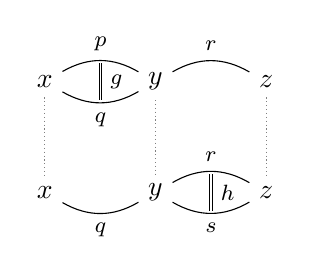
\begin{tikzpicture}[node distance=4em, baseline=(basenode.base)]
      \node[] (x1) {$x$};
      \node[right of=x1] (y1) {$y$};
      \node[right of=y1] (z1) {$z$};
      \node[below of=x1] (x2) {$x$};
      \node[right of=x2] (y2) {$y$};
      \node[right of=y2] (z2) {$z$};
      \draw[bend left] (x1) to node[above] (p) {\footnotesize$p$} (y1);
      \draw[bend right] (x1) to  node[below] (q1) {\footnotesize$q$} (y1);
      \draw[bend left] (y1) to node[above] (r1) {\footnotesize$r$} (z1);
      \draw[bend left] (y2) to node[above] (r2) {\footnotesize$r$} (z2);
      \draw[bend right] (y2) to  node[below] (s) {\footnotesize$s$} (z2);
      \draw[bend right] (x2) to node[below] (q2) {\footnotesize$q$} (y2);
      \draw[double, shorten >=.1em, shorten <=.1em] (p) to node[right] {\footnotesize$g$} (q1);
      \draw[double, shorten >=.1em, shorten <=.1em] (r2) to node[right] {\footnotesize$h$} (s);
      \draw[gray,densely dotted] (x1) to node (basenode){} (x2) (y1) to (y2) (z1) to (z2);
    \end{tikzpicture}%
    =%
    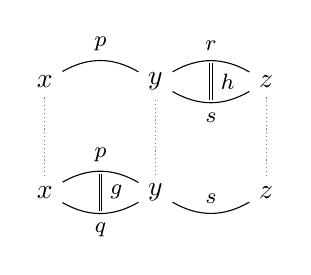
\begin{tikzpicture}[node distance=4em, baseline=(basenode.base)]
      \node[] (x1) {$x$};
      \node[right of=x1] (y1) {$y$};
      \node[right of=y1] (z1) {$z$};
      \node[below of=x1] (x2) {$x$};
      \node[right of=x2] (y2) {$y$};
      \node[right of=y2] (z2) {$z$};
      \draw[bend left] (x2) to node[above] (p) {\footnotesize$p$} (y2);
      \draw[bend right] (x2) to  node[below] (q1) {\footnotesize$q$} (y2);
      \draw[bend right] (y2) to node[above] (r1) {\footnotesize$s$} (z2);
      \draw[bend left] (y1) to node[above] (r2) {\footnotesize$r$} (z1);
      \draw[bend right] (y1) to  node[below] (s) {\footnotesize$s$} (z1);
      \draw[bend left] (x1) to node[above] (p2) {\footnotesize$p$} (y1);
      \draw[double, shorten >=.1em, shorten <=.1em] (p) to node[right] {\footnotesize$g$} (q1);
      \draw[double, shorten >=.1em, shorten <=.1em] (r2) to node[right] {\footnotesize$h$} (s);
      \draw[gray,densely dotted] (x1) to node (basenode){} (x2) (y1) to (y2) (z1) to (z2);
    \end{tikzpicture}%
    \caption{%
      Visual representation of~\cref{eq:horizontal-comp}. The vertical
      dotted lines denotes composition.%
    }\label{fig:horizontal-comp}
  \end{marginfigure}%
  This equality takes place in $r\cdot p = s\cdot q$ and is better
  represented by the diagram in~\cref{fig:horizontal-comp}. %
  One prove such a result by induction on $h$. Indeed, when
  $h\jdeq \refl r$, then both sides of the equation reduces through
  path algebra to $\ap {r\cdot\blank} (g)$. Now we are interested in
  this result when $x,y,z$ are all definitionally $a$, and $p,q,r,s$
  are all definitionally $\refl a$. In that case, one has that
  $\ap {\refl a\cdot \blank}$ and $\ap {\blank\cdot\refl a}$ both act
  trivially, and the equation becomes: $h\cdot g = g \cdot h$.

  One still has to prove that the function $\loopspace$ is an inverse
  for $\BB$. Given an abelian group $G$, the proof
  of~\cref{lemma:universal-cover-simply-connected} gives an
  equivalence between $\B\loopspace {(\BB G)}$ and the connected
  component of $\id_{\BG_\div}$ in $\BG_\div=\BG_\div$. By
  definition, this is the classifying type of $\grpcenter(G)$. Being
  abelian, $G$ is isomorphic to its center
  (\cref{def:abelian-groups}), and so it yields an element of
  $\loopspace {(\BB G)} =_{\typegroup} G$. %
  \marginnote[-1.5\baselineskip]{%
    If $X \ptdweq Y$ denote the type of pointed equivalences between
    pointed types $X,Y:\UUp$, then the univalence axiom implies that
    there is an equivalence
    \begin{displaymath}
      (X=Y) \weq (X \ptdweq Y).
    \end{displaymath}%
  }%
  Conversely, take a pointed simply connected $2$-type $(A,a)$. One
  wants to prove $\BB (\loopspace {(A,a)}) \weq_\ast (A,a)$. One
  should first notice that, because $\loopspace (A,a)$ is an abelian
  group,
  \begin{fullwidth}
  \begin{equation}
    \label{eq:loopspace-A-abelian}%
    {\B\loopspace \left( \BB (\loopspace {(A,a)}) \right)}
    \weq \conncomp{((a=a)=(a=a))}{\refl{a=a}} \weq (a=a,\refl a).
  \end{equation}
\end{fullwidth}
  This equivalence maps a path
  \begin{displaymath}
    (p,!):(a=a,\settrunc{\refl{a=a}})=(a=a,\settrunc{\refl{a=a}})
  \end{displaymath}
  to the evaluation $p(\refl a): a=a$.

  %% OLD MATERIAL, can still be useful.
  %%
  % We will now provide
  % \begin{displaymath}
  %   \Phi : \BB {(\loopspace {(A,a)})} \ptdto (A,a)
  % \end{displaymath}
  % such that $\loopspace(\Phi)$ is the previous equivalence.
  % To be able to
  % express $\Phi$, we need a small gadget about truncations of
  % function
  % types: for types $X,Y:\UU$, given an element
  % $f_0:\setTrunc{X\to Y}$, one constructs a map
  % $\lceil f_0 \rceil : \setTrunc X \to \setTrunc Y$; the type of
  % $\lceil f_0 \rceil$ being a set, one might as well suppose that
  % $f_0 \jdeq \settrunc f$ for some $f:X\to Y$; then we set
  % $\lceil f_0 \rceil (\settrunc x) = \settrunc{f(x)}$, which
  % suffices
  % in order to define $\lceil f_0 \rceil$ entirely because its
  % codomain
  % $\setTrunc Y$ is a set. If we assume the axiom of
  % choice\footnote{What is the status of AC in this book??}, then
  % $\lceil \blank \rceil$ is injective when $Y$ is a set.
  %%
  We will now define a pointed map
  $\Phi : (A,a) \ptdto \BB (\loopspace {(A,a)})$, and prove
  subsequently that this is an equivalence. Let $T : A \to \UU$ be the
  type family define by
  \begin{displaymath}
    T(a') \defequi \sum_{\alpha:\setTrunc{(a=a)\weq(a=a')}}
    \prod_{p:a=a'}\alpha=\settrunc {p\cdot\blank}
  \end{displaymath}
  We claim that $T(a')$ is contractible for all $a':A$. By
  connectedness of $A$, it is equivalent to showing that $T(a)$ is
  contractible. However
  \begin{align*}
    T(a)
    &\jdeq \sum_{\alpha:\setTrunc{(a=a)\weq(a=a)}}\prod_{p:a=a}
      \alpha = \settrunc {p\cdot \blank}
    \\
    &\weq \sum_{\alpha:\setTrunc{(a=a)\weq(a=a)}} \alpha = \settrunc{\id_{a=a}}
    \\
    &\weq 1
  \end{align*}
  Let then $\Phi (a')$ be the element
  $(a=a', \kappa_{a'}):\univcover \UU {a=a}$ where $\kappa_{a'}$ is
  the first projection of the center of contraction of $T(a')$. In
  particular, following the chain of equivalences above, $\Phi(a)$ is
  defined as $(a=a, \settrunc{\refl {a=a}})$, hence $\Phi(a)$ is
  trivially pointed by a reflexivity path. To verify that $\Phi$, thus
  defined, is an equivalence, one can use connectedness of
  $\BB(\loopspace (A,a))$ and only check that
  $\inv\Phi(a=a,\settrunc{\refl {a=a}})$ is contractible. However,
  \begin{displaymath}
    \inv\Phi(a=a,\settrunc{\refl {a=a}}) \simeq \sum_{a':A}
    \sum_{\varphi : (a=a) \weq (a=a')}\settrunc{\varphi} = \kappa_{a'}.
  \end{displaymath}
  For an element $a':A$ together with $\varphi: (a=a) \weq (a=a')$
  such that the proposition $\settrunc \varphi = \kappa_{a'}$ holds, a
  path between $(a,\id_{a=a},!)$ and $(a',\varphi,!)$ consists of a
  path $p:a=a'$ and a path $q:(x\mapsto p x) = \varphi$. We have a
  good candidate for $p$, namely $p\defequi \varphi(\refl
  a):a=a'$. However we don't have quite $q$ yet. Consider, for any
  $a':A$, the function
  \begin{fullwidth}
    \begin{displaymath}
      \ev_{\refl a}^{a'} :
      \left(
        (a=a, \settrunc{\refl{a=a}} ) =
        (a=a', \kappa_{a'} )
      \right)
      \to (a=a'),\quad (\psi,!) \mapsto \psi(\refl a) 
    \end{displaymath}
  \end{fullwidth}
  Note that $\ev_{\refl a}^{a}$ is precisely the equivalence
  $\loopspace{(\BB\loopspace(A,a))}\weq (a=a)$ described
  in~\cref{eq:loopspace-A-abelian}. Hence, by connectedness of $A$,
  one gets that the proposition $\isEq(\ev_{\refl a}^{a'})$ holds for
  all $a':A$. In particular, because the propositions
  $\settrunc \varphi = \kappa_{a'}$ and
  $\settrunc {p\cdot\blank} = \kappa_{a'}$ holds, one gets elements
  $(\varphi,!)$ and $(x\mapsto px,!)$ in the domain of
  $\ev_{\refl a}^{a'}$. Their image $\ev_{\refl a}^{a'}(\varphi,!)$
  and $\ev_{\refl a}^{a'}(x\mapsto px,!)$ are both equal to $p$, which
  provides a path $(x\mapsto px,!)=(\varphi,!)$ in the domain. The
  first component is the path $q:(x\mapsto px) = \varphi$ that we
  wanted.
\end{proof}


\section{$G$-sets vs $\abstr(G)$-sets}
\label{sec:Gsetsabstrconcr}

Given a group $G$ it should by now come as no surprise that the type of $G$-sets is equivalent to the type of $\abstr(G)$-sets.

Recall from \cref{def:abstrGtorsors} that the type of $\abstr(G)$-set is
$$Set_{\abstr(G)}^\abstr\defequi \sum_{\mathcal X:\Set}\Hom_\abstr({\abstr(G)},\abstr(\Sigma_{\mathcal X})).$$
According to \cref{lem:homomabstrconcr}
$$\abstr:\Hom(G,\Sigma_{\mathcal X})\to\Hom^\abstr(\abstr(G),\abstr(\Sigma_{\mathcal X}))$$
is an equivalence, where the group $\Sigma_{\mathcal X}$ (as a pointed connected groupoid) is the component of type $\Set$, pointed at $\mathcal X$.  The component information is moot since we're talking about pointed maps from $\BG$ and we see that $\Hom(G,\Sigma_{\mathcal X})$ is equivalent to $\sum_{F:\BG_\div\to\Set}(\mathcal X=F(\sh_G))$.  Finally, 
$$\mathrm{pr}:\sum_{\mathcal X}\sum_{F:\BG_\div\to\Set}(\mathcal X=F(\sh_G))\we 
%\sum_{F:\BG_\div\to\Set}\sum_{\mathcal X}(\mathcal X=F(\sh_G))\we 
(\BG_\div\to\Set),\quad \mathrm{pr}(\mathcal X,F,p)\defequi F
$$
is an equivalence (since $\sum_{\mathcal X}(\mathcal X=F(\sh_G))$ is contractible).  
Backtracking these equivalences we see that we have established
\begin{lemma}
  \label{lem:actionsconcreteandabstract}
  Let $G$ be a group.  Then the map
  $$\ev_{\sh_G}:\GSet\to\Set^\abstr_{\abstr(G)},\qquad \ev_{\sh_G}(X)\defequi(X(\sh_G),a_X)
$$
is an equivalence, where the action $a_X:\Hom^\abstr(\abstr(G), \abstr(\Sigma_{X(\sh_G)}))$ is given by transport $X^=:\USym G\to (X(\sh_G)=X(\sh_G))$.
\end{lemma}
If $X$ is a $G$-set, $g:\USym G$ and $x:X(\sh_G)$, we seek forgiveness for writing $g\cdot x:X(\sh_G)$ instead of $\cast(a_X(g))(x)$.\footnote{and I ask forgiveness for strongly disliking the use of ``$\cast$'' as a name for some tacitly understood map!}

\begin{example}
  \label{ex:abstrandconj}
  Let $H$ and $G$ be groups.  Recall that the set of homomorphisms from $H$ to $G$ is a $G$-set in a natural way:
$$\Hom(H,G):\BG\to\Set,\quad \Hom(H,G)(y)\defequi \sum_{F:\BH_\div\to \BG_\div}(y=F(\sh_H)).$$

What abstract $\abstr(G)$-set does this correspond to?
In particular, under the equivalence $\abstr:\Hom(H,G)\to\Hom^\abstr(\abstr(H),\abstr(G))$, what is the corresponding action of $\abstr(G)$ on the abstract homomorphisms?
%$\Hom^\abstr(\abstr(H),\abstr(G))$?  

The answer is that $g:\USym G$ acts on $\Hom^\abstr(\abstr(H),\abstr(G))$ by postcomposing with conjugation $c^g$ by $g$ as defined in \cref{ex:conjhomo}.  

Let us spell this out in some detail:
If $(F,p):\Hom(H,G)(\sh_G)\defequi
 \sum_{F:\BH_\div\to \BG_\div}(\sh_G=F(\sh_H))$ and $g:\USym G$, then $g\cdot(F,p)\defequi(F,p\,g^{-1})$.  If we show that the action of $g$ sends $\abstr(F,p)$ to $c^g\circ\abstr(F,p)$ we are done.

Recall that $\abstr(F,p)$ consists of the composite 
$$\xymatrix{\USym H\ar[r]^-{F^=}&(F(\sh_H)=F(\sh_G))\ar[rr]^-{t\mapsto p^{-1}t\,p}&&\USym G},$$ 
(\ie $\abstr(F,p)$ applied to $q:\USym H $ is  $p^{-1}F^=(q)\,p$)  together with the proof that this is an abstract group homomorphism.  
We see that $\abstr(F,p\,g^{-1})$ is given by conjugation:
$q\mapsto(p\,g^{-1})^{-1}F^=(q)\,(p\,g^{-1})=g\,(p^{-1}F^=(q)\,p)\,g^{-1}$, or in other words $c^g\circ\abstr(F,p)$.
\end{example}
For reference we list the conclusion of this example as a lemma''
\begin{lemma}\label{lem:abstrandconj}
  If $H$ and $G$ are groups, then the equivalence of \cref{lem:actionsconcreteandabstract} sends the $G$-set $\Hom(H,G)$ to the $\abstr(G)$-set $\Hom^\abstr(\abstr(H),\abstr(G))$ with action given by postcomposing with conjugation by elements of $\abstr(G)$.
\end{lemma}

If $f:\Hom(G,G')$ is a homomorphism, then precomposition with $\Bf:\BG\to \BG'$ defines a map $$f^*:(G'\text{-}\Set)\to(G\text{-}\Set).$$
We will have the occasion to use the following result which essentially says that if $f:\Hom(G,G')$ is a ``surjective homomorphism'', then $f^*$ embeds the type of $G'$-sets as some of the components of the type of $G$-sets.
\begin{lemma}
  \label{lem:epifullyfaithful}
  Let $G$ and $G'$ be groups and let $f:\Hom(G,G')$ be a homomorphism.  If the induced map $f:\USym G\to\USym {G'}$ is surjective (\cf \cref{def:injection}), then the map $f^*:(G'\text{-}\Set)\to(G\text{-}\Set)$ (induced by precomposition with $\Bf:\BG\to \BG'$) is ``fully faithful'' in the sense that if $X,Y$ are $G'$-sets, then
$$f^*:(X=Y)\to(f^*X=f^*Y)
$$
is an equivalence.
\end{lemma}
\begin{proof}
  Evaluation at $\sh_G$  yields an injective map 
$$\mathrm{ev}_{\sh_G}:(f^*X=f^*Y)\to(X(f(\sh_G)=Y(f(\sh_G)))$$ and the composite 
$$\mathrm{ev}_{\sh_G}f^*=\mathrm{ev}_{f(\sh_G)}:(X=Y)\to(X(f(\sh_G)=Y(f(\sh_G)))$$
 is the likewise injective, so $f^*:(X=Y)\to(f^*X=f^*Y)$ is injective. 

For surjectivity, let $F':f^*X=f^*Y$ and write, for typographical convenience, $a:X(f(\sh_G)=Y(f(\sh_G))$ for $\mathrm{ev}_{\sh_G}F'\defequi F'_{\sh_G}$.  
By the equivalence between $G$-sets and $\abstr(G)$-sets, $F'$ is uniquely pinned down by $a$ and the requirement that for all $g'=f(g)$ with $g:\USym G$ the diagram 
$$\xymatrix{X(f(\sh_G))\ar@{=}[r]^{X({g'})}\ar@{=}[d]_{a}&
  X(f(\sh_G))\ar@{=}[d]_{a}\\
  Y(f(\sh_G))\ar@{=}[r]^{Y({g'})}&Y(f(\sh_G))}
$$
commutes.  Likewise, (using transport along the identity $p_f:\sh_{G'}=f(\sh_G)$) an $F:X=Y$ in the preimage of $a$ is pinned down by the commutativity of the same diagram, but with $g':f(\sh_G)=f(\sh_G)$ arbitrary (an a priori more severe requirement, again reflecting injectivity).   However, when $f:\USym G\to\USym {G'}$ is surjective these requirements coincide, showing that $f^*$ is an equivalence.


% Fix for the moment an  $a:X(f(\sh_G)=Y(f(\sh_G))$

% Now, by transport along the identity $p_f:\sh_{G'}=f(\sh_G)$ and the equivalence between $G'$-sets and $\abstr(G')$-sets, an identity $F':X=Y$ of $G'$-sets is uniquely pinned down by an identity $F'_{f(\sh_G)}:X(f(\sh_G)=Y(f(\sh_G))$ together with the proposition that for all $g':f(\sh_G)=f(\sh_G)$ the diagram $$\xymatrix{X(f(\sh_G))\ar@{=}[r]^{X_{g'}}\ar@{=}[d]_{F'_{f(\sh_G)}}&
%   X(f(\sh_G))\ar@{=}[d]_{F'_{f(\sh_G)}}\\
%   Y(f(\sh_G))\ar@{=}[r]^{Y_{g'}}&Y(f(\sh_G))}
% $$
% commutes.  Likewise, an identity $F:f^*X=f^*Y$ is given by exactly the same data, except that the diagram is only required to commute for $g'=f(g)$ for all $g:\USym G$.  But when $f:\USym G\to\USym {G'}$ these requirements coincide.


% ; $F:X=Y$ is in the preimage of $a:X(f(\sh_G)=Y(f(\sh_G))$ if and only if $a=F_{f(\sh_G)}$ and for all $g':f(\sh_G)=f(\sh_G)$ the diagram
% $$\xymatrix{X(f(\sh_G))\ar@{=}[r]^{X_{g'}}\ar@{=}[d]_{F_{f(\sh_G)}}&
%   X(f(\sh_G))\ar@{=}[d]_{F_{f(\sh_G)}}\\
%   Y(f(\sh_G))\ar@{=}[r]^{Y_{g'}}&Y(f(\sh_G))}
% $$
% commutes.  However, since $f$ is surjective there is a $g:\USym G$ so that $g'=f(g)$.  Therefore, anything in $f^*X=f^*Y$ which is in the preimage of $a$ is in the image of $f^*:X=Y$ and we have shown that $f^*$ is also a surjection.
\end{proof}



\section{Sums of groups}
\label{sec:coprod}
We have seen how the group of integers $\ZZ=(S^1,\base)$ synthesizes the notion of one symmetry with no relations: every symmetry of the circle is of the form $\Sloop^n$ for some unique $n$.  Also, given any group $G=\aut_A(a)$, the set $a=a$ of symmetries of $a$ corresponds to the set of homomorphisms $\ZZ\to G$, \ie to pointed functions $(S^1,\base)\to_*(A,a)$ by evaluation at $\Sloop$.  What happens if we want to study more than one symmetry at the time?  

For instance, is there a group $\ZZ\vee%\boxplus
\ZZ$ so that for any group $G=\aut_A(a)$ a homomorphism $\ZZ\vee%\boxplus
\ZZ\to G$ corresponds to {\bf two} symmetries of $a$?  
At the very least, $\ZZ\vee\ZZ$ itself would have to have two symmetries and these two can't have any relation, since in a general group $G=\aut_A(a)$ there is a priori no telling what the relation between the symmetries of $a$ might be.  
Now, \emph{one} symmetry is given by a pointed function $(S^1,\base)\to_*(A,a)$ and so a \emph{pair} of symmetries is given by a function $f:S^1+S^1\to A$ with the property that $f$ sends each of the base points of the circles to $a$.  But $S^1+S^1$ is not connected, and so not a group.  To fix this we take the clue from the requirement that both the base points were to be sent to a common base point and \emph{define} $S^1\vee S^1$ to be what we get from $S^1+S^1$ when we \emph{insert an identity} between the two basepoints.
$$\xymatrix{\base\ar@(ul,dl)[]|{\Sloop}\ar@{.>}[rr]^{\text{identify!}}&&\base\ar@(ur,dr)[]|{\Sloop}}
$$
The amazing thing is that this works -- an enormous simplification of the classical construction of the ``free products'' or ``amalgamated sum'' of groups.  We need to show that the ``wedge'' $S^1\vee S^1$ is indeed a group, and this proof simultaneously unpacks the classical description.

% \begin{definition}
%   \label{def:wedge}
%   Let $(A_1,a_1)$ and $(A_2,a_2)$ be pointed types.  Their wedge is the pointed type $(A_1\vee A_2,a_{12})$ given as a higher inductive type\footnote{how/where discussed?} by
%   \begin{enumerate}
%   \item functions $i_1:A_1\to A_1\vee A_2$ and $i_2:A_2\to A_1\vee A_2$
%   \item an element $a_{12}: A_1\vee A_2$ (where we point the type),
%   \item identities $g_1:i_1a_1=a_{12}$ and $g_2:i_2a_2=a_{12}$.
%   \end{enumerate}
%   The function 
% $$i^g_1:(a_1=_{A_1}a_1)\to(a_{12}=_{A_1\vee A_2}a_{12})$$ 
% is defined by $i^g_1(p)\defequi g_1i_1(p)g_1^{-1}$, and likewise $i_2^g(q)\defequi g_2i_2(q)g_2^{-1}$.
% \end{definition}
% ((PICTURE))

% \begin{lemma}
%   \label{lem:wedgeofgpoidisgpoid}
%   Let $\aut_{A_1}(a_1)$ and $\aut_{A_2}(a_2)$ be decidable groups, then the wedge sum $\aut_{A_1\vee A_2}(a_{12})$ is a decidable group.
% \end{lemma}
% \begin{proof}
% That ${A_1\vee A_2}$ is connected follows by transitivity of identity, passing through the identities $g_1$ and $g_2$ in the wedge if necessary.

% We must prove that the wedge is a groupoid, \ie that all identity types are sets, which we do by giving an explicit description of the universal \covering.  The idea is that an identity in $a_{12}=x$ can be factored into a string of identities, each lying solely in $A_1$ or in $A_2$.  We define a family of sets consisting of exactly such strings of identities --  it is a set since $A_1$ and $A_2$ are groupoids -- and prove that it is equivalent to the family $P(x)\defequi(a_{12}=_{A_1\vee A_2}x)$ which consequently must be a family of sets.

%   We use the notation of \cref{def:wedge} freely, and for ease of notation, let $a_{2k+i}\defequi a_i$ for $i=1,2$, $k:\NN$.
% Define families of sets
% $$C_i:A_i\to\Set,\qquad i=1,2$$
% by 
% $$C_i(x)\defequi(a_i=_{A_i}x)\times\sum_{n:\NN}\prod_{1\leq k\leq n}\sum_{p_k:a_{i+k}=% _{A_{i+k}}
%   a_{i+k}}(p_k\neq\refl {a_{i+k}})$$
% when $x:A_i$.  Note that $p_k\neq\refl{a_{i+k}}$ makes sense and is a proposition since our groups are decidable; we leave it out when naming elements.  Also, set
% $$C(a_{12})\defequi \sum_{i:\bn 1}(a_i=a_i)\times\sum_{n:\NN}\prod_{1\leq k\leq n}\sum_{p_k:a_{i+k}=% _{A_{i+k}}
%   a_{i+k}}(p_k\neq\refl {a_{i+k}})
% $$
% Define $C(g_i):C_i(a_1)\to C(a_{12})$ by
% $$C(g_i)(p_0,n,p_1\dots,p_n)=
% \begin{cases}
%   (1-i,p_1,n-1,p_2\dots,p_n)& \text{ if }p_0=\refl{a_i}\\
%   (i,\refl{a_i},p_0,n+1,p_1\dots,p_n)& \text{ if }p_0\neq\refl{a_1}.
% \end{cases}
% $$
% $C_{12}$ is ((obviously or write out)) an equivalence, and so the triple $(C_1,C_2,C_{12})$ defines a family
% $$C:A_1\vee A_2\to\Set.$$
% We will show that $C$ is equivalent to $P\defequi \pathsp{a_{12}}$, which is given by $P(x)=(a_{12}=x)$, and so that the identity types of the wedge are sets.

% One way is the ``inclusion''; more precisely, 
% $$\alpha:\prod_{x:A_1\vee A_2}(P(x)\to C(x))$$ is given by letting identities be considered as strings of length zero: $\alpha_i(i_ia)(p)=(0,p):C_i(a)$.  This is well defined since $\alpha_2(i_2a_2)(gpg^{-1})=C_{12}\alpha_1(i_1a_1)(p)$ ((is this how you'd say this?  Feel free to fix.  Remember that $C(x)$ is a set)).
% The other way, 
% $$\beta:\prod_{x:A_1\vee A_2}(C(x)\to P(x)),$$ is given by composing the identities, using the glue $g_1$ and $g_2$ to make their ends meet: $\beta_1(n,p_0,\dots,p_n,!)\defequi i_1(p_0)g^{-1}i_2^g(p_1)i_1^g(p_2) \dots i_{n+1}^g(p_n)$. % (ending in $\dots gi_1(p_n)$ if $n$ is even and $\dots g^{-1}i_2(p_n)g$ if $n$ is odd) 
% and likewise for $\beta_2$ and the glue ((write)).

% That $\beta\alpha(p)=p$ follows by path induction: it is enough to prove it for 
% $p\defequi\refl{}$ ((here the assymmetry of our definition makes saying this slightly awkward since the basepoint is in $i_1A_1$; fix)).  That $\alpha\beta(n,p_0,\dots,p_n)=(n,p_0,\dots,p_n)$ follows by induction on $n$ ((write)).
% \end{proof}

We start by giving a definition of the wedge construction which is important for pointed types in general and then prove that the wedge of two groups is a group whose symmetries are arbitrary ``words'' in the original symmetries.

\begin{definition}
  \label{def:wedge}
  Let $(A_1,a_1)$ and $(A_2,a_2)$ be pointed types.  The \emph{wedge}\index{wedge of pointed types} is the pointed type $(A_1\vee A_2,a_{12})$ given as a higher inductive type\footnote{how/where discussed?} by
  \begin{enumerate}
  \item functions $i_1:A_1\to A_1\vee A_2$ and $i_2:A_2\to A_1\vee A_2$
  \item an identity $g:i_1a_1=i_2a_2$.
  \end{enumerate}
We point this type at $a_{12}\defequi i_1a_1$.
  The function 
$$i^g_2:(a_2=_{A_2}a_2)\to(a_{12}=_{A_1\vee A_2}a_{12})$$ 
is defined by $i^g_2(p)\defequi g^{-1}i_2(p)g$, whereas (for notational consistency only) we set $i_1^g\defequi i_1:(a_1=_{A_1}a_1)\to(a_{12}=_{A_1\vee A_2}a_{12})$.
Simplifying by writing $i:A_1+A_2\to A_1\vee A_2$ for the function given by $i_1$ and $i_2$ (with basepoints systematically left out of the notation), 
the induction principle is
$$\prod_{C:(A_1\vee A_2)\to\UU}\sum_{s:\prod_{a:A_1+A_2}Ci(a)}%\sum_{s_2:\prod_{a:A_2}Ci_2(a)}
((s(a_1)=C(g^{-1})s(a_2))\,\to\,\prod_{x:(A_1\vee A_2)}C(x)).$$
\end{definition}


Unraveling the induction principle we see that if $B$ is a pointed type, then a  pointed function $f:A_1\vee A_2\to_* B$ is given by providing pointed functions $f_1:A_1\to_* B$ and $f_2:A_2\to_* B$  -- the identity $f_1(a_1)=f_2(a_2)$ which seems to be missing is provided by the requirement of the functions being pointed.  For the record
\begin{lemma}
  \label{lem:univvee}
  If $B$ is a pointed type, then the function 
  $$i^*(A_1\vee A_2\to_*B)\to(A_1\to_*B)\times(A_2\to_*B),\qquad i^*(f)=(fi_1,fi_2)
$$
is an equivalence.
\end{lemma}

Here is a picture of $i_2^g(p)$: it is the symmetry of the base point $a_{12}\defequi i_1a_1$ you get by \emph{first} moving to $i_2a_2$ with $g$, \emph{then} travel around with $p$ ($i_2p$, really) and finally go home to the basepoint with the inverse of $g$.
% $$\xymatrix{i_1a_1\ar@/^/[rr]^{g}&&i_2a_2\,\,\,\ar@/^/[ll]^{g^{-1}}\ar@(ur,dr)[]^{p}}
% $$

% $$\xy (-20,20)*+{A};(0,20)*+{B}
% **\crv{}
% \endxy$$
% $$% \xy (-20,20)*+{i_1a_1\,\,};(0,20)*+{}
% % **\crv{}\endxy
% % \xy (0,20)*+{i_2a_2};(0,20)*+{}
% % **\crv{(20,30)&(0,40)&(-20,30)}
% % \endxy
% \xy (-20,20)*+{a_{12}\,\,};(-20,20)*+{}
% **\crv{(10,20)&(-20,35)&(0,45)&(20,35)&(15,20)&(-10,20)}
% %?>*\dir{>}
% ?(.38)*{} *!LD!/^3pt/{>}
% ?(.95)*{} *!LD!/^-15pt/{g^{-1}}
% ?(.03)*{} *!LD!/^-5pt/{g}
% ?(.55)*{} *!LD!/^-7pt/{i_2p}
% \endxy
% $$
% $$\xy (0,20)*+{A};(60,0)*+{B}
% **\crv{(20,20)&(30,20)&(50,-20)&(60,-10)}
%  ?<*\dir{<} ?>*\dir{>}
%  ?(.65)*{\oplus} *!LD!/^-5pt/{x}
%  ?(.65)/12pt/*{\oplus} *!LD!/^-5pt/{x’}
%  ?(.28)*=0{\otimes}-/40pt/*+{Q}="q"
%  +/100pt/*+{P};"q" **\dir{-}
% \endxy
% $$
$$
\xy (-20,20)*+{};(-20,20)*+{}
**\crv{(15,20)&(18,20)&(-10,35)&(10,45)&(25,30)&(20,19)&(0,20)}
%?>*\dir{>}
?(0)*{} *!LD!/^-20pt/{i_1A_1}
?(.45)*{} *!LD!/^2pt/{>}
?(.95)*{} *!LD!/^-15pt/{g^{-1}}
?(.03)*{} *!LD!/^-5pt/{g}
?(.55)*{} *!LD!/^-7pt/{i_2p}
?(.65)*{} *!LD!/^-30pt/{i_2A_2}
?(.87)*{} *!LD!/^-12pt/{i_2a_2}
?(.86)*{} *!LD!/^-2pt/{\bullet}
?(1)*{} *!LD!/^-2pt/{\bullet}
?(1)*{} *!LD!/^-12pt/{a_{12}}
\endxy
$$

We now prove that wedges of decidable groups are decidable groups.   The idea is that an identity in $a_{12}=x$ can be factored into a string of identities, each lying solely in $A_1$ or in $A_2$.  We define a family of sets consisting of exactly such strings of identities --  it is a set since $A_1$ and $A_2$ are groupoids -- and prove that it is equivalent to the family $P(x)\defequi(a_{12}=_{A_1\vee A_2}x)$ which consequently must be a family of sets.
We need to be able to determine whether a symmetry is reflexivity or not, but once we know that, the symmetries of the base point in the wedge are then given by ``words $p_0p_1\dots p_n$'' where the $p_j$ alternate between being symmetries in the first or the second group, and none of the $p_j$ for positive $j$ are allowed to be reflexivity% : effectively a symmetry in the wedge can be decomposed into composites of symmetries in each of the groups
.  Note that there order of the $p_j$s is not negotiable: if I shuffle them I get a new symmetry.
\begin{lemma}
  \label{lem:wedgeofgpoidisgpoid}
  Let $\aut_{A_1}(a_1)$ and $\aut_{A_2}(a_2)$ be decidable groups, then the wedge sum $\aut_{A_1\vee A_2}(a_{12})$ is a decidable group.  

Let $C_1$ be the set of strings $(p_0,n,p_1,\dots,p_n)$ with $n:\NN$ and, for $0\leq j\leq n$ 
\begin{itemize}
\item $p_{j}:a_1=a_1$ for even $j$ 
\item $p_{j}:a_2=a_2$ for odd $j$ and 
\item $p_j$ is not reflexivity for $j$ positive (makes sense and is a proposition since our groups are decidable).
\end{itemize}
  Then the function given by composition in $a_{12}=a_{12}$
$$\beta:C_1\to(a_{12}=a_{12}),\qquad\beta(p_0,n,p_1,\dots p_n)\defequi i_1^gp_0i_2^gp_1i_1^gp_2\dots i_?^gp_n$$ 
(where $i_?^gp_n$  is $i_1^gp_n$ or $i_2^gp_n$ according to whether $n$ is even or odd) is an equivalence.
\end{lemma}
\begin{proof}
That the wedge is connected follows by transitivity of identity, if necessary passing through the identity $g:i_1a_1=i_2a_2$ in the wedge.

We must prove that the wedge is a groupoid, \ie that all identity types are sets, which we do by giving an explicit description of the universal \covering. 

 We use the notation of \cref{def:wedge} freely, and for ease of notation, let $a_{2k+i}\defequi a_i$ and $i_{2k+i}^g\defequi i_i^g$ for $i=1,2$, $k:\NN$.  % Let $i_1:A_1\to A_1\vee A_2$ and $i_2:A_2\to A_1\vee A_2$ be the two inclusions, let $g:i_1\pt_{A_1}=i_2\pt_{A_2}$ be the imposed identity in the (non-symmetric formulation of the) wedge sum based in $\pt_{A_1\vee A_2}\defequi i_1\pt_{A_1}$.  For ease of notation, let $a_{2k+i}$ denote $\pt_{A_i}$ for $i=1,2$, $k:\NN$.
Define families of sets
$$C_i:A_i\to\Set,\qquad i=1,2$$
by 
$$C_i(x)\defequi(a_i=_{A_i}x)\times\sum_{n:\NN}\prod_{1\leq k\leq n}\sum_{p_k:a_{i+k}=% _{A_{i+k}}
  a_{i+k}}(p_k\neq\refl {a_{i+k}})$$
when $x:A_i$.  Note that $p_k\neq\refl{a_{i+k}}$  is a proposition; we leave it out when naming elements. Hence, an element in $C_1(a)$ is a tuple
$(p_0,n,p_1,\dots,p_n)$ where $p_0:a_1=_{A_1}a$, $p_1:a_2=_{A_2}a_2$, $p_2:a_1=_{A_1}a_1$, and so on -- alternating between symmetries of $a_1$ and $a_2$, and where $p_0$ is the only identity allowed to be $\refl{}$. Define $C_{12}:C_1(a_1)\to C_2(a_2)$ by
$$C_{12}(p_0,n,p_1\dots,p_n)=
\begin{cases}
  (\refl{a_2}0,)&\text{ if }p_0=\refl{a_1}, n=0,\\
  (p_1,n-1,p_2\dots,p_n)& \text{ if }p_0=\refl{a_1},n\neq0,\\
  (\refl{a_2},n+1,p_0,\dots,p_n)& \text{ if }p_0\neq\refl{a_1}.
\end{cases}
$$
It is perhaps instructive to see a table of the values $C_{12}(p_0,n,p_1,\dots,p_n)$ for $n<3$:
\begin{center}
  \begin{tabular}{r|c cc}
    &$(p_0,0)$&$(p_0,1,p_1)$&$(p_0,2,p_1,p_2)$\\
    \hline
    $p_0=\refl{a_1}$&$(\refl{a_2},0)$&$(p_1,0)$&$(p_1,1,p_2)$\\
    $p_0\neq\refl{a_1}$&$(\refl{a_2},1,p_0)$&$(\refl{a_2},2,p_0,p_1)$&$(\refl{a_2},3,p_0,p_1,p_2)$
  \end{tabular}
\end{center}
Since $C_{12}$ is an equivalence, the triple $(C_1,C_2,C_{12})$ defines a family
$$C:A_1\vee A_2\to\Set.$$
In particular, $C(a_{12})\defequi C_1(a_1)$.
For $x:A_1$ we let $i^C_1:C_1(x)\to C(i_1(x))$ be the induced equivalence, and likewise for $i^C_2$.
We will show that $C$ is equivalent to $P\defequi \pathsp{a_{12}}$, where $P(x)\defequi(a_{12}=x)$, and so that the identity types in the wedge are equal to the sets provided by $C$.

One direction is by transport in $C$; more precisely, 
$$\alpha:\prod_{x:A_1\vee A_2}(P(x)\to C(x))$$ is given by transport with $\alpha(a_{12})(\refl{a_{12}})\defequi(\refl{a_{1}},0):C(a_{12})$.  %This is well defined since $\alpha_2(i_2\pt_{A_2})(gpg^{-1})=C_{12}\alpha_1(i_1\pt_{A_1})(p)$ ((is this how you'd say this?)).
The other way, 
$$\beta:\prod_{x:A_1\vee A_2}(C(x)\to P(x))$$ is given by composing identities, using the glue $g$ to make their ends meet: 
$$\beta(i_1a)(p_0,n,p_1,\dots,p_n)\defequi i_1(p_0)i_2^g(p_1)i_3^g(p_2) \dots i_{n+1}^g(p_n)$$ 
(here the definition $\dots i_3^g\defequi i_1^g\defequi i_1$ proves handy since we don't need to distinguish the odd and even cases)  % (ending in $\dots gi_1(p_n)$ if $n$ is even and $\dots g^{-1}i_2(p_n)g$ if $n$ is odd) 
and likewise 
$$\beta(i_2a)(p_0,n,p_1,\dots,p_n)\defequi i_2(p_0)g\,i_1^g(p_1)i_2^g(p_2) \dots i_{n}^g(p_n)$$ and compatibility with the glue $C_{12}$ is clear since the composite $\refl{x}p$ is equal to $p$.
%$\beta_1(p_0,n,p_1,\dots,p_n,!)\defequi i_1(p_0)g^{-1}i_2(p_1)gi_1(p_2) g^{-1}\dots $ (ending in $\dots gi_1(p_n)$ if $n$ is even and $\dots g^{-1}i_2(p_n)g$ if $n$ is odd) and likewise for $\beta_2$ and the glue ((write)).

For notational convenience, we hide the $x$ in $\alpha(x)(p)$ and $\beta(x)(p)$ from now on.

That $\beta\alpha(p)=p$ follows by path induction: it is enough to prove it for $x=a_{12}$ and
$p\defequi\refl{a_{12}}$:
$$\beta\alpha(\refl{a_{12}})=\beta(\refl{a_1},0)=i_1^g\refl{a_1}=\refl{a_{12}}.$$  

That $\alpha\beta(p_0,n,p_1\dots,p_n)=(p_0,n,p_1,\dots,p_n)$ follows by induction on $n$ and $p_0$.  For $n=0$ it is enough to consider  $x=a_{12}$ and $p_0=\refl{a_1}$, and then 
$\alpha\beta(\refl{a_1},0)\defequi\alpha(\refl{a_{12}})\defequi(\refl{a_1},0)$.  In general, (for $n>0$) 
\begin{align*}
  \alpha\beta(p_0,n,p_1\dots,p_n)
=&\trp[C]{i_1(p_0)i_2^g(p_1)i_1^g(p_2) \dots i_{n+1}^g(p_n)}(\refl{a_1,0})\\
=&\trp[C]{i_1(p_0)}\dots\trp[C]{i_{n+1}^g(p_n)}(\refl{a_1,0}).
\end{align*}
  The induction step is as follows: let $0< k\leq n$, then 
\begin{align*}
  &\trp[C]{i_k^gp_{k-1}}i^C_{k-1}(p_k,n-k-1,p_{k+1},\dots,p_n)\\
  =&\trp[C]{i_k^gp_{k-1}}i^C_k(\refl{a_{k-1}},n-k,p_k,\dots,p_n)\\
  =&i^C_k\trp[C_k]{p_{k-1}}(\refl{a_{k-1}},n-k,p_k,\dots,p_n)\\
  =&(p_{k-1},n-k,p_k,\dots,p_n).
\end{align*}
((please see whether this makes sense to anybody but yvt))
\end{proof}

\begin{definition}
  \label{def:sumofgroup}
  If $G_1=\aut_{A_1}(a_1)$ and $G_1=\aut_{A_1}(a_1)$ are groups, then their \emph{sum}\index{sum of groups} is defined as
  $$G_1\vee G_2\defequi \aut_{A_1\vee A_2}(a_{12}).$$ The homomorphisms $i_1:G_1\to G_1\vee G_2$ and $i_2:G_2\to G_1\vee G_2$ induced from the structure maps  $i_1:A_1\to A_1\vee A_2$ and  $i_2:A_2\to A_1\vee A_2$ are also referred to as structure maps.
\end{definition}
\begin{lemma}
  \label{lem:sumofgroupsISsum} If $G_1$, $G_2$ and $G$ are groups, then the function
  $$\Hom(G_1\vee G_2,G)\to\Hom(G_1,G)\times\Hom(G_2,G)$$ 
given by restriction along the structure maps is an equivalence.
\end{lemma}
\begin{proof}
  ((write))
\end{proof}
Specializing, we return to our initial motivation and see that mapping out of a wedge of two circles \emph{exactly} captures the information of two independent symmetries:
\begin{corollary}
  \label{cor:ZplusZuniv}
  If $G$ is a group, then the functions
  $$\Hom(\ZZ\vee\ZZ,G)\to \Hom(\ZZ,G)\times\Hom(\ZZ,G)\to G\times G$$
  are equivalences.((fix language))
\end{corollary}
\begin{xca}
This leads to the following characterization of abelian groups formulated purely in terms of pointed connected groupoids (no reference to the identity types).
  \label{xca:whatAREabeliangroups}
  A group $G$ is abelian if and only if the canonical map 
$$+:G\vee G\to G$$ 
(given via \cref{lem:sumofgroupsISsum} by $G\oldequiv G$) extends over the inclusion 
$$i:G\vee G\to G\times G$$ 
(given by the inclusions $\mathrm{in}_1,\mathrm{in}_2:G\to G\times G$).\footnote{I haven't written out a formalization myself}
\end{xca}



% %\section{structure of identity types}
% %\section{automorphism 1-group = fundamental group (hint at higher groups)}
% %\section{homomorphisms induced by functions (early)}
% \section{``more examples: symmetric groups, integers, cyclic groups and modular arithmetic''}
% \section{``group actions, orbits and fixed points''}

% \section{Subgroups}
% \label{sec:subgroups}
% In our discussion of the group $\ZZ=\aut_{S^1}(\base)$ of integers in we discovered that the ``subsymmetries'' formed a very organized structure.  For each natural number $n$ we obtained a set of subsymmetry the entire identity type $\base=\base$, namely the set of all the iterates $(\Sloop^{n})^m$ where $m$ varies over the integers.  When $n$ was positive this was realized as the $n$-fold \covering of $S^1$ , when $n=0$ this was given by the universal \covering.  

% For other groups the ``subsymmetries'' form more involved structures.  One thing is that our concept of a subtype of $B$ is merely the first projection $\sum_{b:B}P(b)\to B$, where the $P$ is a family of propositions.  Another thing is that for group the ``sub'' refers to the associated abstract groups, so that ``$\BH$ is a subgroup of $\BG$'' should \emph{not} mean that ``$\BH$ is a subtype of $\BG$'', but that we have a group homomorphism $f:\Hom(H,G)$ so that the induced function $\USym H\to\USym G$ is an ``inclusion of a subset''. 

% Now, as we've seen, that   $f:\USym H\to\USym G$ is an injection (preimages are propositions) is equivalent to the preimages of $\Bf:\BH\to \BG$ being sets.  Hence we get the following neat formulation.
%     \begin{definition}
%       \label{def:subgroup}
%       Let $G$ be a group.  
%       The \emph{type of subgroups of $G$}\index{type!subgroup} is the type
%       $$\typesubgroup_G\defequi\sum_{H:\typegroup}\sum_{f:\Hom(H,G)}\isset(\Bf^{-1}(\sh_G)).$$
%        A subgroup $(H,f,!)$ is
%       \begin{enumerate}
%       \item \emph{trivial}\index{trivial subgroup} if $\BH$ is contractible
%       \item \emph{proper}\index{proper subgroup} if $\Bf$ is not an equivalence.
%       \end{enumerate}
%     \end{definition}
%     \begin{remark}
%       \label{rem:notationsubgroup}
%       A note on notation is in order.  
% If $(H,i,!)$ is a subgroup of a group $G$ tradition often permits us to relax the burden of notation; we may write ``a subgroup $i:H\subseteq G$'', or, if we don't need the name of $i:\Hom(H,G)$ in what follows, simply ``a subgroup $H\subseteq G$'' or ``a subgroup $H$ of $G$''.
%     \end{remark}

% \begin{lemma}
%   \label{lem:setofsubgroups}
%   If $G$ is a group, then the type $\typesubgroup_G$ of subgroups is a set.
% \end{lemma}
% \begin{proof}
% An identity between two subgroups $i_H:H\subseteq G$ and $i_{H'}:H'\subseteq G$ is an identity $p:H'=_{\typegroup}H$ such that $i_{H'}=i_H\,p$ (a proposition since $\Hom(H',G)$ is a set).
%   By univalence and \cref{lem:eqofconntypes}, the identity type $H=H'$ is equivalent to the set 
% $$\sum_{f:\Hom(H,H')}\isEq(f^=:\USym H\to\USym {H'}).$$  
% %If $(H,i_H,!)$ is a subgroup of $G$, then
% Consequently, the identity type
% $(H,i_H,!)=_{\typesubgroup_G}(H,i_H,!)$ is equivalent to the type of homomorphisms $f:\Hom(H,H)$ which are such that $!:i_H^==i_H^=f^=$ and such that $f^=$ is an equivalence (as we see in a moment this last requirement is redundant).  
% Now, since $(H,i_H,!)$ is a subgroup, $i_H^=$ is an injection of sets, which forces $!:f^==\refl{\USym H}$, which ultimately forces $f$ to be (identical to) the identity homomorphism. 
% \end{proof}
% Not only is the type of subgroups  of $G$ a set, it is in a natural way (equivalent to the value at $\sh_G$ of) a $G$-set which we denote by the same name
% $$%\typesubgroup_G:\BG\to\Set,\qquad 
% \typesubgroup_G(y)\defequi \sum_{H:\typegroup}\sum_{f:\Hom(H,G)(y)}\isset(\Bf^{-1}(\sh_G)),$$
% where  as in \cref{ex:HomHGasGset}  
% $$\Hom(H,G)(y)\defequi\sum_{F:\BH_\div\to \BG_\div}(y=F(\sh_H))$$
% is the $G$-set of homomorphisms from $H$ to $G$.
% % In this interpretation, $(H,F,p,!):\typesubgroup_G(\sh_G)$ represents a subgroup of $G$ (so that $p:\sh_G=F(\sh_H)$).  An identity $g:\USym G$ acts on $\typesubgroup_G(\sh_G)$ by sending $(H,F,p,!)$ to $(H,F,p\,g^{-1},!)$.

% \begin{definition}
%   \label{def:conjactonsubgroups}
%   If $G$ is a group, then the action of $G$ on the set of subgroups is called \emph{conjugation}. 


%   \label{def:conjugate}
%   If $(H,F,p,!):\typesubgroup_G(\sh_G)$ is a subgroup of $G$ and $g:\USym G$, then the subgroups  $(H,F,p,!),(H,F,p\,g^{-1},!):\typesubgroup_G(\sh_G)$ are said to be \emph{conjugate}\index{conjugate}. 
% \end{definition}
% \begin{remark}
%   \label{rem:whyconjugate}
%   The term ``conjugation'' may seem confusing as the %(abstract) 
% action of $g:\USym G$ on a subgroup $(H,F,p,!):\typesubgroup_G(\sh_G)$ (where $p:x=F(\sh_H)$) is simply $(H,F,p\,g^{-1},!)$, which does not seem much like conjugation.  
% However, as we saw in \cref{ex:abstrandconj}, under the equivalence $\abstr:\Hom(H,G)\we\Hom^\abstr(\abstr(H),\abstr(G))$, the corresponding action on $\Hom^\abstr(\abstr(H),\abstr(G))$ is exactly (postcomposition with) conjugation $c^g:\abstr(G)=\abstr(G)$.  
% \footnote{The same phenomenon appeared in \cref{xca:HomZGvsAdG} where we gave an equivalence between the $G$-sets $\Hom(\ZZ,G)$ and $\Ad_G$ (where the action is very visibly by conjugation).}
% % \end{remark}

% % \begin{remark}
%   \label{rem:conjactiononsubgroups}
%  %  It is worthwhile to study this action a bit further.  Let $(H,f,!)$ be a subgroup of $G$ and let $g:\USym G$.  We can trade $f$ for $\abstr(f):\Hom^\abstr(\abstr(G),\abstr(H))$ whose underlying set map is the injection $\Bf^=:\USym H\to\USym G$. %We allow ourselves to write ``$f$'' instead of $\Bf^=$. 
% % As we saw in \cref{ex:abstrandconj}, the action of $g$ postcomposes with conjugation $c^g:\USym G=\USym G$.
% % Hence, if we represent a subgroup as 
% % $$(H,\phi,!):\sum_{H:\typegroup}\sum_{\phi:\Hom^\abstr(\abstr(H),\abstr(G))}\isprop(\phi^{-1}(e_G)),$$ then
% % $g\cdot(H,\phi,!)=(H,c^g\,\phi,!)$.

% % Now, if $g$ comes from $H$, say, $\i_H(h)$
% \end{remark}
% Summing up the remark:
% \begin{lemma}
%   \label{lem:conjugationabstractly}
%   Under the equivalence of \cref{lem:actionsconcreteandabstract} between $G$-sets and $\abstr(G)$-sets, the $G$-set $\typesubgroup_G$ corresponds to the $\abstr(G)$-set
% $$\sum_{H:\typegroup}\sum_{\phi:\Hom^\abstr(\abstr(H),\abstr(G))}\isprop(\phi^{-1}(e_G))$$ of abstract subgroups of $\abstr(G)$, with action $g\cdot(H,\phi,!)\defequi(H,c^g\,\phi,!)$ for $g:\abstr(G)$, where  $c^g:\abstr(G)=\abstr(G)$ is conjugation as defined in \cref{ex:conjhomo}.
% \end{lemma}


% \begin{remark}
%   If you're familiar with the set-theoretic flavor of things, you know that it is important to distinguish between subgroups and injective group homomorphisms.  
% Our use of ``subgroup'' can be defended as follows.  
% It corresponds in set-theoretic language to saying that a subgroup is an injective homomorphism \emph{modulo} the relation forcing that precomposing with an isomorphism yields identical subgroups.  
% Set-theory offers the luxury of having a representative in every equivalence class: namely the image of the injection, type theory does not.
% \end{remark}

% \sususe{The geometry of subgroups: some small examples}
% \label{smallsubgpex}

% As a teaser, and in order to get a geometric feel for the subgroups and their intricate interplay, it can be useful to have some fairly manageable examples to stare at.  
% Some of the main tools for analyzing the geometry of subgroups are collected in \cref{sec:fingp} on finite groups, and we hope the reader will be intrigued by our mysterious claims and go on to study \cref{sec:fingp}.
% That said, the examples we'll present are possible to muddle through by hand without any fancy machinery, but brute force is generally not an option and even for the present examples it is not something you want to show publicly.

% When presenting the subgroups of a group $G$, three types are especially revealing: the set of subgroups $\typesubgroup_G(\sh_G)$, the \emph{groupoid of subgroups} $\typesubgroup(G)\defequi\sum_{y:\BG}\typesubgroup_G(y)$ and what we for now call the ``set of normal subgroups'' $\prod_{y:\BG}\typesubgroup_G(y)$.   Our local use of ``normal subgroup'' is equivalent to the official definition to come.  

% The first projection $\typesubgroup(G)\to \BG$ is referred to as the \emph{\covering of subgroups}.

% \footnote{Write out and fix the concrete examples (cyclic groups and $\Sigma_3$) commented out}
% % \begin{remark}
% % In  \cref{cha:circle} we studied the subgroups of the group of integers $G=\ZZ$ through \coverings over the circle $S^1$ (which we showed was equivalent to $B\ZZ$).
% % We discovered a subgroup $n\ZZ$ for each natural number $n:\NN$ and in the groupoid $\typesubgroup({\ZZ})$ these sit as elements in separate components.  Each of these components are contractible (because addition is commutative: $\ZZ$ is an abelian group).

% % In general, a component $K$ of the groupoid $\sum_{y:\BG}\typesubgroup_G(y)$ of subgroups of a group $G$ may be much more interesting. For one thing the, $K$ can contain many subgroups in the sense that the preimage of the first projection $K\to \BG$ is a set that may have many different elements; each representing a subgroup.  However, this set of subgroup will be a \emph{conjugacy class} of subgroups: the different subgroups are related by the conjugation action of $G$.  

% % If $G$ is abelian this action is trivial, and $\sum_{y:\BG}\typesubgroup_G(y)$ consists of contractible components indexed over the subgroups of $G$.  Otherwise different subgroups may live in the same component of the groupoid of subgroups -- we'll see examples in a moment.

% % In addition, the components will not in general be contractible, revealing the symmetries of the subgroups under the conjugation action.
% % \end{remark}


% % \begin{example}
% %   The trivial group only has itself as a subgroup; the groupoid of subgroups and the set of normal subgroups are singletons.
% % \end{example}
% % \begin{example}
% %   The cyclic group $C_p$ of prime order $p$ has only two subgroups, the trivial and the full subgroup itself and both are normal.  In fact, all subgroups of abelian groups are normal.  

% % In general, the cyclic group $C_n$ of order $n$ has exactly one subgroup for each divisor $i$ of $n$.
% % \end{example}


% % \begin{example}
% %   The group $C_2\times C_2$ has has no less than five subgroups: the trivial one, three subgroups that as groups (as opposed as \emph{sub}groups) are equivalent to $C_2$ and the full group $C_4$ itself.
% % \end{example}
% % \begin{remark}
% %   The permutation group $\Sigma_3$ has four nontrivial proper subgroups.  Three conjugate subgroups isomorphic as groups to $C_2$ and one normal one which is as a group is isomorphic to $C_3$.  The component containing the copies of $C_2$ is equivalent to a circle.
% % \end{remark}
% \sususe{Kernels and cokernels}
% \label{subsec:ker}
% %\newcommand{\ker}{\mathrm{ker}}
% If $\phi:\Hom^\abstr(\mathcal G,\mathcal G')$ is an abstract group homomorphism, the preimage $\phi^{-1}(e_G)$ is a classically called the kernel of $\phi$ and the cokernel is the quotient set of $\mathcal G'$ by the relation that if $g:\mathcal G$ and $g':\mathcal G'$, then $g'\sim g'\cdot\phi(g)$.  
% In our setup with a group homomorphism 
% $$f:\Hom(G,G')\defequi(\BG\to_*\BG'),$$ the kernel and cokernel are just two aspects of the preimage 
% $$(\Bf)^{-1}(\sh_{G'})\defequi\sum_{z:\BG}(\sh_{G'}=\Bf(z)):$$
%  the cokernel is the set of components and the kernel is a preferred component.  This point of view makes it clear that the kernel is a subgroup whereas there is no particular reason for the cokernel to be more than a ($G'$-) set.
% \newcommand{\coker}{\mathrm{coker}\,}
% \newcommand{\image}{\mathrm{im}\,}
% \begin{definition}
%   \label{def:cokernel}
%   Let $f:\Hom(G,G')\defequi(\BG\to_*\BG')$  be a homomorphism. %  The preimage $$f^{-1}(\sh_{G'})\defequi\sum_{z:\BG}(\sh_{G'}=f(z))$$
% % is a groupoid containing important information about $f$.
% The \emph{cokernel}\index{cokernel} of $f$ is the $G'$-set
% $$\coker f:\BG'\to\Set,\qquad \coker f(z)\defequi  \Trunc{(\Bf)^{-1}(z)}_0.\footnote{set trunctation} $$ 
% The associated $\abstr(G')$-set $\coker f(\sh_{G'})$ is also referred to as the cokernel of $f$.  If $f:\Hom(G,G')$ is clear from the context and displays $G$ as a subgroup of $G'$, we often write $G'/G$ for the cokernel of $f$.  

% \end{definition}
% \begin{definition}
%   \label{def:kernel}
% Let $f:\Hom(G,G')$  be a homomorphism.
% Consider the element 
% $$\sh_{\ker f}\defequi(\sh_G,p_f):(\Bf)^{-1}(\sh_{G'})$$ (where $p_f:\sh_{G'}=\Bf(\sh_G)$ is the part of $f$ claiming it is a pointed map). 
% Define the \emph{kernel}\index{kernel}  of $f$ to be the group defined by the pointed component  of $\sh_{\ker f}$ in $(\Bf)^{-1}(\sh_{G'})$:
% $$\ker f\defequi ((\Bf)^{-1}(\sh_{G'})_{(\sh_{\ker f})},\sh_{\ker f}).
% $$ 
% Written out,
% $B\ker f_\div\defequi \sum_{z:\BG}\sum_{p:\sh_{G'}=f(z)}\Trunc{\sh_{\ker f}=(z,p)}.$  

% The first projection $\Bker f\to_* \BG$ displays the kernel $\ker f$ as a subgroup of $G$ (\emph{sub}group since the preimages are equivalent to the sets $\sum_{p:\sh_{G'}=\Bf(z)}\Trunc{\sh_{\ker f}=(z,p)}$).  

% A subgroup is said to be \emph{normal}\index{normal} if it is the kernel of a surjective homomorphism.\footnote{clarify the relation between the surjective homomorphism and the subgroup}
% \end{definition}

% \begin{definition}
% \label{def:image}\label{def:surjective}
% The \emph{image}\index{image} of $f$ is the subgroup of $G'$ given by $B\image f\defequi \sum_{z:\BG'}\coker f(z)$ pointed at $\pt_{\image f}\defequi (\sh_{G'},|\sh_G,p_f|)$ together with the first projection $B\image f\to \BG'$ (plus the fact that $\coker f(z)$ is a set).  

% The \emph{induced homomorphism} $\tilde f:\Hom(G,\image f)$ is given by sending $x:\BG$ to 
% $$B\tilde f(x)\defequi (\Bf(x),|x,\refl{\Bf(x)}|).$$ 

% We say that the homomorphism $f$ is \emph{surjective}\index{surjective! group homomorphism} if $(\Bf)^{-1}(\sh_{G'})$ is connected.
% %, or equivalently if $\image f\to G'$ is an equivalence.
% \end{definition}
% % \begin{remark}
% %   \label{rem:cokerasGset}
% %   If $f:\Hom(G,G')$ we notice that the abstract group $\abstr(G')$ acts on $\coker(f)\defequi\Trunc{f^{-1}(\sh_{G'})}_0$, making the cokernel an $\abstr(G')$-set.  If we prefer to talk about a $G'$-set, we consider the cokernel as the set-family $$BG'\to\Set,\qquad z\mapsto   \Trunc{f^{-1}(z)}_0.$$  
% % We will see this used most frequently when considerint inclusions of subgroups: if $H$ is a subgroup of $G$, then $G/H$ is a $G$-set.
% % \end{remark}
% In view of \cref{ex:charsurinj} below, the families  
% $$\mathrm{issurj},\mathrm{isinj}:\Hom(G,G')\to\Prop
% $$
% of propositions that a given homomorphism is surjective or injective have several useful interpretations.
% \begin{xca}
%   \label{ex:charsurinj}
%   Let $f:\Hom(G,G')$ Prove that
%   \begin{enumerate}
%   \item the following are equivalent
%     \begin{enumerate}
%     \item $f$ is a surjective homomorphism (\cref{def:surjective}),
%     \item the cokernel of $f$ is contractible,
%     \item the first projection $B\image f\to BG$ is an equivalence
%     \item the induced map of sets 
% $f^=:\USym G\to\USym {G'}$ is a surjection
%     \end{enumerate}
%   \item the following are equivalent
%     \begin{enumerate}
%     \item $f$ is an injective homomorphism (\ie the induced map of sets 
% $f^=:\USym G\to(\sh_{G'}\to\sh_{G'})$
% is an injection)
% \item the kernel of $f$ is trivial
% \item $Bf:BG\to BG'$ is a \covering.
% \item the induced map $B\tilde f:BG\to B\image f$ is an equivalence.
%     \end{enumerate}
%   \end{enumerate}
% \end{xca}



% Note that if $f:\Hom(G,G')$, then the composite of the induced homomorphism $\tilde f:\Hom(G,\image f)$ with the subgroup inclusion (first projection) of $\image f$ in $G'$ is $f$ by definition.  We will refer to this as the \emph{factorization of $f$ through its image}.

% \begin{lemma}
%   \label{lem:kerandcoker}
%   \label{lem:countinggps}
%   Let $f:\Hom(G,G')$ be a group homomorphism.  The induced homomorphism $\tilde f:\Hom(G,\image f)$ is a surjective homomorphims and $f$ factors as $\tilde f$ followed by the inclusion of the image of $f$ in $G'$.  The induced map $(B\tilde f)^{-1}(\pt_{\image f})\to (Bf)^{-1}(\sh_{G'})$ induces an equivalence $B\ker\tilde f\simeq B\ker f$.
% \end{lemma}
% \begin{proof}
% Only the last part needs further comment, but follows since since for $x:BG$ the first projection from $\pt_{\image f}=(Bf,|x,\refl{Bfx}|)$ to $\sh_{G'}=f(x)$ is an equivalence (the fibers are true propositions).
%   \footnote{\color{blue}  
%  Also show counting results for the finite group part somewhere.} 
% \end{proof}

% Finally, the image factorization would have been useless were it not for the fact that it is unique:
% \begin{lemma}
%   \label{lem:uniquenessofimagefactorizationforgroups}
%   Let $G,H,G'$ be groups, let $h:\Hom(G,H)$ and $j:\Hom(H,G')$ be homomorphisms and let $!:f=j\,h$.  If $h$ is surjective there is a unique homomorphism $t:\Hom(H,\image f)$ so that $\tilde f=t\, h$ and $j$ is $t$ composed with the first projection from $\image f$ to $ G'$.
% \end{lemma}
% \begin{proof}
%   We've used that we're operating with groupoids to simplify the statement, but a similar statement follows generally by essentially the proof below if you keep track of the element in $f=j\,h$.  To simplify we drop the ``$B$''s from the notation, writing ``$f$'' instead of ``$Bf$''.  

% That $h$ is a surjective homomorphism amounts to saying that for $y:BH$, then the set truncation $\Trunc{h^{-1}(y)}_0$ of the preimage is contractible, and so the first projection $\mathrm{pr_1}:\sum_{y:BH}\Trunc{h^{-1}(y)}_0\to BH$ is an equivalence.

% For $y:BH$, consider the map 
% $$T_y:h^{-1}(y)\to f^{-1}(j y),\qquad T_y(x,p)\defequi (x,!_xj(p))$$ where $x:BG$, $p:y=h(x)$ and $!_xj(p):j(y)=f(x)$ is the composite of $j(p):j(y)=j\,h(x)$ and $!:j\,h=f$ (as applied to $x$).  Performing set-truncation on $T_y$ and precomposing with the inverse of the first projection, we get a map
% $$t:BH%\sum_{y:BH}\Trunc{h^{-1}(y)}_0
% \to\sum_{z:BG'}\Trunc{f^{-1}(z)}_0\oldequiv B\image f,\qquad Bt(y)\defequi(jy,|T_y|(q_y))$$
% where $q_y:\Trunc{h^{-1}(y)}_0$ is the second projection of the inverse of the first projection.  The agreement of $t$ with $\tilde f$ and $j$ follows by construction.
% \end{proof}

% \begin{example}
%   An example from linear algebra: let $A$ be any $n\times n$-matrix with nonzero determinant and with integer entries, considered as a homomorphism $A:\Hom(\ZZ^n,\ZZ^n)$.  Then the cokernel of $A$ is a finite set with cardinality the absolute value of the determinant of $A$.  You might want to picture this as a $|\det(A)|$-fold \covering of the $n$-fold torus $(S^1)^{\times n}$ by itself.
% \end{example}


% \sususe{Subgroups through $G$-sets}


% Occasionally it is useful to define ``subgroups'' slightly differently.
% As we've defined it a subgroup of a group $G$ of the form $(H,f,!)$ where $H$ is a group (pointed connected groupoid  $BH$), $f:BH\to_* BG$ is a pointed map whose fibers are sets (a pointed \covering).  There is really no need to specify that $H$ is a group: if $F:T\to BG$ is a \covering, then $T$ is automatically a groupoid.  

% On the other hand,  the type of \coverings over $BG$ is equivalent to the type of $G$-sets: if $X:BG\to\Set$ is a $G$-set, then the \covering is given by the first projection $\tilde X\to BG$ where $\tilde X\defequi\sum_{y:BG}X(y)$ and the inverse is obtained by considering the fibers of a \covering.  Furthermore, we saw in \cref{lem:conistrans} that $\tilde X$ being connected is equivalent to the condition $\istrans(X)$ of \cref{def:transitiveGset} claiming that the $G$-set $X$ is transitive. 

% Hence, the type (set, really) $\typesubgroup_G$ of subgroups of $G$ is equivalent to the type of pointed connected \coverings over $BG$, which again is equivalent to the type $\typesubgroup_G'$ of transitive $G$-sets $X:BG\to\Set$ together with a point in $X(\sh_G)$.  

% The family of sets $\typesubgroup_G(y)$ where we let the element $y:BG$ vary is by the same reasoning equivalent to the family $\typesubgroup_G'(y)$ which we for reference spell out in symbols.

% \newcommand{\typenormal}{\mathbf{Nor}}
% \begin{definition}
%   Let $G$ be a group and $y:BG$, then the $G$-set of \emph{subgroups' of $G$} is
%   $$\typesubgroup_G':BG\to\Set,\qquad\typesubgroup_G'(y)\defequi\sum_{X:BG\to\Set}\sum_{\pt_y:X(y)}\istrans(X)$$
% and the type of \emph{normal subgroups'} is the set of fixed points
% $$\typenormal_G'\defequi\prod_{y:BG}\typesubgroup_G'(y).$$
% %A \emph{normal subgroup'} of $G$ is an element in $\typenormal_G'$.
% \end{definition}
% Likewise, in symbols, the above described equivalence between the families $\typesubgroup_G$ and $\typesubgroup_G'$ is provided by the map 
% $$E(y):\typesubgroup_G(y)\to\typesubgroup_G'(y),\qquad E(H,F,p_F,!)=(F^{-1}, (\sh_H,p_F),!)
% $$
% (where $H$ is a group, $F:BH_\div\to BG_\div$ is a map and $p_F:y=F(\sh_H)$ an identity in $BG$; and $F^{-1}:BG\to\Set$ is $G$-set given by the preimages of $F$ and $(\sh_H,p_F):F^{-1}(y)\defequi \sum_{x:BH}y=F(x)$ is the base point).  If $y$ is $\sh_G$ we follow our earlier convention of dropping it from the notation.


% Since the families are equivalent we may use $\typesubgroup_G$ or $\typesubgroup_G'$ interchangeably.  
% There is, however, a little explanation needed in order to see that the type $\typenormal_G$ of normal subgroups is equivalent to $\typenormal'_G$.
% We do this by using the intermediate set of surjections from $G$:
% \newcommand{\epi}{\mathrm{epi}}
% \begin{definition}
%   \label{def:typeepi}
%   If $G$ is a group, then the \emph{set of surjections from $G$} is the set
% $$\epi_G\defequi\sum_{G':\typegroup}\sum_{f:\Hom(G,G')}\mathrm{issurj}(f).$$
% \end{definition}
% Note that if $f:\Hom(G,G')$ is a surjective homomorphism and $e:G'=G''$ is an identity of groups, then $(G',f,!)$ and $(G'',f',!)$ are identitified via $e$, where $f':\Hom(G,G'')$ is the homomorphism given by the composite of $f$ and the homomorphism corresponding to $e$.

% \begin{definition}
%   \label{def:ker2}
%   If $f:\Hom(G,G')$ is a homomorphism and $x,y:BG$, set $P^f_y(x)\defequi (f(y)=f(x))$.
%   Define $$\ker':\epi_G\to\typenormal_G'$$
%   by $\ker'(G',f,!)(y)\defequi(P^f_y,\refl{f(y)},!)$.
% \end{definition}

% \begin{lemma}
%   \label{lem:diagfornormal}
%   The diagram
%   $$\xymatrix{
%   &\typenormal_G\ar[r]^{\subseteq}&\typesubgroup_G\ar[dd]_{\simeq}^{E}\\
%   \epi_G\ar[ur]^{\ker}\ar[dr]_{ker'}&&\\
%   &\typenormal_G'\ar[r]^{\subseteq}&\typesubgroup_G'}
% $$
% commutes, where the top composite is the image factorization of the kernel and the bottom inclusion is the inclusion of fixed points.
% \end{lemma}
% \begin{proof}
%   Following $(G',f,!):\epi_G$ around the top to $\typesubgroup_G'$ yields the transitive $G$-set sending $y:BG$ to the set $\sh_{G'}=f(y)$ together with the point $p_f:\sh_{G'}=f(\sh_G)$ while around the bottom we get the transitive $G$-set sending $y:BG$ to the set $f(\sh_G)=f(y)$ together with the point $\refl{f(\sh_G)}:f(\sh_G)=f(\sh_G)$.  Hence, precomposition by $p_f$ gives the identity proving that the diagram commutes. 
% \end{proof}
% We will prove that both $\ker$ and $\ker'$ in the diagram of \cref{lem:diagfornormal} are equivalences, leading to the desired conclusion that the equivalence $E:\typesubgroup_G\we\typesubgroup_G'$ takes the subset $\typenormal_G$ identically to $\typenormal_G'$.  Actually, by the uniqueness of the image factorization shown in \cref{lem:uniquenessofimagefactorizationforgroups}, it is enough to show that $\ker'$ is an equivalence; we'll spell out the details.

% We start with a small, but crucial observation.
% \begin{lemma}
%   \label{lem:evaliseqwhennormal}
%   Let $N:\typenormal'_G$ be a normal subgroup' with $N(y)\oldequiv (X_y,\pt_y,!)$ for $y:BG$.  Then for any $y,z:BG$
%   \begin{enumerate}
%   \item the evaluation map
% $$\mathrm{ev}_{yz}:(X_y=X_z)\to X_z(y),\qquad \mathrm{ev}_{yz}(f)=f_y(\pt_y)$$
% is an equivalence and
%   \item  the map $X:(y=z)\to(X_y=X_z)$ (given by induction via $X_{\refl y}\defequi\refl{X_y}$) is surjective.
%   \end{enumerate}
% \end{lemma}
% \begin{proof}
% To establish the first fact we need to do induction independently on $y:BG$ and $z:BG$ in $X_y(z)$ at the same time as we observe that it suffices (since $BG$ is connected) to show that $\mathrm{ev}_{yy}$ is an equivalence.

% % Induction on the index gives rise to the map $X:(y=z)\to(X_y=X_z)$ ($X_{\refl y}\defequi\refl{X_y}$) and t
% The composite 
% $$\mathrm{ev}_{yy}X:(y=y)\to X_yy$$ is determined by $\mathrm{ev}_{yy}X(\refl y)\oldequiv \pt_y$. 
% By transitivity of $X_y$ this composite is surjective, hence $\mathrm{ev}_{yy}$ is surjective too.  

% On the other hand, in  \cref{lem:evisinjwhentransitive} we used the transitivity of $X_y$ to deduce that $\mathrm{ev}_{yy}$ was injective.  Consequently $\mathrm{ev}_{yy}$ is an equivalence.  But since $\mathrm{ev}_{yy}$ is an equivalence and $\mathrm{ev}_{yy}X$ is surjective we conclude that $X$ is surjective
% \end{proof}
% \begin{definition}
% \label{def:normalquotient}
%   Let $N:\typenormal'_G$ be a normal subgroup' with $N(y)\oldequiv (X_y,\pt_y,!)$ for $y:BG$.  The \emph{quotient group}\index{quotient group} $G/N$ is the group defined as the component of the groupoid of $G$-sets containing and pointed at $X_{\sh_G}$.  

% The \emph{quotient homomorphism}\index{quotient homomorphism} is the homomorphism $q_N:\Hom(G,G/N)$  defined by $Bq_N(z)=X_z$ (strictly pointed).  By \cref{lem:evaliseqwhennormal} $q_N$ is surjective and we have defined a map
% $$q:\typenormal_G'\to\epi_G,\qquad q(N)=(G/N,q_N,!).$$
% \end{definition}

% \begin{remark}
% It is instructive to see how the quotient homomorphism $Bq_N:BG\to BG/N$ is defined in the torsor interpretation of $BG$.  If $Y\colon BG\to\UU$ is a $G$-type we can define the quotient as
% $$
% Y/N:BG\to\UU,\qquad Y/N(y)\defequi\sum_{z:BG}Y(z)\times X_z(y).
% $$
% We note that in the case $\princ G(y)\defequi (\sh_G=y)$ we get
% that 
% $
% \princ G /N(y)\defequi\sum_{z:BG}(\sh_G=z)\times X_z(y)
% $
% is equivalent to $X_{\sh_G}$.  Consequently, if $Y$ is a $G$-torsor, then $Y/N$ is in the component of $X_{\sh_G}$ and we have
% $$-/N:\typetorsor_G\defequi (G\text{-set})_{(\princ G)}\to (G\text{-set})_{(X_{\sh_G})}.
% $$ Our quotient homomorphism $q_N:\Hom(G,G/N)$ is the composite of the equivalence $\pathsp{}^G:BG\we\typetorsor_G$ of \cref{lem:BGbytorsor} and the quotient map $-/N$.
% \end{remark}
% \begin{lemma}
%   \label{lem:qeq}
%   The map $\ker':\epi_G\to\typenormal_G'$ is an equivalence with inverse $q:\typenormal_G'\to\epi_G$.
% \end{lemma}
% \begin{proof}
%   Assume $N:\typenormal_G'$ with $N(y)\defequi(X_y,\pt_y,!)$ for $y:BG$.  Then $\ker' q(N):BG\to\Set$ takes $y:BG$ to $(\ker' q(N))(y)\oldequiv(Y_y,\refl{X_y},!)$, where $Y_y(z)\defequi (X_y=X_z)$.  Noting that the equivalence $\mathrm{ev}_{yz}:(X_y=X_z)\we X_z(y)$ of \cref{lem:evaliseqwhennormal} has $\mathrm{ev}_{yy}(\refl{X_y})\defequi \pt_y$ we see that univalence gives us the desired identity $\ker' q(N)=N$.\footnote{fix so that it adhers to dogmatic language and naturality in $N$ is clear}

% Conversely, consider a surjective homomorphism $f:\Hom(G,G')$.  
% For $x:BG$ and $z:BG'$ let $Q^f_z(x)\defequi (z=f(x))$.  
% Then the quotient group $G/\ker'(f)$ is the component  of the groupoid of $G$-sets containing and pointed at $Q^f_{f(pt_G)}$ and the quotient homomorphism $q_{\ker' f}:BG\to_* BG/\ker' f$ is given by  $q_{\ker' f}(y)\defequi Q^f_{f(y)}$ (strictly pointed -- \ie by $\refl{Q^f_{f(\sh_G)}}$). 
% Observe that by using the identification of the basepoint $Q^f_{f(\sh_G)}$ of $BG/\ker'f$ with $Q^f_{\sh_{G'}}$ given by $p_f:\sh_{G'}=f(\sh_G)$ we have defined a homomorphism $Q^f:\Hom(G',G/\ker'f$) such that 
%  $$\xymatrix{&BG\ar[dl]_f\ar[dr]^{q_{\ker'f}}&\\
%  BG'\ar[rr]_{Q^f}&&BG/\ker'f
% }$$
% commutes.
% We are done if we can show that $Q^f$ is an equivalence.
% The preimage of the base point $Q^f_{f(\sh_G)}$ is
% $$\sum_{z:BG'}\prod_{y:BG}(z=f(y))=(f(\sh_G)=f(y))$$ 
% which by 
% \cref{lem:epifullyfaithful} is equivalent to
% $$\sum_{z:BG'}\prod_{v:BG'}(z=v)=(f(\sh_G)=v)$$
% which by \cref{lem:pathsptransportiseq} is equivalent to the contractible type $\sum_{z:BG'}z=f(\sh_G)$.
% \end{proof}

% \begin{corollary}
%   \label{cor:normalisnormal}
%   The kernel $\ker:\epi_G\to \typenormal_G$ is an equivalence of sets.
% \end{corollary}
% \begin{proof}
%   Since $\ker':\epi_G\to\typenormal_G'$ and $E:\typesubgroup_G\to\typesubgroup_G'$ are equivalences and the diagram in \cref{lem:diagfornormal} commutes, the kernel from $\epi_G$ to $\typesubgroup_G$ is an injection.  Hence, given a normal subgroup, the type of epimorphisms of which it is the kernel is contractible.
% \end{proof}

% With this much effort in proving that our two perspectives on the concept of normal subgroups are the same, it can be worthwhile to make the composite equivalence
% $$\ker\,q:\typenormal_G'\we\typenormal_G$$
% explicit.   Let $N:\typenormal'_G$ be a normal subgroup' with $N(y)\oldequiv (X_y,\pt_y,!)$ for $y:BG$ with $X_y:BG\to\Set$, $\pt_y:X_y(y)$ and $!:\istrans(X_y)$. 
% Then 
% $$(B\ker q_N)_\div\defequi\sum_{z:BG}(X_z=X_{\sh_G})$$
% pointed at $(\sh_G,\refl{X_{\sh_G}})$ and with $i_{\ker f}:B\ker q_N\to_*BG$ given by the first projection.  This can be simplified somewhat:

% \begin{definition}
%   \label{def:associatednormal}
%   Let $N:\typenormal'_G$ be a normal subgroup' with $N(y)\oldequiv (X_y,\pt_y,!)$ for $y:BG$ with $X_y:BG\to\Set$, $\pt_y:X_y(y)$ and $!:\istrans(X_y)$.  Define a subgroup $(\mathrm{ass}(N),i_N,!)$ of $G$, called the \emph{associated normal subgroup}, as follows:
%   \begin{enumerate}
%   \item the connected groupoid $B\mathrm{ass}(N)_\div\defequi\sum_{z:BG}X_{\sh_G}(z)$,
%   \item together with the point $\pt_N\defequi(\sh_G,\pt_{\sh_G})$,
%   \item the first projection $Bi:B\mathrm{ass}(N)\to_*BG$
%   \item together with the assertion that the preimages of $Bi$ (which are equivalent to $X_{\sh_G}(z)$ for varying $z:BG$) are sets. 
%   \end{enumerate}
% \end{definition}


% We obviously need to show that the ``normal'' in the name is warranted.
% \begin{lemma}
%   \label{lem:normalsarekernels}
% The map
% $$\mathrm{ev}:B\ker q_N\to B\mathrm{ass}(N),\qquad \mathrm{ev}(z,f)\defequi(z,f(\pt_z))$$ is an equivalence and furthermore commutes with the first projections to $BG$.  The pointed map $\mathrm{ev}_*\defequi(\mathrm{ev},\refl{(\sh_G,\pt_{\sh_G})}):B\ker q_N\to_* B\mathrm{ass}(N)$
% (well defined since $\mathrm{ev}(\sh_G,\refl{X_{\sh_G}})\defequi (\sh_G,\pt_{\sh_G})$) induces an identification of the subgroups $\ker\,q(N)$ and $\mathrm{ass}(N)$.  

% Provided with this information, the associated normal subgroup $\mathrm{ass}(N)$ \emph{is} a normal subgroup and we get a commuting diagram
% $$\xymatrix{&\typenormal_G\\
% \epi_G\ar[ur]^{\ker}_{\simeq}\ar[dr]^{\ker'}_\simeq&\\
% &\,\typenormal_G'.\ar[uu]^{\mathrm{ass}}_\simeq}$$
  
%   % The associated normal subgroup of $N:\typenormal_G'$ is a normal subgroup; more precisely $N(\sh_G)$ is the kernel of the quotient homomorphism $q_N:\Hom(G,G/N)$.
%   % Let $N:\typenormal'_G$ be a normal subgroup' with $N(y)\defequi (X_y,\pt_y,!)$ for $y:BG$ with $X_y:BG\to\Set$, $\pt_y:X_y(y)$ and $!:\istrans(X_y)$.  Define a subgroup $(\mathrm{ass}(N),i_N,!)$ of $G$ as follows:
%   % \begin{enumerate}
%   % \item the connected groupoid $B\mathrm{ass}(N)_\div\defequi\sum_{z:BG}X_{\sh_G}(z)$,
%   % \item together with the point $\pt_N\defequi(\sh_G,\pt_{\sh_G})$,
%   % \item the first projection $Bi:B\mathrm{ass}(N)\to_*BG$
%   % \item together with the assertion that the preimages of $Bi$ (which are equivalent to $X_{\sh_G}(z)$ for varying $z:BG$) are sets. 
%   % \end{enumerate}
%   % Then $(\mathrm{ass}(N),i_N,!)$ is a normal subgroup of $G$ in the sense that it is the kernel of a homomorphism.
% \end{lemma}
% \begin{proof}
%   % Let $N(y)\oldequiv (X_y,\pt_y,!)$ for $y:BG$.  Let $G/N$ be the group defined as the component of the groupoid of $G$-sets containing and pointed in $X_{\sh_G}$.  Let $f:\Hom(G,G/N)$ be the homomorphism defined by $Bf(z)=X_z$.
%  %  Consider the kernel of the quotient homomorphism $q_N:\Hom(G,G/N)$ of \cref{def:normalquotient},
% % $$(B\ker q_N)_\div\defequi\sum_{z:BG}(X_z=X_{\sh_G})$$
% % pointed in $(\sh_G,\refl{X_{\sh_G}})$ and with $i_{\ker f}:B\ker q_N\to_*BG$ given by the first projection.  Consider t

% % We claim that $\mathrm{ev}$ is an equivalence.
% Compared with the proof of $\ker'$ being an equivalence (\cref{lem:qeq}) there are no new ingredients.
% Since $B\mathrm{ass}(N)$ is connected it is enough to show that the preimage of $\mathrm{ev}^{-1}(\sh_G,\pt_{\sh_G})$ is contractible.  
% Since $\mathrm{ev}$ agrees with the projections to $BG$, the preimage is equivalent to $\sum_{f:X_{\sh_G}=X_{\sh_G}}f(\pt_{\sh_G})=\pt_{\sh_G}$.  We recognize this as the preimage $\mathrm{ev}_{{\sh_G}{\sh_G}}^{-1}(\pt_{\sh_G})$
% of the evaluation map 
% $\mathrm{ev}_{{\sh_G}{\sh_G}}:(X_{\sh_G}=X_{\sh_G})\to X_{\sh_G}(\sh_G)$ which is an equivalence by \cref{lem:evaliseqwhennormal}.  
% % the preimage $\mathrm{ev}_{X_{\sh_G}}^{-1}(\pt_{\sh_G})$
% % of the evaluation map 
% % $\mathrm{ev}_{X_{\sh_G}}:(X_{\sh_G}=X_{\sh_G})\to X_{\sh_G}(\sh_G)$.  
% % In \cref{lem:evisinjwhentransitive} %{lem:conistrans} 
% % we proved that (since $X_{\sh_G}$ is transitive) $\mathrm{ev}_{X_{\sh_G}}$ is an injection.  Hence the preimage is a proposition, but since it contains $(\refl{X_{\sh_G}},\refl{\pt_{\sh_G}})$ it is contractible. 

% Evoking univalence we get an identification of subgroups between the kernel of $f$ and $(\mathrm{ass}(N),i_N,!)$.
% \end{proof}


% \begin{remark}
%   Where did we use that $N$ was a fixed point of the $G$-set $\typesubgroup_G'$?  If $Y:BG\to\Set$ is a transitive $G$-set and $\sh_H:Y(\sh_G)$, then surely we could consider the group $W$ defined as the component of the groupoid of $G$-sets containing and pointed at $Y$.  The first problem is that we wouldn't know how to construct a homomorphism from $G$ to $W$ which we then could consider the kernel of.  The second problem is that we'd be stuck at the very end where we 
% used \cref{lem:evaliseqwhennormal} to show that the evaluation map is an equivalencs; if we only had transitivity we could use \cref{lem:evisinjwhentransitive} to pin down injectivity, but surjectivity needed the extra induction freedom. 
% \end{remark}

% Summing up, using the various interpretations of subgroups, we get the following list of equivalent sets all interpreting what a normal subgroup is.  
% %The explicit equivalences are left out of the statements.
% \begin{lemma}
%   \label{lem:characterizations of normal}
%   Let $G$ be a group, then the following sets are equivalent
% \begin{enumerate}
% \item The set $\epi_G$ of surjective homomorphisms from $G$,
% \item the set $\typenormal_G$ of kernels of surjections from $G$,
% \item the set $\typenormal_G'$ of fixed points of the $G$-set $\typesubgroup_G'$,
% \item the set of fixed points of the $G$-set $\typesubgroup_G$
% \item the set of fixed points of the $G$-set of abstract subgroups of $\abstr(G)$ of \cref{lem:conjugationabstractly}.
% \end{enumerate}
% \end{lemma}


% % The associated normal subgroup defines an equivalence from $\typenormal_G'$ to the type $\typenormal_G$ of kernels of surjective homomorphism. To see this we construct an inverse.

% % \begin{definition}
% %   \label{def:kerneltofixedpoint}
% %   Let $f:\Hom(G,G')$ be a surjective homomorphism.  For $y,z:BG$ consider the set $X_y^f(z)\defequi (f(z)=f(y))$ and the element $\pt^f_y\defequi\refl{f(y)}:X_y(y)$.  The $G$-set $X_y:BG\to\Set$ is transitive since $f$ is surjective and so we have a map 
% % $$\mathrm{ssa}:\typenormal_G\to\typenormal_G',\qquad \mathrm{ssa}(f)(y)\defequi(X_y^f,\pt_y^f,!).$$
% % \end{definition}

% % \begin{lemma}
% %   \label{lem:characterizations of normal}
% %   Let $G$ be a group, then the associated normal subgroup is an equivalence
% %   $$\mathrm{ass}:\typenormal_G'\to\typenormal_G$$
% % with inverse $\mathrm{ssa}$.  Summing up the following sets are equivalent
% % \begin{enumerate}
% % \item The set $\typenormal_G$ of kernels of surjections from $G$,
% % \item the set $\typenormal_G'$ of fixed points of the $G$-set $\typesubgroup_G'$,
% % \item the set of fixed points of the $G$-set $\typesubgroup_G$
% % \item the set of fixed points of the $G$-set of abstract subgroups of $\abstr(G)$.
% % \end{enumerate}
% % \end{lemma}
% % \begin{proof}
% %   The last three entries are equivalent since they are the fixed points of equivalent $G$-sets, so we only need to comment on the first assertion.

% % Let $f:\Hom(G,G')$ be a surjective homomorphism.  
% % The kernel $N\oldequiv \ker f$ is then given by the first projection 
% % $$\text{pr}:\sum_{z:BG}\sh_{G'}=Bf(z)\to_*BG.$$
% % Then $\mathrm{ass\,ssa}(\ker f)$ defined to be
% % $$
% % (\sum_{z:BG}\prod_{y:BG}
% % (\pathsp{f(\sh_G)}^{G'}{f(y)}=\pathsp{f(z)}^{G'}{f(y)},
% % \text{pr}, (\sh_G,\refl{\pathsp{f(\sh_G)}^{G'}{f(\sh_G)}},!),$$
% % where $\pathsp{a}^{G'}{b}\defequi (a=b)$ for $a,b:BG'$.
% % The desired identification between $\ker f$ and $\mathrm{ass\,ssa}(\ker f)$ is then given by composing the identifications
% % $\preinv(p_f):(\sh_{G'}=f(z))=(f(\sh_G)=f(z))$ and 
% % $$\preinv:(f(\sh_G)=f(z))=
% % \prod_{y:BG}(\pathsp{f(\sh_G)}^{G'}{f(y)}=\pathsp{f(z)}^{G'}{f(y)})$$
% % \footnote{((find ref where this was demonstrated: slight modification since we only claim naturality in $G$)).}
% % \end{proof}



% % There are many valuable constructions to be extracted from the proof of \cref{lem:normalsarekernels}.
% % \begin{definition}
% %   \label{def:associatedquotient}
% % \end{definition}
% % \footnote{COMEBACK 190509 Do the converse and elevate constructions to definitions}



% \sususe{The pullback}
% \label{sec:pullback}

% \begin{definition}
%   \label{def:pullback}
%   Let $B, C, D$ be types and let $f:B\to D$ and $g:C\to D$ be two maps.  
% The \emph{pullback}\index{pullback} of $f$ and $g$ is the type 
% $$\prod(f,g)\defequi\sum_{(b,c):B\times C}(f(b)=_Dg(c))$$
% together with the two projections $\prod(f,g)\to B$ and $\prod(f,g)\to C$ sending $(b,c,p):\prod(f,g)$ to $b:B$ or $c:C$.  If $f$ and $g$ are clear from the context, we may write $B\times_DC$ instead of $\prod(f,g)$ and summarize the situation by the diagram
% $$\xymatrix{B\times_DC\ar[r]\ar[d]&C\ar[d]^g\\B\ar[r]^f&\,D.}$$
% \end{definition}
% \begin{xca}
%   \label{xca:univpropofpullback}
%   Let $f:B\to D$ and $g:C\to D$ be two maps with common target.  If $A$ is a type show that 
%   \begin{align*}
%     (A\to B)\times_{(A\to D)}(A\to C)\to &(A\to B\times_DC)\\ 
% (\beta,\gamma,p:f\beta=g\gamma)\,\mapsto\,&(a\mapsto (f(a),g(a),p(a):f\beta(a)=g\gamma(a)))
%   \end{align*}
%  is an equivalence.
% \end{xca}

% \begin{example}
%   If $g:\bn 1\to D$ has value $d:D$ and $f:B\to D$ is any map, then $\prod(f,g)\oldequiv B\times_D\bn 1$ is equivalent to the preimage $f^{-1}(d)\defequi\sum_{b:B}d=f(b)$.
% \end{example}
% \begin{example}
%   \label{ex:pullbackandgcd}
%   Much group theory is hidden in the pullback.  For instance, the greatest common divisor $\gcd(a,b)$ of $a,b:\NN$ is another name for the number of components you get if you pull back the $a$-fold and the $b$-fold cover of the circle: as we will see in \cref{lem:iso2} we have a pullback
% $$\xymatrix{S^1\times C_{\gcd(a,b)}\ar[d]\ar[r]& S^1\ar[d]^{(-)^b}\\
% S^1\ar[r]^{(-)^a}&\,S^1}
% $$ 
% (where $C_n$ was the cyclic group of order $n$).
% To get a geometric idea, think of the circle as the unit circle in the complex numbers so that the $a$-fold cover is simply taking the $a$-fold power.  With this setup, the pullback should consist of pairs $(z_1,z_2)$ of unit length complex numbers with the property that $z_1^a=z_2^b$.  Let $a=a'G$ and $b=b'G$ where $G=\gcd(a,b)$. Taking an arbitrary unit length complex number $z$, then the pair $(z^{b'},z^{a'})$ is in the pull back (since $a'b=ab'$).  But so is $(\zeta z^{b'},z^{a'})$, where $\zeta$ is any $G$-th root of unity.  Each of the $G$-choices of $\zeta$ contributes in this way to a component of the pullback.  In more detail: identifying the cyclic group $C_G$ of order $G$ with the group of $g$-th roots of unity, the top horizontal map $S^1\times C_G\to S^1$ sends $(z,\zeta)$ to $z^{a'}$ and the left vertical map sends $(z,\zeta)$ to the product $\zeta z^{b'}$.  

% Also the least common multiple is hidden in the pullback; in the present example it is demonstrated that the map(s) accross the diagram makes each component of the pullback a copy of the subgroup $a'b\ZZ$ of $\ZZ$.
% \end{example}


% \begin{definition}
%   \label{def:intersectionand unionofsets}
%   Let $S$ be a set and consider two subsets $A$ and $B$ of $S$ given by two families of propositions (for $s:S$) $P(s)$ and $Q(s)$.  The \emph{intersection}\index{intersection! of sets} $A\cap B$ of the two subsets is given by the family of propositions $P(s)\times Q(s)$.  The \emph{union}\index{union of sets} $A\cup B$ is given by the set family of propositions $A(s)+B(s)$.  
% \end{definition}
% \begin{xca}
%   \label{xca:intersectionpullbackofsets}
%   Given two subsets $A$, $B$ of a set $S$, prove that
%   \begin{enumerate}
%   \item The pullback $A\times_SB$ maps by an equivalence to the intersection $A\cap B$,
%   \item\label{xca:cardinalityintersectionunion} 
%     If $S$ is finite, then the sum of the cardinalities of $A$ and $B$ is equal to the sum of the cardinalities of $A\cup B$ and $A\cap B$.
%   \end{enumerate}
% \end{xca}

% \begin{definition}
%   \label{def:intersectionofgroups}
%   Let $f:\Hom(H,G)$ and $f':\Hom(H',G)$ be two homomorphisms with common target.  The \emph{pullback}\index{pullback!of groups} $H\times_GH'$ is the group obtained as the (pointed) component of 
% $$\pt_{H\times_GH'}\defequi(\sh_H,\pt_{H'},p_{f'}p_f^{-1})$$ of the pullback $BH\times_{BG}BH'$ (where $p_f:\sh_G=f(\sh_H)$ is the name we chose for the data displaying $f$ as a pointed map, so that $p_{f'}p_f^{-1}:f(\sh_H)=f'(\pt_{H'})$).

% If $(H,f,!)$ and $(H',f',!)$ are subgroups of $G$, then the pullback is called the \emph{intersection}\index{intersection! of subgroups} and if the context is clear denoted simply $H\cap H'$.
% \end{definition}
% \begin{example}
%   If $a,b:\NN$ are natural number with least common multiple $L$, then $L\ZZ$ is the intesection $a\ZZ\cap b\ZZ$ of the subgroups $a\ZZ$ and $b\ZZ$ of $\ZZ$. 
% \end{example}

% \begin{xca}
%   Prove that if $f:\Hom(H,G)$ and $f':\Hom(H',G)$ are homomorphisms, then the pointed version of \cref{xca:univpropofpullback} induces an equivalence
% $$\USym H\times_{\USym G}\USym {H'}
% \simeq (\pt_{H\times_GH'}=\pt_{H\times_GH'})
% $$
% (hint: set $A\defequi S^1$, $B\defequi BH$, $C\defequi BH'$ and $D\defequi BG$).  Elevate this equivalence to a statement about abstract groups.
% \end{xca}

% \begin{xca}
%   If $\mathcal G$ is an abstract group and $\mathcal H$ and $\mathcal K$ are abstract subgroups.  Give a definition of the intersection $\mathcal H\cap\mathcal K$ is the abstract subgroup of $\mathcal G$ agreeing with our definition for groups.
% \end{xca}
% \begin{lemma}
%   \label{lem:whatSylow2needs}
%   Let $f:\Hom(G,G')$ be a surjective homomorphism with kernel $N$ and let $H$ be a subgroup of $G$.  Then
%   %\begin{enumerate}
%   %\item 
% $N\cap H$ is a normal subgroup of $H$
% %  \item The 
% and the induced homomorphism $H/N\cap H\to G'$ is injective.
%   % \item If $H$ and $G'$ are finite with coprime cardinalities, then $H$ is a subgroup of $N$.
% %  \end{enumerate}
%   \begin{proof}
% Let $i:\Hom(H,G)$ be the inclusion.  We will show that $N\cap H$ is the kernel of the composite $fi:\Hom(H,G')$.  

% Now, $N$ is the kernel of the surjective homomorphism $f$, giving an equivalence between $BN_\div$ and the preimage 
% $$(Bf)^{-1}(\sh_{G'})\defequi\sum_{y:BG}\sh_{G'}=Bfy.$$  
% Writing out the definition of the pullback (and using that for each $x:BH$ the type $\sum_{y:BG}y=Bix$ is contractible), we get an equivalence between $BN\times_{BG}BH$ and 
% $$B(fi)^{-1}(\sh_{G'})\defequi\sum_{x:BH}\sh_{G'}=B(fi)x,$$  
% the preimage of $\sh_{G'}$ of the composite $B(fi):BH\to BG'$.
%  By definition, the intersection $B(N\cap H)$ is a the pointed component of the pullback containing $(\pt_N,\sh_H)$.  Under the equivalence with $B(fi)^{-1}(\sh_{G'})$ the intersection corresponds to the component of $(\sh_H,Bf(p_i)\,p_f)% :\sum_{x:BH}\sh_{G'}=B(fi)x
%  $.  
% Since (by definition of the composite of pointed maps) $p_{fi}\defequi Bf(p_i)\,p_f$ we get that the intersection $N\cap H$ is identified with the kernel of the composite $fi:\Hom(H,G')$.
% %    \item 

% Finally, since $N\cap H$ is the kernel of the composite $fi:\Hom(H,G')$, under the equivalence of \cref{lem:countinggps}, $N\cap H$ is equivalent to the kernel of the induced surjective homomorphism $\widetilde {fi}:\Hom(H,\image (fi))$.  Otherwise said, the quotient group $H/(N\cap H)$ is another name for $\image (fi)$ which indeed injects into $G'$.
% %    \end{enumerate}
%   \end{proof}
% \end{lemma}


% Recall that if $X:BG\to\Set$ is a $G$-set, then the set of fixed points is the set $\prod_{v:BG}X(v)$, which is a subset of $X(\sh_G)$ via the evaluation map.  If a homomorphism from a group $H$ to $G$ is given by $F:BH_\div\to BG_\div$ and $p_F:\sh_G=F(\sh_H)$, then precomposition (``restriction of scalars'') by $F$ gives an $H$-set 
% $$F^*X\defequi X\,F:BH\to\Set.$$  
% In the case of inclusions of subgroups (or other situations where the homomorphism is clear from the context) it is not uncommon to talk about ``the $H$-set $X$'' rather than ``$F^*X$''.  
% This can be somewhat confusing when it comes to fixed points: the fixed points of $F^*X$ are given by $\prod_{v:BH}XF(v)$ which evaluates nicely to $XF(\sh_H)$, but in order to considered  these as elements in $X(\sh_G)$ we need to apply $X(p_F^{-1}):X(F(\sh_H))=X(\sh_G)$.  

% Consequently, we'll say that $x:X(\sh_G)$ is an \emph{$H$-fixed point} if there is an $f:\prod_{v:BH}XF(v)$ such that $x=X(p_F^{-1})f(\sh_H)$.



% \begin{lemma}
%   \label{lem:thereisaconjugate}
%   Let $G$ be a group, $X:BG\to Set$ a $G$-set, $x:X(\sh_G)$, $g:\USym G$ and $H=(H,F,p,!):\typesubgroup_G$ a subgroup of $G$ ($F:BH_\div\to BG_\div$ and $p:\sh_G=F(\sh_H)$).  

% Then $g\,x$ is a fixed point for the $H$-action on $X$ if and only if $x$ is a fixed point for the action  of the conjugate subgroup $g\,H\defequi(H,F,g^{-1}p_F,!)$ on $X$.
% \end{lemma}
% \begin{proof}
%   Consider an $f:\prod_{v:BH}XF(v)$.  Then $g\cdot x=X(p_F^{-1})(f(\sh_H))$ if and only if $x=g^{-1}\cdot X(p_F^{-1})(f(\sh_H))\oldequiv X((g^{-1}p_F)^{-1}(f(\sh_H))$.
% \end{proof}



% % {\color{blue}Remove when lemma above gets stable \begin{lemma}
% %   \label{lem:thereisaconjugate}
% %   Let $G$ be a group, $X$ a $G$-set, $x:X$ and $H=(H,i,!)$ a subgroup of $G$.  If $y$ is an element in the orbit of $x$ s.t. $H\subseteq Stab_y$  (\ie $y$ is an $H$-fixed point), then there is a conjugate $H'=(H',i',!)$ of $H$ with $H'\subseteq Stab_x$.
% % \end{lemma}
% % \begin{proof}
% %   CLASSICAL: There is a $g:G$ s.t. $y=g\cdot x$ and for all $h:H$ we have $h\cdot y=y$.  Define $H'=g^{-1}Hg$.  If $h':H'$, then $h'=g^{-1}hg$ for a unique $h:H$ and
% % $$h'\cdot x=(g^{-1}hg)\cdot x = g^{-1}\cdot(h\cdot (g\cdot x))=g^{-1}\cdot(h\cdot y)=g^{-1}\cdot y = x.$$
% % \end{proof}
% % }

% \sususe{The Weyl group}
% \label{sec:Weyl}

% In \cref{def:normalquotient} defined the quotient group of a normal subgroup.  The definition itself never used that the subgroup was normal (but the quotient homomorphism did) and is important in this more general context.

% Recall the equivalence between the set $\typesubgroup_G$ of subgroups and the set $\typesubgroup_G'$ of pointed transitive $G$-sets: The pair $(X,\pt_X)$ where $X:BG\to\Set$ is a transitive $G$-set and $\pt_X:X(\sh_G)$ corresponds to the subgroup $(H,i_H,!)$ defined by  $BH_\div\defequi\sum_{y:BG}X(y)$ pointed at $\sh_H\defequi (\sh_G,\pt_X)$ together with the first projection $Bi_H:BH\to_*BG$.  Conversely, if $(H,i_H,!):\typesubgroup_G$, then the corresponding transitive $G$-set is $G/H\defequi\coker i_H$ pointed at $|\sh_H,p_{i_H}|:\coker i_H(\sh_G)\defequi\Trunc{\sum_{x:BH}\sh_G=BiH(x)}_0$.  

% For the remainder of the section we'll consider a fixed group $G$ with subgroup given by $i_H:\Hom(H,G)$ and $(X,\pt_X,!)$ will be the associated pointed transitive $G$-set.

% \begin{definition}
%   % Let $G$ be a group and consider the subgroup represented by the transitive $G$-set $X:BG\to\Set$ together with the point $\pt_X:X(\sh_G)$ % (so that $BH_\div\defequi\sum_{y:BG}X(y)$ pointed at $\sh_H\defequi (\sh_G,\pt_X)$ together with the first projection $Bi_H:BH\to_*BG$ defines an element in $(H,i_H,!):\typesubgroup_G$)
%   % .
  
% The \emph{Weyl group} \label{def:Weyl}\index{Weyl group}
% $$W_GH\defequi\Aut_{G\text{-set}}(X)$$ is defined by the component $BW_GH$ of the groupoid of $G$-sets pointed at $X$.

% The \emph{normalizer subgroup} \label{def:normalizer}\index{normalizer}
% $$N_GH\defequi\Aut_{\sum_{y:BG}\typesubgroup_G'(y)}(\sh_G,X,\pt_X)$$ is defined by the component $BN_GH$ of the groupoid $\sum_{y:BG}\typesubgroup_G'(y)$ pointed at $(\sh_G,X,\pt_X)$.
% \end{definition}

% Unpacking, we find that
% $$BN_GH_\div\oldequiv \sum_{y:BG}\sum_{Y:BG\to\Set}\sum_{\pt^y_Y:Y(y)} \Trunc{(\sh_G,X,\pt_X)=(y,Y,\pt^y_Y)}.$$
% While the projection $((\sh_G,X,\pt_X)=(y,Y,\pt^y_Y))\to (X=Y)$ may not be an equivalence, the transitivity of $X$ tells us that for any $\beta:X=Y$ there is a $g:\sh_G=y$ such that $X(g)\,p^y_Y=\beta^{-1}_y\pt_X$, and so the propositional truncation $\Trunc{(\sh_G,X,\pt_X)=(y,Y,\pt^y_Y)} \to \Trunc{X=Y}$ is an equivalence.
% Consequently, the projection
% $$BN_GH_\div\to \sum_{y:BG}\sum_{Y:BG\to\Set}Y(y)\times\Trunc{X=Y}$$
% is an equivalence.  With an innocent rewriting, we see that we have provided an equivalence 
% $$e:BN_GH_\div\we\sum_{(y\times Y):BG\times BW_GH}Y(y)\qquad e(y,Y,\pt^y_Y,!)\defequi (y,Y,\pt^y_Y,!).$$
% This formulation has the benefit of simplifying the analysis of the ``inclusion'' 
% $$i_{N_GH}:\Hom(N_GH,G)$$
% given by $Bi_{N_GH}(y,Y,\pt^y_Y,!)\defequi y$, the ``projection''
%  $$p_G^H:\Hom(N_GH,W_GH)$$
% $Bp_G^H(y,Y,\pt^y_Y,!)\defequi (Y,!)$ and the ``inclusion''
% $$j_H:\Hom(H,N_GH)$$
% given by $Bj_H(y,v)\defequi(y,X,v,!))$.


% % \begin{definition}
% % The projections from $N_GH$ to $BG$ and $BW_GH$ are referred to as the inclusion $i_G^H:\Hom(N_GH,G)$ and the projection $p_G^H:\Hom(N_GH,W_GH)$.
% % Define $j_H:\Hom(H,N_GH)$ by the pointed map 
% % $$Bj_H:\sum_{y:BG}X(y)\to_*\sum_{(y,Y):BG\times BW_GH}Y(y),\qquad Bi_H(y,v)\defequi ((y,X),v).$$
% % \end{definition}

% % The \emph{normalizer subgroup} $N_GH$ is alternatively defined as
% % $$N_GH\defequi(\sum_{(y,Y):BG\times BW_GH}Y(y),((\sh_G,X),\pt_X)).$$

% \begin{lemma}
%   The inclusion $i_G^H:\Hom(N_GH,G)$ displays the normalizer as a subgroup of $G$ and the projection $p_G^H:\Hom(N_GH,W_GH)$ is a surjective group homomorphism.  

% The homomorphism $j_H:\Hom(H,N_GH)$ defines $H$ as a normal subgroup of the normalizer,
% $$\ker p_G^H=_{\typesubgroup_{N_GH}for}(H,i_H,!)$$
% and $i_H=_{\Hom(H,G)}i_G^H\,j_H$.
% \end{lemma}
% \begin{proof}
%   Immediate from (our rewriting of) the definitions.
% \end{proof}

% The Weyl group $W_GH$ has an important interpretation.  It is defined as symmetries of the transitive $G$-set $X$, and so $\pt_{W_GH}=\pt_{W_GH}$ is nothing but $(X=_{G\text{-set}}X)=\prod_{y:BG}(X(y)=X(y))$.  On the other hand, $BH_\div$ is equivalent to $\sum_{y:BG}X(y)$ and 
% $$\prod_{y:BG}(X(y)=X(y))\simeq \prod_{\sum_{y:BG}X(y)}X(y),$$ so $\pt_{W_GH}=\pt_{W_GH}$ is equivalent to the set $% (i_H^*X)^H\defequi
% \prod_{x:BH}X\, Bi_Hx$ of fixed points of $X=G/H$ (regarded as an $H$-set through $i_H$).

% Summing up
% \begin{lemma}
%   \label{lem:WGHisHfixofG/H}
%   The map  $e:(X=X)\to \prod_{x:BH}X\, Bi_Hx$ with $e(f)(y,v)=f(y)$ defines an equivalence
% $$e:(\pt_{W_GH}=\pt_{W_GH})\we (G/H)^H.$$ 
% \end{lemma}





% \footnote{\color{blue}THE REST OF THE CHAPTER CONTAINS KNOWN NONSENSE \tiny Don't actually seem to need at present; hence put on hold
% \begin{lemma}
%   \label{lem:iso2}
%   Let $G$ be a group with subgroups $(H,i_H,!)$ and $(N,i_N,!)$ where $N$ is normal. Let $i_{HN}:Hom(H \vee N,G)$ be the homomorphism from the sum $H\vee N$ of \cref{def:sumofgroup} to $G$ induced by $i_H$ and $i_N$.  Then 
% the pullback $BN\times_{BG}BH$
% is equivalent to $G/{HN}\times B(H\cap N)$.\footnote{display the equivalence}
% \end{lemma}
% \begin{proof}
%   ((WRITE)) Can alternatively be phrased as the fiber of $B(H\ltimes N)\to BG$ once semi-direct product has been discussed.
% \end{proof}

% The below should be deleted


% Recall that we defined a normal subgroup as a kernel of a homomorphism (which we may assume is surjective by replacing the target with the image without changing the kernel); we can now give a second characterization:
% \begin{lemma}
%   \label{lem:normalisfixed}
%   Let $G$ be a group.  A subgroup of $G$ is normal if and only if it is a fixed points under the conjugation action.
% \end{lemma}
% \begin{proof}
%   Consider a surjective homomorphism $f:\Hom(G,G')$ and let $BN\defequi\sum_{z:BG}(\sh_{G'}=Bf(z))$ (pointed at $(\sh_G,p_f)$) represent its kernel, with the first projection to $BG$ representing the injection $i_N:\Hom(N,G)$ (with $\refl{\sh_G}$ the witness that $\sh_G$ is identical to the first projection of $(\sh_G,p_f)$).   Now, by the very representation of $N$, for every $g:\USym G$ we get an equivalence $C^g:BN\we BN$ by setting $C^g(z,p)\defequi(z,p\,f(g)^{-1})$ with basepoint identity (from $\pt_N\defequi(\sh_G,p_f)$ to $C^g\sh_G\defequi (\sh_G,p_ff(g)^{-1})$) given by $g^{-1}:\USym G$ and the fact 
% $$\xymatrix{\pt_Q\ar@{=}[rr]^{p_f}_\to\ar@{=}[d]_{\refl{\pt_Q}}&&f(\sh_G)\\
% \pt_Q\ar@{=}[r]^-{p_f}_-\to&f(\sh_G)&\,f(\sh_G).\ar@{=}[l]^\gets_{f(g)}\ar@{=}[u]^\uparrow_{f(g)}}
% $$
% Since $C^g$ followed by the first projection is exactly the first projection and also the base points match up (\ie $\refl{pt_G}\circ\mathrm{pr}_1(g^{-1},!)=_{\sh_G=\mathrm{pr}_1(\pt,p_f)}g^{-1}$) we get an identity $(N,Bi_N,\refl{\sh_G},!)=_{\typesubgroup_G}(N,Bi_N,g^{-1},!)$, showing that the normal subgroup is a fixed point. 

% Conversely, let $(H,i,!)$ be any subgroup of $G$ and consider the pointed component $BW$ of the type of $G$-sets containing the cokernel $G/H$.  If $X$ is a $G$-torsor, then the orbit $X/H$ is a $G$-set in $BW$, \footnote{((explain how you transport the $G\times G$-action from $G$ or deloop))}
% providing us with a pointed map $f:BG\to BW$.
% By \cref{lem:aut-orbit} \footnote{((which has yet to be provided with a proof))} the identity type $G/H=G/H$ is 


% % Let $(H,F,p,!):\typesubgroup_G$ be a fixed point, \ie for all $g:\USym G$ there is an identity $C^g:H=H$ so that 
% % $$\xymatrix{}
% % $$
% \end{proof}
% }%endcolor


% % \begin{definition}
% %   \label{def:normalizer}
% % \footnote{TO BE MOVED TO or AFTER the chapter on symmetry (need Burnside -  a $G$-set splits into orbits - etc) has been covered.}
% % An element of the $G$-orbit of a subgroup $(H,i_H,!)$ are called a \emph{conjugate} of $(H,i_H,!)$.   The stabilizer group of a subgroup $(H,i_H,!)$ is called the \emph{normalizer $N_G(H)$ of $H$ in $G$}.\index{normalizer}

% % If $(K,i_K,!)$ is another subgroup containing a conjugate of $(H,i_H,!)$, we say that $(H,i_H,!)$ is \emph{subconjugate} to $(K,i_K,!)$.
% % \end{definition}

% % \begin{lemma}
% %   Let $(H,i_H,!):\typesubgroup_G$ and let $N_G(H)$ be the normalizer subgroup of $H$ of \cref{ex:abstrandconj} (considered as a subgroup $(N_G(H),i_{N_G(H)},!)$ of $G$).  Then $H$ is a normal subgroup of $N_G(H)$.  ((come back and prove normal))
% % \end{lemma}
% % \begin{proof}
% %   Remember that $N_G(H)$ is the stabilizer subgroup of $(H,i_H,!)$ under the conjugation action, so to prove that $H$ is a subgroup of $N_GH$ we need to show that if $h:\USym H$, then there is an identity between $(H,i_H,!)$ and $c^{i_H(h)}(H,i_H,!)$.   
% % Let $g\defequi i_H(h)$.  If $s:\USym H$, then $c^gi_H(s)=g\,i_H(s)\,g^{-1}=i_H(h)\,i_H(s)\,i_H(h)^{-1}=i_H(h\,s\,h^{-1})=i_H(c^hs)$ (since $i_H$ is a homomorphism).  
% % Using the identity $c^h:H=H$ we have obtained an identity $(H,i_H,!)=(H,c^{i_H(h)}i_H,!)$.
% % \end{proof}

% \section{Historical remarks}
% \label{sec:grouphistory}

% % Move in place

% % \begin{remark}
% %   Notice that the last statement  (``More precisely\dots'')  not only asserts that there \emph{exist} inverses, but that there actually is a (preferred and consistent) way to produce them.

% % Classically this was in many instances unnecessay to say because there was a unique inverse, and the distinction is not mentioned in introductory texts.  However, then this very point had to be revisited later on.  In our proof relevant setting it is obvious that the ultimate statement will have to go beyond an assertion that inverses exist.
% % \end{remark}

% %%% Local Variables:
% %%% mode: latex
% %%% fill-column: 144
% %%% TeX-master: "book"
% %%% End:


% %the below is the illustration used for the n-fold \covering in the deck trafo section.
% % Move in place
% % \begin{figure}
% %   \centering
% %   \begin{tikzpicture}
% %     \node (A) at (2,2) {$\sqrt[n]X$};
% %     \node (B) at (2,-2) {$\bn{n}$};
% %     \draw[->] (A) -- node[auto] {$p$} (B);
% %     \foreach \y in {-2,0,1,2}
% %     { \begin{scope}[shift={(0,\y)}]
% %         \foreach \x in {0,...,4}
% %         { \node[fill,circle,inner sep=1pt] at (180+72*\x:1 and .3) {}; }
% %         \foreach \x in {0,...,3}
% %         { \draw[-stealth] (180+72*\x:1 and .3) arc(180+72*\x:252+72*\x:1 and .3); }
% %       \end{scope} }
% %     \begin{scope}[shift={(0,-2)}]
% %       \draw[-stealth] (108:1 and .3) arc(108:180:1 and .3);
% %     \end{scope}
% %     \foreach \y in {1,2}
% %     { \begin{scope}[shift={(0,\y)}]
% %         \draw[-stealth] (108:1 and .3)
% %         .. controls ++( 5:-.3) and ++(80:.2) .. (-.7,-.4)
% %         .. controls ++(80:-.2) and ++(90:.2) .. (-1,-1);
% %       \end{scope} }
% %     \draw[-stealth] (108:1 and .3)
% %     .. controls ++( 5:-.3) and ++(80:.2) .. (-.7,-.4);
% %     \node (dz) at (-.7,-.7) {\footnotesize $\vdots$};
% %     \begin{scope}[shift={(0,3)}]
% %       \draw[-stealth] (-.7,-.4)
% %       .. controls ++(80:-.2) and ++(90:.2) .. (-1,-1);
% %     \node (da) at (-.7,0) {\footnotesize $\vdots$};
% %     \end{scope}
% %   \end{tikzpicture}
% %   \caption{The $n$'th root of an endomorphism, with projection}
% %   \label{fig:rootproj}
% % \end{figure}
